\chapter{Revisão do Estado da Arte e da Técnica}\label{ch:arte}

Este capítulo explora o estado da arte e da técnica do Paradigma Orientado
Notificações (PON), incluindo os frameworks do PON em C++. Tal qual, o capítulo
também explora a linguagem de programação C++, incluindo conceitos de C++
contemporâneo, dito moderno, e ainda os \textit{frameworks} para fins de testes
em C++.

Inicialmente na Seção \ref{sec:paradigmas} é feita uma breve revisão sobre os
paradigmas atuais introduzidos no Capítulo \ref{ch:introducao}, seguida por uma
revisão do estado da arte do PON na Seção \ref{sec:estado_arte_pon}, que
contextualiza os conceitos fundamentais e propriedades elementares. Por sua vez,
a Seção \ref{sec:conceitos_pon} apresenta os conceitos de programação ou
desenvolvimento em PON, que são pertinentes ao desenvolvimento das
materializações do PON. A Seção \ref{sec:frameworks} discorre sobre as diversas
materializações em \textit{software} do PON, salientando os frameworks em C++,
também fazendo as devidas reflexões sobre as mesmas no contexto da proposta
deste trabalho. Ainda a Seção \ref{sec:test_pon} aborda os conceitos de testes
unitários e de integração no contexto do PON. Por fim, concluindo a revisão do
PON, a Seção \ref{sec:review} faz um breve levantamento quantitativo dos
trabalhos desenvolvidos no contexto do PON.

No âmbito da linguagem de programação C++, a Seção \ref{sec:cpp_moderno} faz uma
revisão do estado da arte do C++, na qual são explorados os conceitos de C++
dito moderno. Por sua vez, a Seção \ref{sec:test_pon} apresenta os conceitos
teóricos de testes no PON. Ainda, a Seção \ref{sec:test_frameworks} faz um
levantamento dos \textit{frameworks} de teste, que serão utilizados durante o
desenvolvimento do \textit{Framework} PON C++ 4.0. Por fim, a Seção
\ref{sec:problemas} faz reflexões sobre os problemas em aberto do PON, com foco
no contexto deste trabalho que envolve  o de desenvolvimento de um
\textit{framework}.

\section{Paradigmas de Programação Atuais}\label{sec:paradigmas}

Esta seção tem o objetivo de funcionar como um suporte para familiarizar o
leitor com os paradigmas de programação mencionados no Capítulo
\ref{ch:introducao}. Isto dito, a leitura do mesmo poderia ser dispensada ou
lida transversalmente por conhecedores do assunto. Em suma, a seção introduz
conceitualmente cada um dos paradigmas, apresenta um mesmo exemplo de uso em
diferentes paradigmas e reflete sobre as principais características deles.

A seção começa com os paradigmas dominantes, nominalmente o Paradigma Imperativo
(PI) e o Paradigma Declarativo (PD), bem como seus subparadigmas Procedimental
(PP) e Orientado a Objetos (POO) do PI e o Funcional (PF) e Lógico (PL) do PD.
Subsequentemente, apresentam-se os paradigmas emergentes, que não raro se
materializam nos dominantes, mas os provendo com novas conotações, estratégias e
afins. Na Figura \ref{fig:paradigmas_simao} é mostrada a classificação dos
paradigmas de programação incluindo paradigmas emergentes, destacando como o
Paradigma Orientado a Eventos (POE - \textit{Event-Driven Programming}) é
frequentemente materializado com o POO, enquanto a programação baseada em regras
(\textit{Rule Based Programming}) é materializada com o PL.

\begin{figure}[!htb]
  \centering
  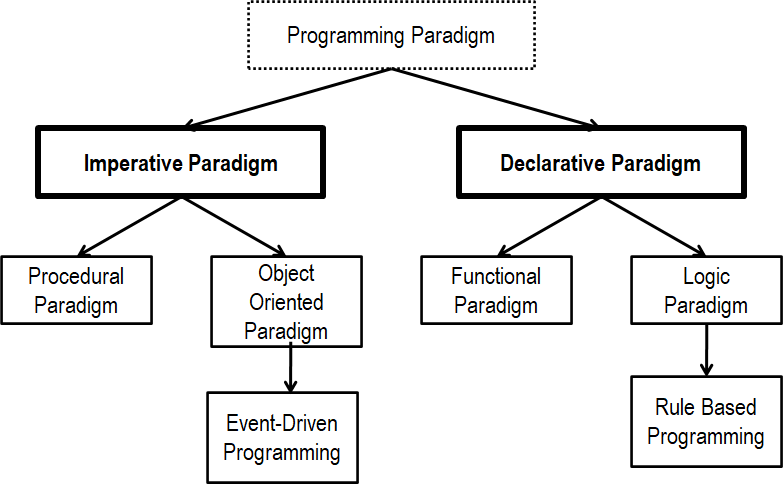
\includegraphics[width=0.75\textwidth]{../figures/paradimas_simao.png}
  \caption{Classificação dos paradigmas de programação com os paradigmas emergentes}
  \caption*{Fonte: Autoria própria}
  \label{fig:paradigmas_simao}
\end{figure}

\subsection{Paradigmas Imperativos}\label{sec:imperativos}

Nesta seção busca-se apresentar os paradigmas imperativos, ou subparadigmas
imperativos conforme o ponto de vista, mencionados na Seção
\ref{sec:paradigmas}, de modo a estabelecer a sua relação e características em
comum, assim como suas peculiaridades. Os subparadigmas que seguem os princípios
do Paradigma Imperativo (PI) se caracterizam pela flexibilidade de programação e
pela forma explicitamente sequencial pela qual as instruções são executadas
\cite{msc_Banaszewski_2009}. O Paradigma Procedimental (PP) foi o primeiro,
propriamente dito, paradigma de programação proposto, o qual faz parte do âmago
do PI. Posteriormente surge uma forma mais avançada de desenvolvimento em PI,
conhecida como Paradigma Orientado a Objetos (POO) \cite{msc_Banaszewski_2009}.
O PP e o POO se diferenciam pela forma como os elementos e instruções são
organizados, sendo o POO considerado mais rico e estruturado em termos de
abstração e expressão do código \cite{doc_ronszcka_2019}.

\subsubsection{Paradigma Procedimental (PP)}

O Paradigma Procedimental (PP) define um estilo de programação baseado na
organização sequencial de variáveis e comandos, na qual as variáveis representam
os estados das entidades e os comandos executam ações sobre estes estados
\cite{watt_2004,brookshear_2006}. O PP ainda vigora pelos motivos de
considerável coeficiente de modularização, certa simplicidade de programação em
sistemas de menor escala e relativa eficiência, uma vez que a forma de
codificação dos comandos condiz com a forma pela qual os mesmos são executados
pela máquina. Este fato facilita a geração de executáveis enxutos e eficientes
\cite{msc_Banaszewski_2009}. Outro fator que contribui para a permanência deste
paradigma é a experiência adquirida há anos pelos programadores neste tipo de
linguagem, o que é aqui chamado de inércia cognitiva. Neste sentido, alguns
exemplos clássicos de linguagens baseadas no PP são FORTRAN, COBOL, ALGOL,
BASIC, PASCAL e C \cite{msc_Banaszewski_2009}.

Como exemplo de programa no PP, o Código \ref{cod:alarm_c} apresenta um programa
que executa a lógica de tomada decisão sobre o estado de um dado uma aplicação
de sensor, cujo funcionamento já foi descrito na Seção \ref{sec:pon} sob a forma
de \textit{Rules}. Esse exemplo é também utilizado nas seções seguintes de forma a
ilustrar o uso dos diversos paradigmas. Esta implementação no PP é feita de
forma simples, na clássica linguagem de programação C, implementando o
\textit{Sensor} como uma \textit{struct} (estrutura) com duas variáveis membros, sendo
declaradas funções auxiliares para alterar os valores destas variáveis da
\textit{struct} utilizando ponteiros. Adicionalmente, a verificação dos estados
do \textit{Sensor} é feita por meio de um laço de repetição na função
\textit{main}.

\lstinputlisting[language=C++, float=htb, caption = {Exemplo de aplicação de
      sensor em C}, source = {Autoria própria}, label = {cod:alarm_c}]
{../code/ex_pp.cpp}

Em que pese suas vantagens, o PP apresenta certas deficiências, de tal forma que
subsequentemente e mais recentemente, o PP perdeu espaço considerável para o
POO. O PP é limitado no que diz respeito à sua capacidade de representar
abstrações, não possuindo ferramental que realmente induza à coesão de variáveis e
procedimentos diretamente relacionados, por exemplo. O PP só possui um único
mecanismo explícito de modularização, para favorecer a coesão, que é a divisão
do programa em rotinas. Neste sentido, novas ferramentas que aumentam a
capacidade de abstração do PP são introduzidas com o Paradigma Orientado a
Objetos (POO) \cite{Avacheva_2020}.

\subsubsection{Paradigma Orientado a Objetos (POO)}

O Paradigma Orientado a Objetos (POO) apresenta um nível de abstração mais alto
que o PP. Os programas desenvolvidos em POO são compostos por entidades
modulares denominadas objetos, que podem ser entendidas como abstrações de uma
entidade real ou imaginária, contendo as características pertinentes para sua implementação
computacional \cite{poo_2007}. Esses objetos agrupam atributos (similar às
variáveis do PP) e métodos (similar às funções do PP), organizados de maneira a
estimular coesão e desacoplamento, tudo à luz de seus tipos ou classes que ditam
o modelo de suas instâncias, incluindo os seus relacionamentos para com outros
objetos \cite{watt_2004,brookshear_2006,pressman_2016,msc_santos_2017}. Exemplos
de linguagens que materializam este paradigma são a SIMULA, Smalltalk, C++, JAVA
e C\# \cite{msc_Banaszewski_2009}.

Como exemplo do POO, no Código \ref{cod:alarm_cpp} é apresento um programa em
C++ que executa a lógica de tomada decisão sobre o estado de um dado uma
aplicação de sensor, cujo funcionamento é descrito na Seção \ref{sec:pon} sob a
forma de \textit{Rules}. Esse exemplo foi também apresentado anteriormente como
exemplo de implementação para o PP. A diferença entre a aplicação do POO e do PP
é justamente o encapsulamento da entidade \textit{Sensor}, agora implementada
por meio de uma classe com métodos próprios.

\lstinputlisting[language=C++, caption = {Exemplo de aplicação de sensor em
      C++}, source = {Autoria própria}, label = {cod:alarm_cpp}, float=htb]
{../code/ex_poo.cpp}

\subsubsection{Considerações Sobre os Paradigmas Imperativos}

Programas desenvolvidos com POO ou com o PP são concebidos como sequências de
instruções. Esse mecanismo de execução sequencial consiste em buscas, por assim
dizer, ou, mais precisamente, percorrimentos sobre entidades passivas (as
variáveis, os atributos e afins, vetores destes, estruturas de dados desses e
afins) que correspondem aos dados. Isto se dá por meio de comandos de decisão
(\textit{e.g.}, \textit{if-else} e \textit{switch} em linguagem C/C++), sendo
estes executados em laços de repetição (\textit{e.g.}, \textit{for},
\textit{while}, \textit{do-while} em linguagem C/C++) \cite{msc_santos_2017}.

Devido à sequencialidade da busca/percorrimentos e à passividade dos elementos
presente nas linguagens do PP e do POO, trechos de código tendem a se tornar
interdependentes, levando a acoplamentos, bem como há ainda correlatos problemas
de redundância na execução dos programas. Neste âmbito, as expressões causais
são avaliadas passivamente ocasionando as chamadas redundâncias temporais e
estruturais \cite{msc_Banaszewski_2009}. A redundância temporal, ocorre quando
há a reavaliação de expressões causais desnecessárias na presença de estados já
avaliados e inalterados, enquanto redundância estrutural ocorre quando o
conhecimento sobre um estado resultante da avaliação de uma expressão lógica não
é compartilhado entre outras expressões causais pertinentes em diferentes partes
do código, causando reavaliações desnecessárias. No pseudocódigo do Código
\ref{cod:loops} a redundância temporal é observada na linha 2, pelo laço de
repetição \textit{while(true)}, enquanto a redundância estrutural é
exemplificada nas linhas 3 e 12, nas quais o mesmo atributo \textit{attribue\_1}
do \textit{object\_1} é avaliado redundantemente nos dois \textit{ifs}. Estes
problemas podem afetar o desempenho dos programas desenvolvidos
\cite{msc_Banaszewski_2009}.

\begin{lstlisting}[numbers=left,
  stepnumber=1, caption = {Exemplo de
  redundâncias estruturais e temporais}, float=htb, source = {Autoria própria}, label =
  {cod:loops}]
...
while (true) do
    if ((object_1.attribute_1 == 1) and
        (object_1.attribute_2 == 1) and
        (object_1.attribute_3 == 1))
    then
        objetct_1.method_1();
        objetct_2.method_1();
        objetct_2.method_1();
    ...
    end_if
    if ((object_1.attribute_1 == 1) and
        (object_1.attribute_n == n) and
        (object_1.attribute_n == n))
    then
        objetct_1.method_n();
        objetct_2.method_n();
        objetct_2.method_n();
    ...
    end_if
end_while
...
\end{lstlisting}

\subsection{Paradigmas Declarativos}\label{sec:declarativos}

Da mesma forma como foi mostrado na Seção \ref{sec:imperativos} em relação aos
Paradigmas Imperativos, esta seção apresenta os Paradigmas Declarativos, de modo
a estabelecer a sua relação e características em comum assim como suas
peculiaridades. Os subparadigmas que seguem o PD, por sua vez seriam o Paradigma
Funcional (PF) e particularmente o Paradigma Lógico (PL), sabendo que, na verdade,
o PF estaria em uma fronteira com PI. 

Em todo caso, os subparadigmas PF e PL do PD caracterizam-se e diferenciam-se
dos subparadigmas do PI puro ao apresentar modelo menos flexível, porém mais
simplificado de programação. Mesmo no PF e certamente no PL, o programador se
concentraria mais na organização do conhecimento  em alto nível sobre a
resolução do problema computacional em si ao invés da implementação mais técnica
propriamente dita \cite{doc_ronszcka_2019}.

Enquanto o PI em geral impõe pesquisas orientadas a laços de repetições sobre
elementos passivos, relacionando dados a expressões causais, o PD possui
soluções declarativas que trabalham por recursões e/ou mecanismos de inferência.
Inclusive, alguns destes mecanismos no PL permitem evitar parte das redundâncias de
execução, conforme discutido no decorrer desta seção \cite{doc_ronszcka_2019}. 

%Dentre
%elas podem ser citados os Sistemas Baseados em Regras (SBRs), que tem como base
%algoritmos de inferência otimizados como o RETE \cite{forgy_1982}, o TREAT
%\cite{miranker_1987}, o LEAPS \cite{miranker_1990} e o HAL \cite{lee_2002}. Sem
%a aplicação destas soluções eficientes ciclos de inferência se tornariam muito
%lentos, inviabilizando a sua utilização em muitos casos \cite{doc_simao_2005}.

\subsubsection{Paradigma Funcional (PF)}

O Paradigma Funcional (PF) é baseado no conceito de funções computáveis por meio
do cálculo \textit{lambda}, que é um conceito que foi matematicamente
introduzido em 1936 por Alonzo Church \cite{henk_1984}. A essência do PF é a
construção de programas a partir da manipulação de dados por meio de funções, em
um modelo no qual as funções podem invocar outras funções ou até mesmo serem
passadas como parâmetros para outras funções
\cite{scott_2000,msc_Banaszewski_2009}. As funções do PF são ditas puras, no
sentido que seu resultado depende apenas da sua entrada, devido às funções não
possuírem estado compartilhado interno \cite{scott_2000}.

No Código \ref{cod:sensor_clj} o mesmo exemplo da aplicação de sensores é
apresentado, desta vez implementado no Paradigma Funcional por meio do uso da
linguagem Clojure, que é um dialeto dinâmico e funcional da linguagem de
programação Lisp.

Uma das vantagens desse paradigma é permitir a programação em mais alto nível
que o PP e POO puras justamente por permitir flexibilidades como a passagem de
funções como parâmetros. Além disso, o uso de funções puras facilita o
paralelismo, pois não existe estado compartilhado
\cite{scott_2000,bhadwal_2020}. Em contrapartida, a falta de estado
compartilhado combinado com recursão pode e tende a causar redução no desempenho
do programa \cite{bhadwal_2020}. Adicionalmente, ainda que o estilo de
programação funcional supostamente facilite escrever as funções, ele dificulta a
integração com outras áreas do código, principalmente operações de entrada e
saída de dados, como no caso interfaces e arquivos \cite{bhadwal_2020}.

\begin{lstlisting}[caption = {Exemplo de
aplicação de sensor em Clojure}, float=htb, source = {Autoria própria}, label =
{cod:sensor_clj}]
;; Autoria: Gustavo Brunholi Chierici - Data 22/06/2021 - Grupo de Pesquisa: PON - UTFPR

(defrecord FPSensor [is-read is-activated])     ;; Record ("struct") do sensor

(defn create-sensor [] (FPSensor. false false)) ;; Função que retorna um sensor

(defn activate-sensor                           ;; Função que "ativa" o sensor
    [sensor]
    (assoc sensor :is-activated true :is-read false))

(defn deactivate-sensor                         ;; Função que "desativa" o sensor
    [sensor]
    (assoc sensor :is-activated false))

(defn read-sensor                               ;; Função que "lê" o sensor
    [sensor]
    (assoc sensor :is-read true))

(defn check-sensor                              ;; Função que verifica se o sensor está ativado e o "lê" em caso positivo
    [sensor]
    (if (and (:is-activated sensor) (not (:is-read sensor)))
        (deactivate-sensor (read-sensor sensor)) sensor))
\end{lstlisting}

Alguns exemplos de linguagens baseadas no PF são LISP, Clojure, Miranda,
Haskell, Sisal, pH e ML \cite{msc_Banaszewski_2009}. Além destas linguagens,
C++11 em diante, C\# 3.0 e Java 8 também adicionaram construções que facilitam o
desenvolvimento de programas no estilo funcional, ainda que de forma híbrida e
dominada por seus paradigmas de origem \cite{bhadwal_2020}.

\subsubsection{Paradigma Lógico (PL)}

Apesar dos subparadigmas apresentados anteriormente (PP, POO e mesmo PF) se
basearem em teorias diferentes, eles acabam compartilhando a mesma forma de
execução em alguma medida. Mais precisamente, em todos eles, um programa ou
mesmo uma função, recebe dados como entrada, realiza computações e gera uma
saída via um mapeamento direto interno. Este processo é definido como um
mapeamento da entrada para a saída do programa
\cite{watt_2004,msc_Banaszewski_2009}.

No PL, além das entidades com suas variáveis e comandos usuais (\textit{i.e.},
base de fatos) em formas como frames (aparentados de objetos, mas com métodos
suspostamente simples ou pragmáticos), os comandos lógicos causais também são
representados na forma de dados, sob o viés de regras (\textit{i.e.}, base de
regras) conforme Figura \ref{fig:rule_pl}. Não raro, linguagens e ambientes do
PL são chamados Sistemas Baseados em Regras (SBRs) justamente. Em todo caso,
essa relação entre base de fatos e base de regras, buscando aprovar/desaprovas
regras pelas suas confrontações, dá-se pela busca realizada por meio de algum
mecanismo de inferência sobre as definições de elementos factuais (e.g., frames)
da base de fatos vis-à-vis expressões causais (normalmente regras) da base de
regras, conforme Figura \ref{fig:fact_base} \cite{msc_Banaszewski_2009}. Isto
dito, alguns exemplos de linguagens que implementam o PL são  Oz
\cite{van_roy_2004}, Prolog, RuleWorks e OPS \cite{msc_Banaszewski_2009}.

\begin{figure}[!htb]
\centering
\subcaptionbox{Entidades}{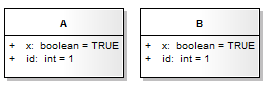
\includegraphics[width=0.50\textwidth]{../figures/ab_pl.png}}%
\hfill
\subcaptionbox{Regra}{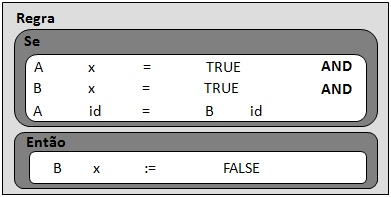
\includegraphics[width=0.50\textwidth]{../figures/rule_pl.png}}%
\caption{Conhecimento representado em regras no PL}
\caption*{Fonte: \citeonline{msc_Banaszewski_2009}}
\label{fig:rule_pl}
\end{figure}

Ainda, há linguagens do PL, como OPS e Ilog Rules, que tem como base algoritmos
de inferência otimizados como o RETE \cite{forgy_1982}. Outros exemplos de
algoritmos de inferência otimizados são TREAT \cite{miranker_1987} e o LEAPS
\cite{miranker_1990} derivados do RETE, bem como o alternativo o HAL
\cite{lee_2002}. Sem a aplicação destas soluções eficientes ciclos de inferência
se tornariam muito lentos, inviabilizando a sua utilização em muitos casos.
Entretanto, mesmo com algoritmos de inferência considerados eficientes, ainda há
redundância de processamentos e preço de representar base de fatos e base de
regras em estrutura de dados \cite{doc_simao_2005,msc_Banaszewski_2009}.

\begin{figure}[!htb]
  \centering
  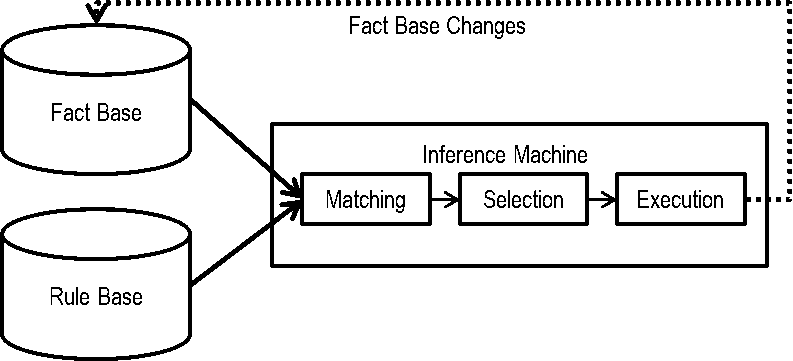
\includegraphics[width=0.6\textwidth]{../figures/fact_base.png}\smallskip
  \caption{Arquitetura interna de um Sistema Baseado em Regras}
  \caption*{Fonte: \citeonline{msc_Banaszewski_2009}}
  \label{fig:fact_base}
\end{figure}

O RETE em particular implementa um processo de busca otimizado, manipulando
elementos da base de fatos e regras sobre uma estrutura baseada em redes ou
grafos. Esse processo é ilustrado de forma simplificada na Figura
\ref{fig:rete}. Mais precisamente, o RETE guarda informação sobre avaliações
anteriores das regras e também avalia as regras somente quando a base de fatos é
atualizada de modo a evitar avaliações redundantes, ou seja, quando um elemento
da base de fatos é inserido/modificado/removido da Base de Fatos. Com isto, o
RETE resolve o problema das redundâncias temporais do PI. Esta solução se faz
possível porque o RETE é composto de duas sub-redes: a $\alpha$-network é composta
por nós sendo cada qual responsável pela avaliação lógica de fatos; a
$\beta$-network, por sua vez, é composta por outros nós, sendo cada qual
responsável pela correlação entre fatos. Se as avaliações e correlações forem
satisfeitas para uma regra, a mesma é aprovada sendo, portanto, inserida no
conjunto de conflito
\cite{forgy_1982,doorenbos_1995,msc_Banaszewski_2009}

\begin{figure}[!htb]
  \centering
  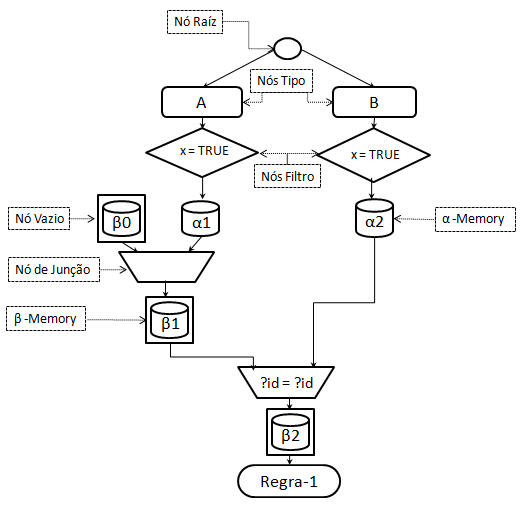
\includegraphics[width=0.65\textwidth]{../figures/inference_machine.png}
  \caption{Estrutura do algoritmo RETE}
  \caption*{Fonte: \citeonline{msc_Banaszewski_2009}}
  \label{fig:rete}
\end{figure}

No Código \ref{cod:sensor_ruleworks} novamente o exemplo da aplicação de tomada de
decisão sobre um sensor é apresentado, desta vez implementado no Paradigma
Lógico com a linguagem de programação RuleWorks. Observa-se que, por se tratar
de uma linguagem de programação cuja estrutura se baseia em regras, o código tem
apresenta muita similaridade ao representado sob a forma de \textit{Rule} na
Figura \ref{fig:nop_rule}.

\begin{lstlisting}[
  caption = {Exemplo de aplicação de sensor em RuleWorks},
  float=htb,
  source = {Autoria própria},
  label = {cod:sensor_ruleworks}
]
(object-class sensor
    ^is-read
    ^is-activated
)

(rule process-sensor:sensor
    (sensor ^$ID <the-sensor> ^is-read <false> ^is_activated <true>)
    -->
    (bind <the-sensor ^is-read> (false))
    (bind <the-sensor ^is-activated>  (false))
)
\end{lstlisting}

\subsubsection{Considerações Sobre os Paradigmas Declarativos}

O PD se propõe a resolver algumas das deficiências do PI, principalmente aquelas
relacionadas à dificuldade de programação em ambientes \textit{multicore},
atualmente no caso do PL contemporâneo, e redundâncias estruturais e temporais,
no caso do PL/SBR com máquinas de inferência apropriadas. Apesar disso, a
maioria destas deficiências ainda se repete devido aos mecanismos de execução
tanto do PF como do PL que se baseiam em buscas sob elementos passivos, que por
sua vez ou reproduzem estes mesmos problemas de redundâncias estruturais e
temporais e/ou os atenuam com algoritmos inferência dito otimizados, mas trocando
os problemas por estruturas de dados caras. Assim, normalmente programas em PD
são mais lentos que em PI, apesar das redundâncias deste
\cite{msc_Banaszewski_2009}.

Além disso, enquanto as linguagens de programação do PD apresentam um modelo de
programação mais simplificado, elas também não oferecem a mesma flexibilidade
das linguagens do PI. Isto pode dificultar a construção de códigos mais
eficientes, visto que limita o controle que o programador tem sobre o
\textit{software}. Finalmente, mesmo no caso de PF, tanto em PD quanto PI em
geral, a orientação a buscas e/ou percorrimentos deles não permite alcançar
facilmente módulos desacoplados, particularmente em nível granular, o que
dificulta processamentos paralelo e/ou distribuídos \cite{msc_Banaszewski_2009}.

\subsection{Paradigmas Emergentes}

Em suma, como já dito, os paradigmas dominantes PI (com PP e POO) e PD (com PF e
PL) tendem a ter problemas similares de redundâncias e/ou processamentos e
acoplamentos. Isto dificulta alcançar demandas contemporâneas como a facilitação
de programação em alto nível, boa performance de processamento e boa performance
do paralelismo/distribuição de processamento em arquiteturas com múltiplos
núcleos, por exemplo. 

Outrossim, além dos paradigmas dominantes, há os paradigmas emergentes que não
raro se materializam sobre os dominantes. Muito embora emergentes conhecidos não
tenham resolvidos esses problemas relatados dos dominantes, eles sim trazem
novas conotações de desenvolvimento. Exemplos de paradigmas emergentes (talvez
mais conhecidos) são como Paradigma Orientado a Componentes (POC), Paradigma
Orientado a Eventos (POE), Paradigma Orientado a Aspectos (POA), Paradigma
Orientado a Agentes (POAg) e Paradigma Orientado a Atores (POAt).


\subsubsection{Paradigma Orientado a Componentes (POC)}

O Paradigma Orientado a Componentes (POC) se baseia no reuso e combinação de
componentes. Um componente consiste em uma parte do programa desenvolvida de
forma a ser altamente reutilizável, que pode ser desenvolvida independentemente
para ser depois combinada com outras partes objetivando construir uma unidade
maior \cite{dsouza_1998}.

Na Figura \ref{fig:componentes} um diagrama de componentes é exemplificado, no
qual os componentes se relacionam para realizar o fluxo de execução do programa.
As setas direcionais representam a invocação de serviços oferecidos por estes
componentes. Os serviços não são acessados diretamente, mas por meio de
entidades descritoras, chamadas de interfaces. O uso de interfaces é uma
característica do POC que permite que a definição dos serviços seja feita
completamente separada da implementação \cite{crnkovic_2002}

\begin{figure}[!htb]
  \centering
  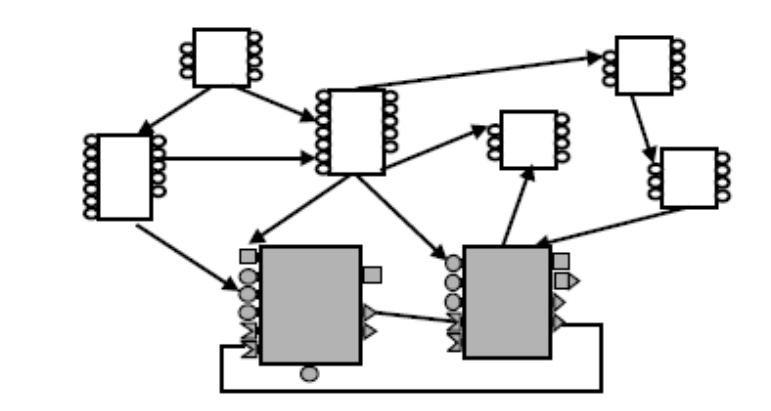
\includegraphics[width=0.8\textwidth]{../figures/componentes.png}
  \caption{Diagrama de componentes}
  \caption*{Fonte: \citeonline{crnkovic_2002}}
  \label{fig:componentes}
\end{figure}

O POC é muito utilizado em \textit{frameworks} de programação de
\textit{front-end}, como React\footnote{Para maiores detalhes sobre este
\textit{framework}, consultar \url{https://reactjs.org/}}, Angular\footnote{Para
maiores detalhes sobre este \textit{framework}, consultar
\url{https://angular.io/}} e VUE\footnote{Para maiores detalhes sobre este
\textit{framework}, consultar \url{https://vuejs.org/}}. No Código
\ref{cod:components_js}, é mostrado o exemplo de tomada de decisão sobre um
sensor em linguagem de programação JavaScript com o \textit{framework} Angular,
na qual pode ser observado que a implementação do sensor importa e implementa a
funcionalidade do componente \textit{OnInit}.

\begin{lstlisting}[caption = {Exemplo de aplicação de sensor em React no POC},
source = {Autoria própria}, float=htb,
label  = {cod:components_js}]
/* Autoria: Prof. Dr. Roni Fabio Banaszewski - Data 24/06/2021 - Grupo de Pesquisa: PON - UTFPR */ 

import {Component, OnInit} from '@angular/core';
import {BehaviorSubject} from "rxjs";

@Component({
  selector: 'app-root',
  templateUrl: './app.component.html',
  styleUrls: ['./app.component.css']
})

export class AppComponent implements OnInit {
  title = 'sensor-app';

  ready: boolean = false;
  active: boolean = true;

  private readySubject = new BehaviorSubject<boolean>(this.ready);
  private activeSubject = new BehaviorSubject<boolean>(this.active);

  ngOnInit() {
    this.readySubject.subscribe(value => {
      this.ready = value;
      this.rule()
    });

    this.activeSubject.subscribe(value => {
      this.active = value;
      this.rule()
    });
  }

  rule() {
    if (this.ready == false && this.active == true) {
      this.readySubject.next(true);
      this.activeSubject.next(false);
    }
  }
}
\end{lstlisting}

A principal desvantagem do POC é que o foco na reusabilidade dos componentes
tende a aumentar a complexidade deles, de modo que se torna necessário a
execução de processos mais cuidadosos de planejamento do sistema e manutenção
dos componentes. Quanto mais reutilizável for o componente, mais complexo ele se
torna e mais difícil é a sua manutenção \cite{crnkovic_2002}. Por fim,
internamente o POC é, na prática, o encapsulamento de módulos criados via
paradigmas já existentes.

\subsubsection{Paradigma Orientado a Eventos (POE)}\label{sec:poe}

No Paradigma Orientado a Eventos (POE) as entidades interagem por meio da
ocorrência de eventos. Um evento consiste em uma condição detectável que pode
instigar a execução de um método. O objeto capaz de detectar a condição e gerar
o evento é chamado de objeto transmissor, enquanto os objetos interessados que
recebem um evento são chamados de objetos receptores \cite{ferg_2006}.

A Figura \ref{fig:eventos} ilustra a relação entre os objetos transmissores e
receptores, que podem ocorrer de forma direta ou indireta. No exemplo à esquerda
na Figura \ref{fig:eventos}, um objeto transmissor detecta a ocorrência de um
evento e notifica este evento diretamente aos objetos receptores interessados.
No exemplo à direita na Figura \ref{fig:eventos}, o evento é transmitido por
intermédio do objeto \textit{Dispatcher} \cite{msc_xavier_2014}. A transmissão
do evento ocorre por meio da passagem de um \textit{token}, o qual pode ser
representado por uma mensagem formada por uma cadeia de caracteres ou um objeto
com dados \cite{ferg_2006}.

\begin{figure}[!htb]
  \centering
  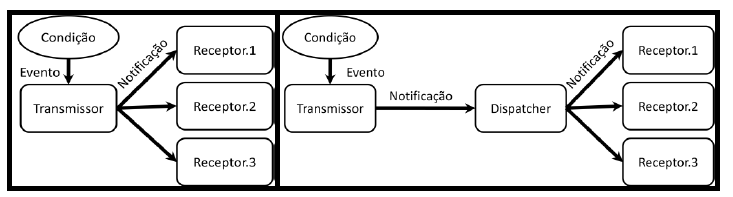
\includegraphics[width=\textwidth]{../figures/eventos.png}
  \caption{Processo de detecção de eventos}
  \caption*{Fonte: \citeonline{faison_2006}}
  \label{fig:eventos}
\end{figure}
\FloatBarrier

Na verdade, não existe linguagem de programação que implementa especificamente o
POE, sendo ele incorporado por \textit{frameworks} e afins nas linguagens dos
paradigmas vigentes. Por exemplo, um \textit{framework} muito popular para C++ e
Python que implementa a orientação a eventos é o Qt\footnote{Para maiores
  detalhes sobre este \textit{framework}, consultar \url{https://www.qt.io/}}. Em
suma, o Qt é um \textit{framework} para a criação de aplicações gráficas de
forma intuitiva, usando técnica para tal conhecida como \textit{Rapid
  Application Development} (RAD). Neste \textit{framework}, um caso muito comum
para o uso de eventos é mostrado no Código \ref{cod:qt_event}, no qual os
eventos são enviados para ativar o sensor ao pressionar um botão, ao conectar o
evento \textit{button.clicked} às funções \textit{Activate()} e
\textit{Process()}.

\begin{lstlisting}[language = Python, float=htb,
  caption = {Exemplo de aplicação de sensor com PyQt5 no POE},
  source = {Autoria própria},
  label = {cod:qt_event}]
class Sensor(QWidget):
    isRead = False
    isActivated = False
    button = QPushButton('Activate')
    
    def Activate(self):
        self.isActivated = True
        self.isRead = False    
    def Deactivate(self):
        self.isActivated = False
        self.isRead = False          
    def Process(self):
        if(self.isActivated and not self.isRead):
            alert = QMessageBox(self)
            alert.setText('Sensor Processed')
            alert.show()
            self.Deactivate()    
    def __init__(self):
        super().__init__()
        self.button.clicked.connect(self.Activate)
        self.button.clicked.connect(self.Process)
        self.button.show()
\end{lstlisting}

Dentre os Paradigmas Emergentes mencionados na Seção \ref{sec:intro_emergentes},
o POE se destaca pelo seu estado de maturidade e extenso uso em diversas
aplicações, desta forma podendo ser considerado um paradigma em fase de
transição de Paradigma Emergente para Paradigma Dominante. Dentre as vantagens
do POE estão a flexibilidade e simplicidade de programação devido ao mecanismo
de eventos, que facilita a interação entre entidades no código, como o botão
\textit{Activate} com o sensor do exemplo. Em contrapartida, o código pode ser
considerado confuso, devido ao fluxo de execução do programa, o que também
dificulta encontrar erros no programa quando comparado a paradigmas com fluxo de
execução mais simples como o do PI ou com lógica em bases de conhecimento
unívocas como em SBR/PL do PD. 

\subsubsection{Paradigma Orientado a Aspectos (POAs)}

O Paradigma Orientado a Aspectos (POAs) permite separar as funcionalidades
principais de funcionalidades secundárias de um código típico orientado a
objetos, encapsulando as funcionalidades secundárias em uma unidade modular
chamada de aspecto. No contexto do POA, a funcionalidade principal é uma
funcionalidade única implementada por determinada função ou método, enquanto as
funcionalidades secundárias são genéricas e compartilhadas entre várias funções
ou métodos \cite{laddad_2003}.

O POAs propõe essa separação por meio do encapsulamento das funcionalidades
secundárias, sob a forma de aspectos, para serem invocadas implicitamente (sem a
declaração da chamada dos métodos explicitamente no código) pelas
funcionalidades principais. Os aspectos são invocados pela chamada dos métodos
que implementam as funcionalidades principais \cite{miles_2004}. A vantagem da
aplicação desse mecanismo seria maior incentivo ao reuso de código e maior
facilidade de entendimento ou alteração do código
\cite{miles_2004}.

Um exemplo de linguagem de programação na qual pode ser realizada a aplicação do
POA é Python, que conta com suporte nativo da linguagem ao POA por meio dos
chamados \textit{decorators}. No exemplo do Código \ref{cod:python_aspect}, no
qual é implementado o exemplo da aplicação de sensor, essa ferramenta é
utilizada para encapsular a verificação dos estados dos atributos do sensor por
meio do aspecto \textit{checker\_aspect}.

\begin{lstlisting}[
language = Python, %float=htb,
  caption = {Exemplo de aplicação de sensor em Python no POAs},
source = {Autoria própria}, float=htb,
label = {cod:python_aspect}]
# Autoria: Marcos Talau e Felipe Neves - Data 26/06/2021 - Grupo de Pesquisa: PON - UTFPR 
def checker_aspect(func):
    def wrapper(self):
        func(self)
        if(self.isActivated and not self.isRead):
            self.Process()
    return wrapper

class Sensor:
    isRead = False
    isActivated = False

    @checker_aspect
    def Activate(self):
        self.isActivated = True
        self.isRead = False
    @checker_aspect
    def Deactivate(self):
        self.isActivated = False
        self.isRead = False
    def Process(self):
        self.Deactivate()
\end{lstlisting}

%TODO: desvantagens POAs

\subsubsection{Paradigma Orientado a Agentes (POAg) / Atores (POAt)}

O Paradigma Orientado a Agentes (POAg) permite construir programas empregando
entidades chamadas agentes. Os agentes são entidades computacionais capazes de
executar ações de maneira flexível e autônoma, de modo a atingir objetivos
estabelecidos no momento da sua concepção \cite{jennings_1999}.

Os agentes são usualmente implementados sobre os conceitos do POO, porém agentes
possuem propriedades mais complexas do que um objeto. Diferente dos objetos, que
atuam passivamente até que um de seus métodos sejam invocados, agentes podem
atuar de forma proativa, tendo objetivos individuais ou coletivos. Um objeto
aguarda até que seja lhe indicado o que fazer, enquanto o agente decide por si
só quando e o que deve ser feito. Ainda, em POAg as relações entre os entes
acontecem na dinâmica do sistema, de maneira fluida e não tudo pré-definido como
normalmente ocorre em POO \cite{msc_Banaszewski_2009}.

No Código \ref{cod:agent_ex}, é mostrado o exemplo de tomada de decisão sobre um
sensorem linguagem de programação Elixir/Erlang. Neste exemplo simples, pode ser
observada a complexidade presente devido às funcionalidades básicas necessárias
para a comunicação entre agentes.

\begin{lstlisting}[caption = {Exemplo de aplicação de sensor em Elixir no POAg}, %float=htb,
source = {Autoria própria}, language=elixir, float=htb,
  label = {cod:agent_ex}]
# Autoria: Fabio Negrini - Data 11/08/2021 - Grupo de Pesquisa: PON - UTFPR
defmodule Sensor do use GenServer
  def create() do
    state = init_state()
    {:ok, pid} = GenServer.start_link(__MODULE__, state, name: __MODULE__)
    pid
  end
  defp init_state() do
    %{:is_read   => false,
      :is_activated => false}
  end
  @impl true
  def init(stack) do
    {:ok, stack}
  end
  @impl true
  def handle_call(:is_read, _from, state) do
    is_read = Map.get(state, :is_read)
    {:reply, is_read, state}
  end
  def handle_call(:is_activated, _from, state) do
    is_activated = Map.get(state, :is_activated)
    {:reply, is_activated, state}
  end
  @impl true
  def handle_cast(:activate, state) do
    state = Map.put(state, :is_read, false)
    state = Map.put(state, :is_activated, true)
    {:noreply, state}
  end
  def handle_cast(:read, state) do
    state = Map.put(state, :is_read, true)
    {:noreply, state}
  end
  def handle_cast(:deactivate, state) do
    state = Map.put(state, :is_activated, true)
    {:noreply, state}
  end
end
\end{lstlisting}

O Paradigma Orientado a Atores (POAt) é consideravelmente similar ao POAg, sendo
o modelo de agentes uma extensão do modelo de atores. A diferença entre agentes
e atores é que os agentes são tipicamente mais complexos e capazes de tomada de
decisão lógica \cite{cardoso_2013}. As principais linguagens do POAt são Akka e
Erlang. Ambos os modelos do POAt e POAg trazem a vantagem de facilitar o
paralelismo devido ao alto desacoplamento entre as entidades, enquanto uma das
principais desvantagens é o alto tempo de execução da comunicação entre os
atores/agentes.

\subsection{Considerações Sobre os Paradigmas Dominantes e Emergentes}

Esta seção permitiu contextualizar as principais características, como vantagens
e desvantagens dos paradigmas de programação atuais, tanto dos dominantes como
dos emergentes. Na Seção \ref{sec:motiv} foram levantadas as principais demandas
do desenvolvimento de \textit{software} atuais, que seriam a programação em alto
nível, paralelismo e desempenho. Nesse sentido, nenhum dos Paradigmas Dominantes
atende de forma simultânea a todas essas demandas. Conforme detalhado na Tabela
\ref{tab:demandas2}, o PI apesar de apresentar bom desempenho, não possibilita a
programação em alto nível e dificulta a implementação de paralelismo, enquanto o
PD apresenta tais características, porém o faz em troca de desempenho inferior
quando comparado ao PI.

\begin{table}[!htb]
  \centering
  \caption{Demandas de desenvolvimento de \textit{software} atendidas pelos
    Paradigmas Dominantes}
  \caption*{Fonte: Autoria própria}
  \label{tab:demandas2}
  \smallskip
  \begin{tabularx}{\textwidth}{|l||*{6}{X|}}\hline
    \diagbox{Demanda}{Paradigma} & Imperativo    & Declarativo    \\\hline\hline
    Programação em alto nível             &            & \checkmark \\ \hline
    Paralelismo                           &            & \checkmark \\ \hline
    Desempenho                            & \checkmark &            \\ \hline
  \end{tabularx}
\end{table}

De todo modo os Paradigmas Emergentes mencionados também não por herdarem muitas
das defíciencias dos Paradigmas Dominantes. Isto é dado por muitos desses
paradigmas serem construídos com base nos Paradigmas Dominantes, ou
implementados nas linguagens de programação já existentes dos mesmos.
Feita esta revisão geral nesta seção, a seção seguinte enfim apresenta em
maiores detalhes o Paradigma Orientado Notificações (PON).

\pagebreak

\section{Paradigma Orientado Notificações (PON)}\label{sec:estado_arte_pon}

O Paradigma Orientado a Notificações (PON) é uma solução de desenvolvimento de
software que permite, entre outras características, excelente desempenho
computacional via entidades enxutas que colaboram por notificações precisas. O
inovador PON apresenta propriedades que unem a flexibilidade de programação do
Paradigma Imperativo (PI) e a facilidade de programação do Paradigma Declarativo
(PD) \cite{doc_ronszcka_2019,oshiro_2021}. 

Em suma e mais precisamente, o PON proporciona uma nova visão de desenvolver,
estruturar e executar software por meio de entidades facto-execucionais e
lógico-causais que colaboram por notificações precisas e pontuais [Ronszcka
2019]. Com isto, o PON apresenta três propriedades elementares, que consistem
em: (a) facilidade de programação orientada a regras em alto nível, (b) evitar
redundâncias de código lógico-causal que viabiliza alto desempenho de execução e
(c) desacoplamento implícito de construtos que viabiliza paralelismo e
distribuição \cite{doc_ronszcka_2019,oshiro_2021}.

De modo geral, dito de outra forma, o PON resolve certos problemas existentes
nos outros paradigmas de programação atuais (como PI e PD com seus subparadigmas
dominantes ou emergentes), os quais foram pragmaticamente revisados na Seção
\ref{sec:paradigmas} e detalhadamente revisados na literatura pertinente, como
em \citeonline{van_roy_2004,scott_2009,msc_Banaszewski_2009,msc_xavier_2014} e
\citeonline{doc_ronszcka_2019}. Exemplos de problemas dos paradigmas de
programação vigentes são enfim as redundâncias temporais e estruturais na
análise lógico-causal com o consequente mau uso do tempo de processamento, assim
como o acoplamento excessivo entre entidades computacionais que dificulta o
reaproveitamento e paralelização/distribuição das mesmas
\cite{pat_simao_2008,msc_Banaszewski_2009,doc_linhares_2015,msc_pordeus_2017,doc_Kerschbaumer_2018,doc_ronszcka_2019}.

\subsection{Constituintes do PON}

Muito embora o PON já tenha sido apresentado na introdução desta dissertação,
ele é aqui reapresentado de forma objetiva para facilitar o encadeamento da
leitura, bem como para fins de revisão. Substancialmente, o PON é constituído
por dois conjuntos de entidades computacionais: o facto-execucional e o
lógico-causal \cite{doc_ronszcka_2019,oshiro_2021}. A relação entre eles e as
entidades constituintes do PON, são ilustradas, no contexto de um sistema de
correlação de sensores, pela Figura \ref{fig:oshiro_pon}.

Conforme a Figura \ref{fig:oshiro_pon}, há entidades facto-execucionais
notificantes, os Fact Base Elements (FBE), que representam entidades do mundo e
são compostas de sub-entidades Attributes e sub-entidades Methods, as quais
respectivamente retratam seus estados e seus serviços/comportamento. Há também
entidades lógico-causais notificáveis, as Rules, sendo cada qual composta de uma
sub-entidade Condition e uma sub-entidade Action, que respectivamente se
associam à sub-entidades Premises e à sub-entidades Instigations. Em tempo de
construção das entidades, à luz de suas relações, são estabelecidos conexões
para fins de notificações entre elas \cite{doc_ronszcka_2019,oshiro_2021}. Em
suma, o ciclo de notificações funciona assim: cada Attribute de uma instância de
um FBE que mudar de estado notifica apenas as Premises efetivamente pertinentes,
o que faz com que essas refaçam seus cálculos lógicos. Cada Premise que mudar de
estado lógico notifica apenas as Conditions efetivamente pertinentes, fazendo
com que essas refaçam seus cálculos lógicos pelos estados notificados
contabilizados. Por sua vez, se a Condition for aprovada, ela pode aprovar sua
respectiva Rule. Esta, quando aprovada, ativa então sua Action, que notifica
suas Instigations. Estas enfim instigam precisamente os Methods. Estes últimos
geralmente alteram os estados dos Attributes, reativando o fluxo de notificações
\cite{doc_ronszcka_2019,oshiro_2021}.

\begin{figure}[!htb]
  \centering
  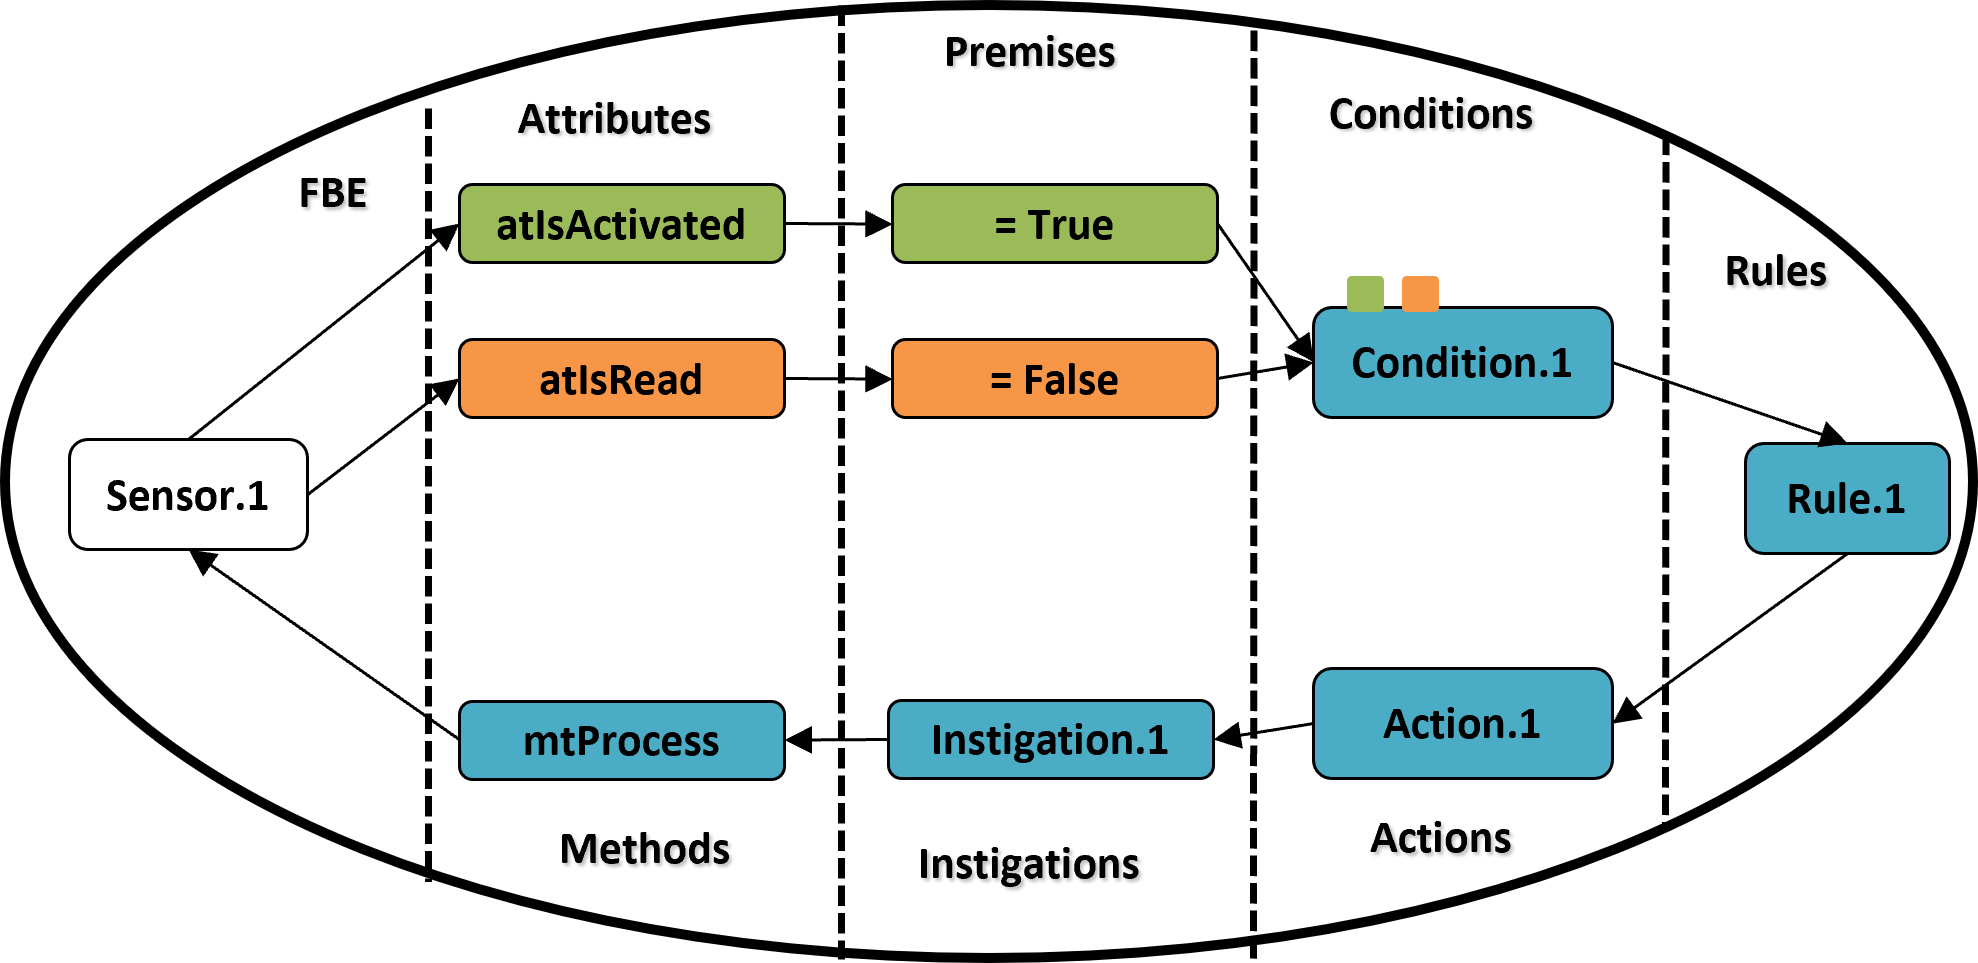
\includegraphics[width=0.9\textwidth]{../figures/nop_cycle.png}
  \smallskip
  \caption{Interação entre as entidades do PON e ciclo de notificações}
  \caption*{Fonte: Autoria Própria}
  \label{fig:oshiro_pon}
\end{figure}

Isto dito, o PON permite o desacoplamento das expressões lógico-causais do resto
do programa, por meio da aplicação destas entidades reativas e notificantes
justamente. Como as entidades apenas trocam notificações, elas não estão
fortemente acopladas entre si, o que é usualmente chamado de desacoplamento.
Essa característica favorece o desenvolvimento de aplicações paralelas e
distribuídas, ao mesmo tempo que mantém o desempenho das aplicações. Isso difere
do modelo de desenvolvimento usual, como no POO do PI e nos SBR do PD, nos quais
as expressões causais são passivas e acopladas a outras partes do programa,
conforme anteriormente elucidado
\cite{pat_simao_2008,simao_2009,msc_Banaszewski_2009,simao_2012a,doc_ronszcka_2019}.

No PON, a entidade reativa que trata a expressão causal é a \textit{Rule},
conforme acima explicado. Assim, cada \textit{Rule} gerencia o conhecimento
sobre o comportamento lógico-causal de um conjunto de \textit{FBEs} que a fazem
reagir pela cadeia de notificação de seus constituintes. Ainda, o conhecimento
lógico-causal de uma \textit{Rule} provém normalmente de uma regra se-então, o
que é uma maneira natural de expressão deste tipo de conhecimento, enquanto o
conhecimento facto-execucional dos FBEs provém em uma forma de expressão
compatível, similar a objetos ou \textit{frames} \cite{doc_ronszcka_2019}.

Uma vez que estas entidades Rules e FBEs são criadas à luz desses conhecimentos
lógico-causais e facto-execucionais, a cadeia de notificações também é
criada/conectada na criação das suas entidades constituintes. Essas entidades
computacionais notificantes precisamente que possibilitam que o mecanismo de
execução ocorra de forma reativa e naturalmente desacoplada, bem como
possibilitam a redução de redundâncias temporais e estruturais, viabilizando
inclusive boa performance e o paralelismo e/ou distribuição fina de
processamento \cite{simao_2012a}. A boa performance, particularmente,
encontraria lastro no cálculo assintótico da complexidade temporal dessas
entidades reativado PON, o que é abordado na seção seguinte.

\subsection{Complexidade temporal}\label{sec:complexidade}

Com base nas entidades reativas e notificantes do PON é possível calcular a
complexidade temporal da execução do mecanismo de notificações.
\citeonline{msc_Banaszewski_2009} define a complexidade assintótica para o pior
caso representada por O(n³) ou O(\textit{FactBaseSize} * \textit{nPremises} *
\textit{nRules}), onde \textit{FactBaseSize} corresponde ao número máximo de
objetos \textit{Attributes}, nPremises corresponde ao número máximo de entidades
\textit{Premises} notificadas por estes \textit{Attributes} e \textit{nRules}
corresponde ao número máximo de entidades \textit{Conditions-Rules} notificadas
por estas \textit{Premises} \cite{doc_simao_2005,msc_Banaszewski_2009}.

Esse cálculo é ilustrado na Figura \ref{fig:calculo_pon}, na qual
\textit{Attributes}, \textit{Premises}, \textit{Conditions} e \textit{Rules}
correspondem respectivamente aos símbolos com abreviações Att, Pr, Cd e Rl.
O caso assintótico considera o pior caso, no qual a alteração do estado do
\textit{Attribute} causa alteração no estado de todas as \textit{Premises}, que
por sua vez notificam todas as \textit{Conditions}, que também notificam todas
as \textit{Rules}. Entretanto, em um caso típico, a alteração do estado de um
\textit{Attribute} nem sempre causa alteração no estado de qualquer
\textit{Premise} ou \textit{Condition}, de forma que não são geradas tantas
notificações, permitindo um melhor desempenho do que o considerado no cálculo
assintótico.

Entretanto, ao invés de se considerar apenas o pior caso, pode ser analisada a
complexidade do caso médio. Neste caso, a análise da complexidade é iniciada no
começo do processo de notificação do PON, a partir da entidade
\textit{Attribute}. Desta forma, as principais variáveis envolvidas na
notificação de um \textit{Attribute} seriam $FBat() = nPremises * nRules$. A
variável \textit{nPremises} é a soma do número de entidades \textit{Premises} a
serem notificadas por dado \textit{Attribute} e a variável \textit{nRules} é a
soma do número de entidades \textit{Rules} dependentes da mudança de estado de
\textit{Premises} consideradas em \textit{nPremises}. Portanto, se for
considerado um ciclo de notificações como a notificação gerada por de um único
\textit{Attribute} e $n$ como sendo o número de total de \textit{Attributes} do
sistema, a complexidade temporal pode ser definida como $(FBat_{1}()+ ... +
FB_{n}()) / n$. Assim, o resultado desta média seria uma constante, o que
implicaria em uma complexidade linear $O(n)$ para o PON
\cite{doc_simao_2005,msc_Ronszcka_2012,doc_ronszcka_2019}.

\begin{figure}[!htb]
  \centering
  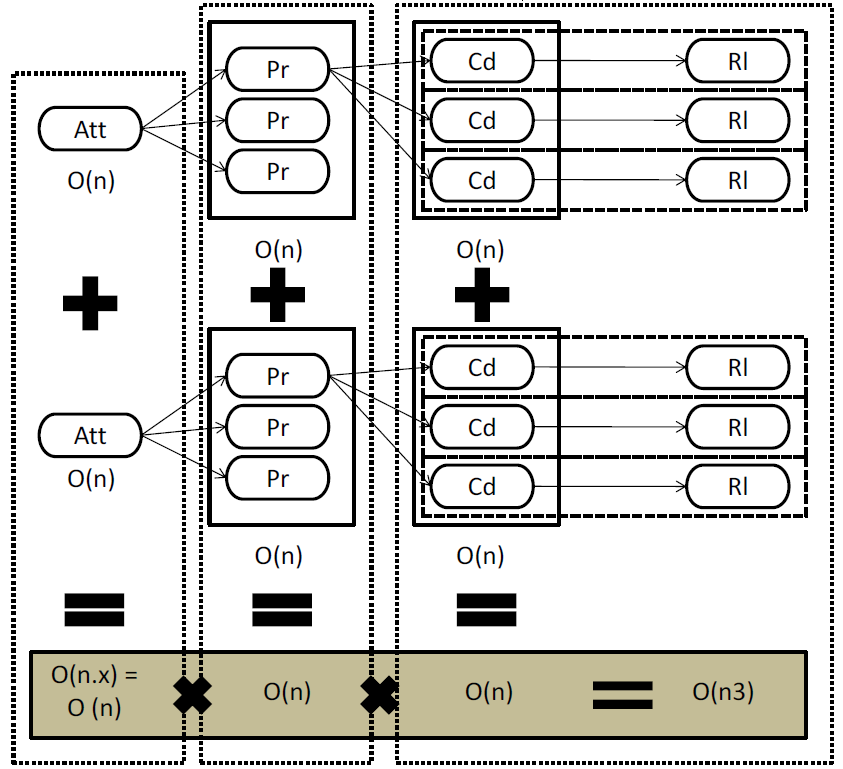
\includegraphics[width=0.8\textwidth]{../figures/calculo_pon.png}
  \smallskip
  \caption{Cálculo assintótico do mecanismo de notificações}
  \caption*{Fonte: \citeonline{msc_Banaszewski_2009}}
  \label{fig:calculo_pon}
\end{figure}

\section{Conceitos de programação ou desenvolvimento em
  PON}\label{sec:conceitos_pon}

Desde as subseções \ref{sec:reatividade} até \ref{sec:agregacao} se apresentam
os diversos conceitos de programação ou desenvolvimento em PON, introduzidos com
o objetivo de facilitar o desenvolvimento de aplicações em PON, sendo que não
necessariamente cada materialização (\textit{i.e.}, implementação) do PON as
contemplam na sua totalidade.

\subsection{Reatividade das entidades}\label{sec:reatividade}

No PON, a reatividade das suas entidades é um conceito central. Neste âmbito, as
entidades reativas do PON conseguem gerar as notificações pontuais entre si, de
acordo com a alteração dos seus estados, que ditam o fluxo de execução do
programa em PON. De maneira geral, a reatividade presente nas entidades
definidas no metamodelo do PON proporciona uma execução livre de avaliações
lógico-causais redundantes e desnecessárias. 

A reatividade das entidades na cadeia de notificações do PON permite evitar a
redundância temporal ao avaliar as expressões lógico-causais somente após a
mudança de estado dos \textit{Attributes} e suas respectivas \textit{Premises}.
Ainda, esta reatividade encontra respaldo no fato de \textit{Conditions} poderem
compartilhar a colaboração de \textit{Premises}, o que evita a redundância
estrutural nas avaliações lógico-causais. Por fim, a reatividade em PON pode ser
melhorada de algumas formas, como por meio de tabelas \textit{hash} nos
Attributes, permitindo que \textit{Premises} recebam notificações de apenas
certos estados de interesse, mas não dos estados que não são de seus interesses
\cite{msc_Banaszewski_2009}. Estes cenários de notificação de \textit{Premises}
tanto com uma lista encadeada simples como com uma tabela \textit{hash} são
ilustrados na Figura \ref{fig:hash_not}, onde um \textit{Attribute}
\textit{atSignal} tem seu estado alterado de vermelho (\textit{RED}) para verde
(\textit{GREEN}), sendo que as setas partindo do \textit{Attribute} representam
as notificações realizadas \cite{msc_Banaszewski_2009}.

\begin{figure}[!htb]
  \centering
  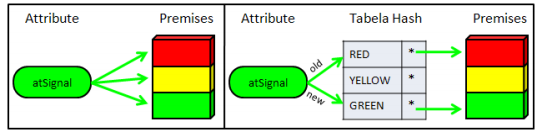
\includegraphics[width=\textwidth]{../figures/hash_not.png}
  \smallskip
  \caption{Notificações baseadas em lista encadeada e tabela \textit{hash}}
  \caption*{Fonte: \citeonline{msc_Banaszewski_2009}}
  \label{fig:hash_not}
\end{figure}

\subsection{Renotificações}

Os \textit{Attributes}, pela sua definição, notificam as \textit{Premises}
apenas quando seu estado é alterado. Porém, em determinados cenários, pode haver
a necessidade de execução de uma \textit{Rule} mesmo quando não há a alteração
no estado dos \textit{Attributes}. Tome-se como exemplo uma \textit{Rule}
responsável (via sua \textit{Action} e dada \textit{Instigation}) pela
instigação da execução de determinado \textit{Method} que precise ser
constantemente reinstigado enquanto a \textit{Condition} daquela \textit{Rule}
estiver verdadeira \cite{msc_Banaszewski_2009}.

Neste tipo de contexto que se faz necessário implementar alguma solução, como o
chamado mecanismo de renotificações. No diagrama de atividades da Figura
\ref{fig:renotif_activity}, é ilustrado o processo de decisão para a geração de
notificação em entidades que suportam o mecanismo de renotificação. Com a
utilização do mecanismo de renotificações, a notificação é gerada mesmo quando
não ocorre uma mudança de estado. À luz da Figura \ref{fig:renotif_activity},
pode-se definir uma frequência para definir (\textit{setar}) estado, permitindo
que a cadeia de notificações seja animada com uma dada cadência
\cite{msc_Banaszewski_2009}.

\begin{figure}[!htb]
  \centering
  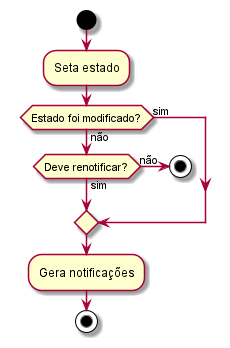
\includegraphics[width=0.4\textwidth]{../out/diagrams/renotification/renotif.png}
  \smallskip
  \caption{Diagrama de atividades do processo de renotificação}
  \caption*{Fonte: Autoria própria}
  \label{fig:renotif_activity}
\end{figure}

\FloatBarrier

Para exemplificar mais precisamente esse cenário de renotificações, tome-se o
exemplo de \textit{Rule} para um alarme apresentado na Figura
\ref{fig:ex_rule_renotif}. Neste caso é considerado que o mecanismo de ativação
da sirene, implementado por meio de \textit{mtRingSirenMilliseconds}, permanece
ativado por um tempo limitado após ser instigado (100 ms neste exemplo). Deste
modo se torna necessário que a cada nova atribuição de valor para
\textit{atStatus} do \textit{FBE} Sensor, seja executada novamente a
\textit{Rule}, o que é feito com a utilização do mecanismo de renotificação.

\begin{figure}[!htb]
  \centering
  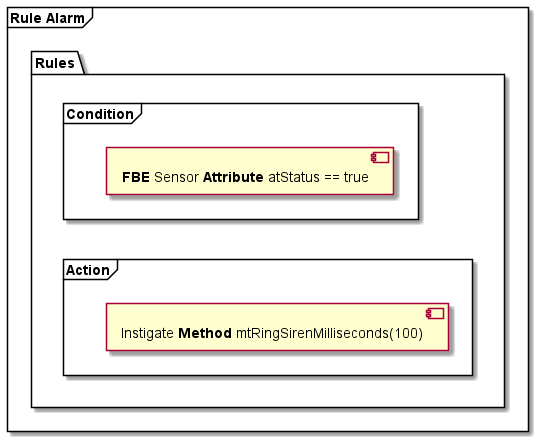
\includegraphics[width=0.6\textwidth]{../out/diagrams/rule_renotif/rules_renotif.png}
  \smallskip
  \caption{\textit{Rule} que depende do mecanismo de renotificações}
  \caption*{Fonte: Autoria própria}
  \label{fig:ex_rule_renotif}
\end{figure}

\subsection{\textit{Keeper}}

O mecanismo de renotificações, apesar de útil, pode ser bastante
computacionalmente custoso, porque ele causa um aumento no número de
notificações geradas pelo sistema, aumentando o tempo de execução das
aplicações. Desta forma, outra estratégia alternativa desenvolvida de moto a
atender a necessidade de execução de uma \textit{Rule} mesmo quando não há a
alteração no estado dos \textit{Attributes} foi o padrão \textit{Keeper}.
Diferente das renotificações, com o \textit{Keeper} não é necessária uma nova
notificação para executar a \textit{Rule}, mas sim a execução da \textit{Rule}
pode ser explicitamente requisitada a ser executada quantas vezes for
necessário, enquanto a mesma se mantenha aprovada \cite{muchalski_2012}.

Entretanto, o principal problema da adoção dessa estratégia é que a
responsabilidade da execução das \textit{Rules} é passada inteiramente ao
desenvolvedor, visto que as \textit{Rules} não mais são executadas no momento em
que são aprovadas, mas sim apenas quando requisitada explicitamente no código.
Isso é necessário de forma a evitar a execução duplicada das \textit{Rules}. O
uso do \textit{Keeper} é exemplificado no Código \ref{cod:keeper}, onde é
possível observar na linha 3 onde a execução da \textit{Rule} \textit{rlProduct}
é explicitamente requisitada.

\begin{lstlisting}[numbers=left,
  stepnumber=1, caption = {Exemplo de
  uso do padrão \textit{Keeper}}, float=htb, source = {Adaptado de \citeonline{muchalski_2012}}, label =
  {cod:keeper}]
void Result::UpdateProduct() {
  prProduct->setCalue(production->getProductId());
  rlProcudt->execute();
}
\end{lstlisting}


\subsection{Entidades impertinentes}

Ainda no contexto da reatividade das entidades, podem existir cenários nos quais
as notificações de certas entidades podem ser consideradas desnecessárias. Isso
pode ocorrer em situações nas quais um \textit{Attribute}, que apesar de não ser
determinante sozinho para a aprovação de uma \textit{Rule} em um dado contexto,
apresenta constantes mudanças de estado, disparando o fluxo de notificações
novamente a cada variação em seu estado. Nesse caso as notificações
desnecessárias impactam negativamente no desempenho da aplicação PON
\cite{msc_Ronszcka_2012}.

A Figura \ref{fig:pr_imp_1} ilustra um cenário de entidades impertinentes, com
um exemplo hipotético de controle de temperatura, com dois \textit{Attributes},
nomeadamente \textit{atStatus} e \textit{atTemperature}. Nesse caso,
\textit{atTemperature} vai variar constantemente, enquanto \textit{atStatus} vai
variar muito ocasionalmente. Porém, a \textit{Condition} da \textit{Rule} somente
será aprovada quando \textit{atStatus} possuir o valor \textit{true} e
\textit{atTemperature} possuir um dado valor. Nesse cenário dado, as
notificações geradas por \textit{atTemperature} seriam impertinentes em sua
maioria.

\begin{figure}[!htb]
  \centering
  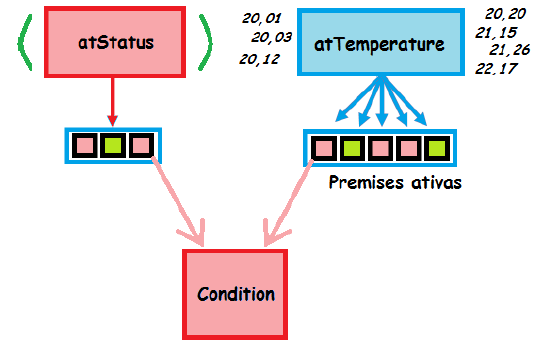
\includegraphics[width=0.55\textwidth]{../figures/pr_imp_1.png}
  \smallskip
  \caption{Alterações de estado com \textit{Attribute} impertinente ativo}
  \caption*{Fonte: \citeonline{msc_Ronszcka_2012}}
  \label{fig:pr_imp_1}
\end{figure}

Neste cenário em pauta, o \textit{Attribute} \textit{atTemperature} é
categorizado como impertinente por sua mudança estaticamente não aprovar a
\textit{Condition} da \textit{Rule}, logicamente em função da mudança largamente
mais discreta de seu parceiro de conjunção, o pertinente \textit{atStatus}.
Deste modo, para evitar notificações desnecessárias, suas \textit{Premises} não
deveriam receber notificações temporariamente, sendo que as notificações do
\textit{atTemperature} para tais \textit{Premises} seriam desabilitadas até
segunda ordem. A Figura \ref{fig:pr_imp_2} ilustra o mesmo cenário acima, porém
com \textit{atTemperature} sendo tido como um \textit{Attribute} impertinente
para com \textit{Premises}, tendo suas notificações temporariamente
desabilitadas.

\begin{figure}[!htb]
  \centering
  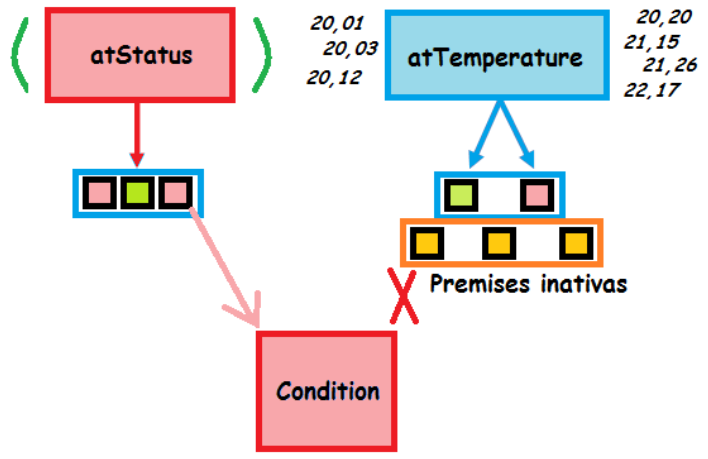
\includegraphics[width=0.55\textwidth]{../figures/pr_imp_2.png}
  \smallskip
  \caption{Alterações de estado com \textit{Attribute} impertinente desativado}
  \caption*{Fonte: \citeonline{msc_Ronszcka_2012}}
  \label{fig:pr_imp_2}
\end{figure}


Nesse âmbito a \textit{Condition} fica responsável por reativar temporariamente
as \textit{Premises} relativas a \textit{Attributes} impertinentes, de modo a
voltar receber notificações destas, quando o conjunto de \textit{Premises}
pertinentes para sua aprovação forem satisfeitas. Essa reativação temporária,
ilustrada na Figura \ref{fig:pr_imp_3}, torna capaz a aprovação da
\textit{Condition}. Por fim, após a aprovação e execução da \textit{Rule},
volta-se a desativar o \textit{Attribute} impertinente no contexto da
\textit{Rule} em questão. Desta forma, o \textit{Attribute} impertinente
voltaria a ignorar \textit{Premises} da \textit{Condition} daquela \textit{Rule}
até que fosse requisitado novamente pela \textit{Condition}
\cite{msc_Ronszcka_2012}.

\begin{figure}[!htb]
  \centering
  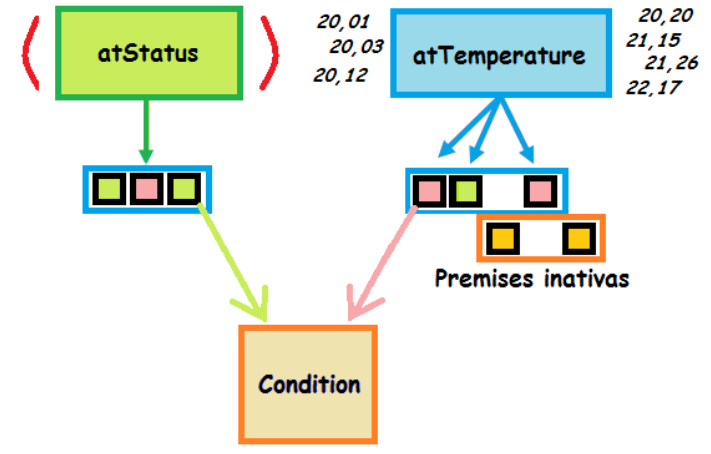
\includegraphics[width=0.55\textwidth]{../figures/pr_imp_3.png}
  \smallskip
  \caption{Alterações de estado com \textit{Attribute} impertinente reativado}
    \caption*{Fonte: \citeonline{msc_Ronszcka_2012}}
  \label{fig:pr_imp_3}
\end{figure}

\FloatBarrier

A definição de impertinência das entidades pode acontecer em dois momentos,
feita a priori ou em tempo de execução. Esses dois modos de impertinência são
chamados de impertinência estática e impertinência dinâmica. A impertinência
estática é de responsabilidade do desenvolvedor, de modo que a entidade já é
definida como impertinente no momento da compilação, enquanto a impertinência
dinâmica não é definida pelo desenvolvedor e sim por um mecanismo em tempo de
execução que seja capaz de detectar a impertinência das entidades a luz de dados
estatísticos.

\subsection{Compartilhamento de entidades}\label{sec:compartilhamento}

O uso do compartilhamento (de colaboração) de entidades pode ser considerado uma
boa prática do PON tanto da perspectiva da facilidade de desenvolvimento como
para o ganho de desempenho. O compartilhamento de entidades como
\textit{Conditions} e \textit{Premises} oferece ganhos de desempenho ao eliminar
a criação de estruturas redundantes e, com isso, também reduz o número de
notificações desnecessárias \cite{msc_Ronszcka_2012}. O ganho em facilidade de
desenvolvimento, por sua vez, é dado pelo fato do compartilhamento de entidades
acontecer de forma natural ao desenvolvedor durante o desenvolvimento das
\textit{Rules} do programa em PON. Quando o desenvolvedor escreve o código em
PON, seria um cenário comum diferentes \textit{Rules} estarem relacionadas às
mesmas \textit{Premises}, \textit{Conditions} ou \textit{Instigations}, as quais
seriam compartilhadas já em tempo de construção do programa.

O compartilhamento de entidades é um meio útil para a resolução do
problema de redundância estrutural, conceito introduzido na reflexão sobre
paradigmas da Seção \ref{sec:paradigmas}. Em suma, a redundância estrutural
ocorre, por exemplo, quando o conhecimento sobre um estado resultante da
avaliação de dada expressão lógica (\textit{e.g.}, comparação de uma variável com uma
constante) não é compartilhado entre outras expressões causais pertinentes,
causando reavaliações desnecessárias \cite{msc_Banaszewski_2009}. O
compartilhamento de colaboração de entidades evita avaliações redundantes, ao fornecer um meio
para se compartilhar os resultados das avaliações lógicas comuns a várias
expressões causais \cite{msc_Banaszewski_2009}.

\begin{figure}[!htb]
  \centering
  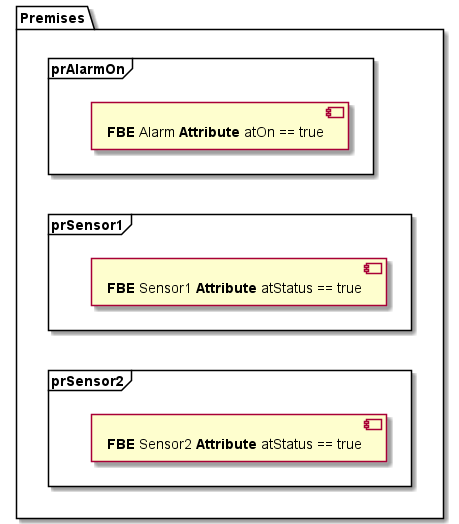
\includegraphics[width=0.45\textwidth]{../out/diagrams/shared_premises/premises.png}
  \smallskip
  \caption{Declaração de \textit{Premises} do exemplo do alarme}
  \caption*{Fonte: Autoria própria}
  \label{fig:premises_shared_ex}
\end{figure}

Para exemplificar o compartilhamento de entidades, é expandido o exemplo do
alarme, introduzido na Seção \ref{sec:estado_arte_pon}, para ter duas
\textit{Rules} e com dois \textit{FBEs} relativos aos sensores, porém apenas um
\textit{FBE} para o alarme. Neste caso, existem três \textit{Premises},
mostradas na Figura \ref{fig:premises_shared_ex}, e duas \textit{Rules},
mostradas na Figura \ref{fig:rules_shared_ex}. Nesse cenário observa-se que
ambas as \textit{Rules}, dependem da mesma \textit{Premise} \textit{prAlarmOn},
que neste caso é uma entidade cuja colaboração é compartilhada para com as
\textit{Rules}, sendo que ambas são notificadas pelas \textit{Premise} em
questão quando pertinente.

\begin{figure}[!htb]
  \centering
  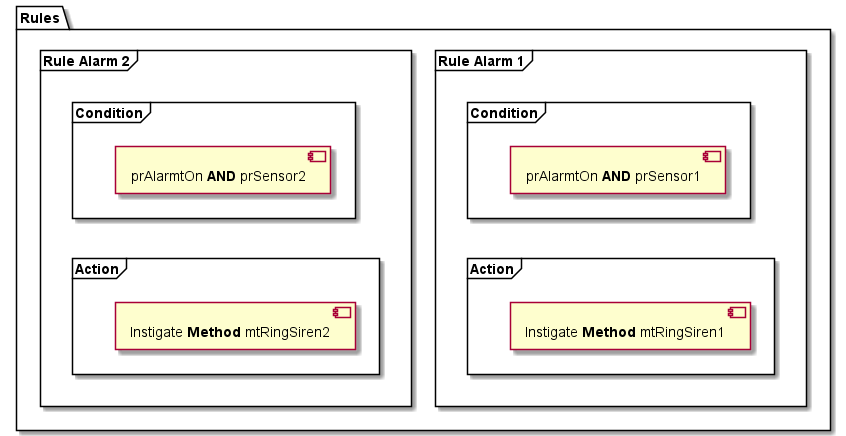
\includegraphics[width=0.8\textwidth]{../out/diagrams/rules_example/rules.png}
  \smallskip
  \caption{Declaração de \textit{Rules} utilizando \textit{Premises}
    compartilhadas}
  \caption*{Fonte: Autoria própria}
  \label{fig:rules_shared_ex}
\end{figure}

\subsection{Resolução de conflitos}\label{sec:conflitos}

Um conflito acontece quando duas atividades diferentes dependem de um mesmo
recurso compartilhado, o qual deve ser usado exclusivamente
\cite{doc_simao_2005}. Uma das características do PON é ser também orientado a
regras, sendo que conflitos entre regras podem surgir quando duas ou mais
\textit{Rules} são aprovadas com base em estado de recurso exclusivo. Outra
característica do PON é justamente permitir a execução de forma desacoplada e
concorrente dos elementos do seu modelo, permitindo paralelismos e distribuições
conforme o ambiente em que a aplicação PON seja executada. Nesse âmbito, é
importante a identificação e resolução de conflitos originados dessa execução
desacoplada de aprovação e execução de \textit{Rules} \cite{msc_pordeus_2017}.

No PON, mais precisamente, o conflito ocorre quando duas ou mais \textit{Rules}
referenciam um mesmo \textit{FBE} e demandam exclusividade de acesso a este
\textit{FBE} (como para o caso de modificar \textit{Attributes} deste
\textit{FBE}). Neste caso, apenas uma das \textit{Rules} poderia ser executada
por vez, fazendo o acesso exclusivo a este \textit{FBE}, o que leva ele a ser um
FBE exclusive neste contexto dado. Ainda, neste âmbito de conflitos, a resolução
de conflitos em ambientes monoprocessados ocorre de modo a estabelecer a ordem
de execução das \textit{Rules}. Já em ambientes multiprocessados, a resolução de
conflitos é necessária para evitar o acesso concorrente ao mesmo recurso
\cite{msc_valenca_2012,msc_Banaszewski_2009}.

Nos ambientes monoprocessados pode ser aplicado um escalonador de \textit{Rules}
que utiliza estruturas de dados lineares (\textit{e.g.}, pilha, filha ou lista)
\cite{msc_Banaszewski_2009}. Esse modelo, exemplificado na Figura
\ref{fig:conflitos}, recebe as \textit{Rules} na ordem em que são aprovadas e as
executa de acordo com a estratégia de resolução de conflito escolhida, o que
seria assaz similar a resolução conflitos em geral de sistemas baseados em
regras \cite{msc_Banaszewski_2009}. Isto dito, as diferentes estratégias de
resolução de conflitos para ambientes monoprocessados são listadas abaixo:

\begin{itemize}
  \item \textit{Breadth} ou largura: escalonamento \textit{First In First Out}
        (FIFO), primeiro a entrar é o primeiro a sair, no qual as \textit{Rules}
        são executadas na mesma ordem que são aprovadas. Pode ser usada uma
        estrutura de dados do tipo fila para este propósito.
  \item \textit{Depth} ou profundidade: escalonamento \textit{Last In First Out}
        (LIFO), último a entrar é o último a sair, no qual as \textit{Rules}
        são executadas começando sempre pela última \textit{Rule} aprovada. Pode
        ser usada uma estrutura de dados do tipo pilha para este propósito.
  \item \textit{Priority} ou prioridade: escalonamento baseado na prioridade definida para
        cada \textit{Rule}.
  \item \textit{No one} ou nenhum: a \textit{Rule} é executada imediatamente ao ser
        aprovada.
\end{itemize}

\begin{figure}[!htb]
  \centering
  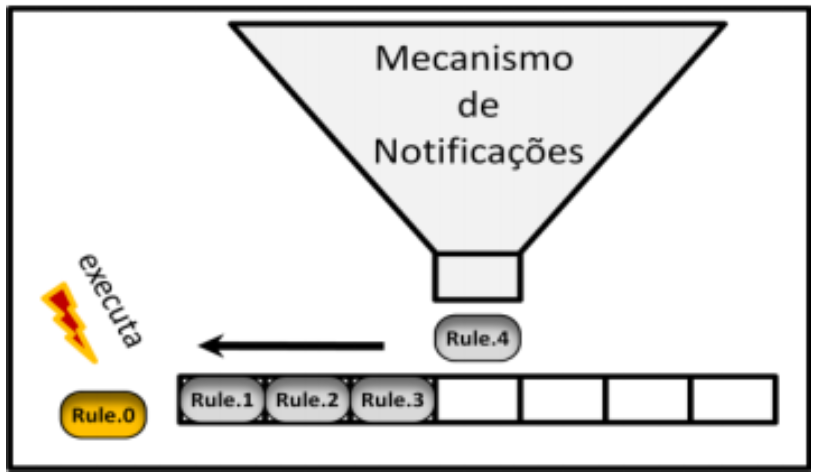
\includegraphics[width=0.7\textwidth]{../figures/conflitos.png}
  \smallskip
  \caption{Modelo centralizado de resolução de conflitos na estratégia
    \textit{Breadth}} \caption*{Fonte: \citeonline{msc_Banaszewski_2009}}
  \label{fig:conflitos}
\end{figure}

\FloatBarrier

Apesar deste modelo ser uma solução eficiente para ambientes monoprocessados,
ele não se mostra adequado para ambientes \textit{multicore} por não apresentar
um mecanismo que permita o escalonamento apropriado da execução das
\textit{Rules}. \citeonline{msc_Banaszewski_2009} então propõe tal mecanismo que
execute o escalonamento de forma eficiente. Para que este mecanismo de
escalonamento seja integrado ao modelo de resolução de conflitos, é necessário
alterar a forma pela qual as \textit{Rules} são executadas neste modelo. Assim, ao invés
de uma \textit{Rule} aprovada instigar a execução imediata da mesma, essa deve
repassar o controle da execução da respectiva \textit{Rule} para o componente
escalonador de \textit{Rules}. Quando a \textit{Rule} é aprovada, ao invés de ser
executada imediatamente, ela é adicionada a uma fila de execução, considerando a
prioridade de execução das respectivas \textit{Rules}. Por sua vez, essas
\textit{Rules} são executadas de forma escalonada por uma \textit{pool} de
executores, com um número de executores pré-definidos, que permite a execução
simultânea de múltiplas \textit{Rules}.

\subsection{\textit{Master Rule}}

Este conceito estabelece um mecanismo de dependência entre \textit{Rules}. Podem
existir cenários nos quais diferentes \textit{Rules} dependem do mesmo conjunto
de \textit{Premises} compartilhadas para sua aprovação, as quais notificariam
todas as entidades interessadas em suas mudanças de estado. Nesse caso as
notificações desnecessárias podem ser evitadas caso essas \textit{Premisses}
notifiquem uma única \textit{Rule}, ao invés de todas as interessadas. Essa
\textit{Rule}, quando aprovada, fica responsável por notificas as demais
\textit{Rules} interessadas e, portanto, dependentes daquela. Nesse cenário é
criada uma dependência entre as \textit{Rules}, na qual a \textit{Master Rule} é
capaz de notificar outras \textit{Rules} \cite{msc_Ronszcka_2012}. Esse
mecanismo traz benefícios em questões de desempenho e facilidade na composição
de aplicações, porque a dependência entre as \textit{Rules}, por meio do
conceito de \textit{Master Rule}, reduz as notificações geradas pelas
\textit{Premises} ao direcionar as notificações apenas para a \textit{Master
Rule} \cite{msc_Ronszcka_2012}.

Para exemplificar o conceito de \textit{Master Rule} é expandido o exemplo do
alarme explorado na Seção \ref{sec:compartilhamento}, com duas \textit{Rules} e
com dois \textit{FBEs} para os sensores, porém agora considerando que uma das
\textit{Rules}, chamada \textit{rlAlarm2}, depende de três \textit{Premises}
(\textit{prAlarmOn}, \textit{prSensor1} e \textit{prSensor2}), sendo que duas
destas \textit{Premises} fazem parte da composição de outra \textit{Rule},
chamada \textit{rlSensor1}, de modo que este cenário pode ser construído por
meio do uso de uma \textit{Master Rule}. Considere-se as mesmas três
\textit{Premises} da Figura \ref{fig:premises_shared_ex}, aplicadas nas
\textit{Rules} da Figura \ref{fig:master_rule}. Pela aplicação da \textit{Master
Rule}, a aprovação da \textit{rlAlarm2} só acontece após a \textit{rlAlarm1}
também ser aprovada.

\begin{figure}[!htb]
  \centering
  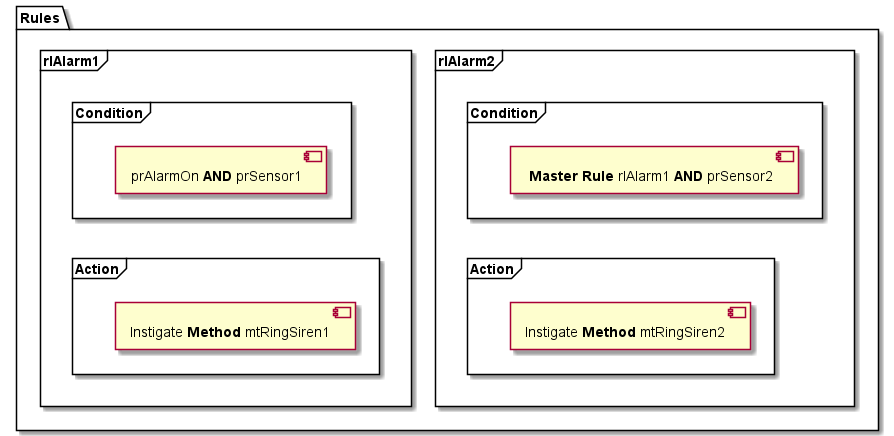
\includegraphics[width=0.8\textwidth]{../out/diagrams/master_rule/rules.png}
  \smallskip
  \caption{Exemplo de aplicação de \textit{Master Rule}}
  \caption*{Fonte: Autoria própria}
  \label{fig:master_rule}
\end{figure}

\subsection{\textit{Formation Rules} - Regras de Formação}

O conceito de \textit{Formation Rules} (ou Regra de Formação) do PON é um
reaproveitamento das \textit{Formation Rules} do Controle Orientado a
Notificações (CON), o predecessor do PON \cite{msc_simao_2001}. Cada
\textit{Formation Rule} permite a criação de \textit{Rules} específicas com base
na representação genérica de uma \textit{Rule}. Esse conceito é útil quando o
conhecimento causal de uma Rule é comum para diferentes conjuntos de instâncias
de \textit{FBEs}, ou seja, um conjunto de \textit{Rules} específicas se
diferencia apenas nas instâncias referenciadas \cite{doc_ronszcka_2019}.

A título de exemplo tome-se um cenário hipotético de um sistema de alarmes, no
qual existem as entidades usuários e alarmes (\textit{FBE User} e \textit{FBE
Alarm}). A responsabilidade do sistema seria de avisar cada usuário sobre a
ativação de cada alarme conectado. Para isso seria necessário replicar essa
condição para cada combinação de usuário e alarme (\textit{e.g.}, \textit{user1
x alarm1, user1 x alarm2, user2 x alarm1, user2 x alarm2 etc.}), o que torna o
processo custoso e propenso a erros \cite{doc_ronszcka_2019}.

Com a aplicação do conceito de \textit{Formation Rules} se torna possível a
declaração do conhecimento lógico-causal da \textit{Rule} de forma genérica, com
base nos tipos dos \textit{FBEs}, ao invés das instâncias pontuais de cada um.
Assim, em tempo de compilação, seria feita a composição das \textit{Rules} para
cada combinação de instâncias \cite{doc_ronszcka_2019}. Isso permite tornar a
replicação de \textit{Rules} uma tarefa automática, minimizando a possibilidade
de erros e facilitando o trabalho do desenvolvedor, além de promover maior
legibilidade do código em geral, ao remover a duplicação de código similar
repetido \cite{doc_ronszcka_2019}.

A Figura \ref{fig:formation_rule} ilustra uma representação de uma
\textit{Formation Rule} que pode ser adotada para gerar as instâncias das
\textit{Rules} referentes a um cenário de automatização do controle de veículos.
Neste caso a \textit{Formation Rule} define a \textit{Rule} que deve ser
aplicada a todos os carros e cruzamentos, onde o veículo só pode acelerar caso o
sinal esteja no estado verde e não hajam pessoas andando no cruzamento.

\begin{figure}[!htb]
  \centering
  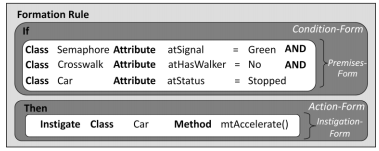
\includegraphics[width=0.7\textwidth]{../figures/formation_rule.png}
  \smallskip
  \caption{Representação de uma \textit{Formation Rule}}
  \caption*{Fonte: \citeonline{msc_Banaszewski_2009}}
  \label{fig:formation_rule}
\end{figure}

Uma \textit{Formation Rule} é mais genérica do que uma \textit{Rule}
tradicional. Para sua descição é utilizado o sufixo \textit{Form}, que define as
lógicas que é utilizada como base para instanciar de forma efetiva cada uma das
entidades do PON. As suas entidades \textit{Form} somente analisam se o
\textit{FBE} é de uma determinada classe. Uma \textit{Formation Rule} filtra e
cria combinações de \textit{FBEs}, onde cada combinação resulta na criação de
uma \textit{Rule} independente. Em suma, uma \textit{Formation Rule} aplica
conceitos genéricos a fim de criar \textit{Rules} específicas, mantendo a
capacidade de notificação entre os objetos colaboradores. A função principal da
\textit{Formation Rule} é gerar automaticamente a partir de um modelo várias
instâncias de Rules que compartilham a semântica deste modelo. 


\subsection{\textit{FBE Rules}}\label{sec:fbe_rule}

De maneira geral, o conceito de agregações de \textit{Rules} em \textit{FBEs} é
um conceito próximo ao das \textit{Formation Rules}, sendo um caso particular
das \textit{Formation Rules} no qual a \textit{Rule} está relacionada a apenas
um tipo de \textit{FBE}, enquanto nas \textit{Formation Rules} a \textit{Rule}
pode estar relacionada a vários \textit{FBE} \cite{msc_santos_2017}. Uma
\textit{FBE Rule} é uma \textit{Rule} que possui escopo local em seu
\textit{FBE}, e todas as instâncias deste \textit{FBE} possuem,
obrigatoriamente, uma instância da \textit{Rule} em questão
\cite{doc_ronszcka_2019}.

A título de exemplo considera-se a aplicação do alarme com seu respectivo
sensor. Para a execução de vários alarmes seria necessário replicar as
\textit{Rules} para cada instância. Porém, com a utilização do conceito de
\textit{FBE Rules}, essa replicação pode ser feita de modo automático com a
declaração da \textit{Rule} como uma \textit{FBE Rule} do \textit{FBE} do
alarme. A Figura \ref{fig:fbe_rule} ilustra este cenário.

\begin{figure}[!htb]
  \centering
  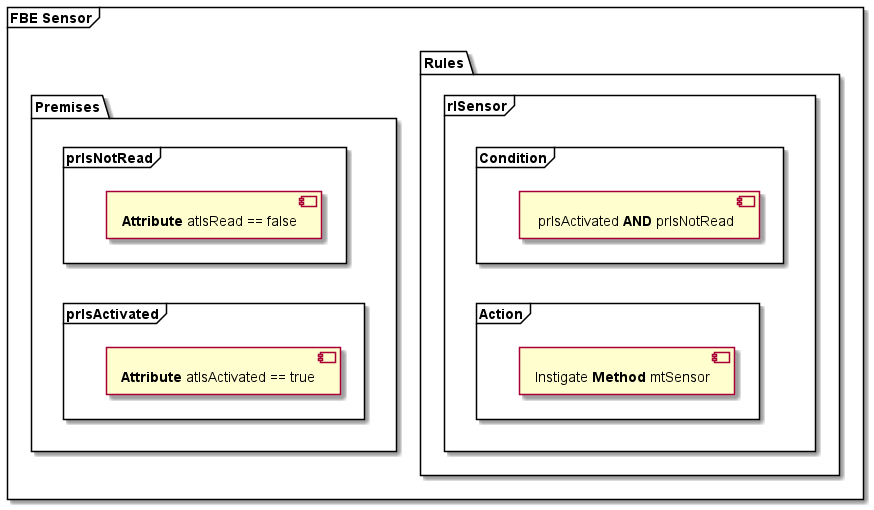
\includegraphics[width=0.8\textwidth]{../out/diagrams/fbe_rule/rules.png}
  \smallskip
  \caption{Exemplo de aplicação de \textit{FBE Rules}}
  \caption*{Fonte: Autoria própria}
  \label{fig:fbe_rule}
\end{figure}

\subsection{Agregação entre \textit{FBEs}}\label{sec:agregacao}

Outro conceito pertinente ao PON é possibilidade de criar agregações entre
\textit{FBEs}, permitindo a criação de \textit{FBEs} compostos sem a necessidade
de duplicação de estruturas. Esse conceito permite otimizações na redução de
código, assim como também facilita a descrição de programas em PON, tanto de
forma textual como gráfica \cite{doc_ronszcka_2019}. Com isso, espera-se atingir
níveis de organização mais efetivos, melhorando particularmente a escrita e a
legibilidade de programas baseados no PON.

Esta forma de estruturação facilita a construção de \textit{Rules} que podem ser
compostas internamente aos \textit{FBEs}, sendo o caso das \textit{FBE Rules}.
Neste caso a agregação de \textit{FBEs} permite a criação de \textit{Rules}
utilizando todos os \textit{FBEs} agregados. 

%Como no caso do exemplo da Seção \ref{sec:fbe_rule}, no qual o \textit{FBE}
%\textit{Alarm} agrega o \textit{FBE} Sensor, de forma que cada instância do
%\textit{FBE Alarm} cria uma instância do seu \textit{FBE Sensor} agregado.

\subsection{Resumo dos Conceitos de Programação do PON}

Nas seções anteriores foram apresentados diversos conceitos de programação do
PON. De forma a facilitar o entendimento sobre tais conceitos, a Tabela
\ref{tab:resumo_conceitos} apresenta um resumo de cada um desses conceitos.
Isto é feito de forma a apresentar de forma simplificada e centralizada o
conhecimento sobre os conceitos de programação do PON.

É importante ressaltar que apesar de todas as materializações do PON buscarem
aplicar todos esses conceitos, raramente isso acontece. Alguns conceitos de
programação foram introduzidos por materializações mais recentes do PON, de modo
que, naturalmente, as implementações que precedem a introdução de determinado
conceito não o materializam. Ainda assim, mesmo em materializações mais recentes,
limitações de ordem técnica ou conceitual podem impedir a implementação de todos
esses conceitos.

\begin{table}[!htb]
\centering
\caption{Resumo de conceitos de programação do PON}
\caption*{Fonte: Autoria própria}
\label{tab:resumo_conceitos}
\begin{tabularx}{\textwidth}{l|X}
Conceito                              & Definição                                                                                                                                  \\ \hline\hline
Reatividade das entidades             & Entidades são capazes de gerar notificações pontuais de forma espontânea na alteração de estado                                            \\ \hline
Renotificações                        & Entidades podem gerar notificações de forma forçada, mesmo sem alteração nos seus estados                                                  \\ \hline
\textit{Keeper}                       & Controle manual de execução das \textit{Rules}, permitindo execução de uma \textit{Rule} múltiplas vezes enquanto aprovada                 \\ \hline
Impertinência                         & Supressão seletiva de notificações de determinadas entidades, podendo ocorrer de forma estática ou dinãmica                                \\ \hline
Compartilhamento de entidades         & Utillização compartilhada de entidades com conhecimento em comum com outras entidades, reduzindo o número de entidades únicas no sistema   \\ \hline
\textit{Master Rule}                  & Relação de depedência entre \textit{Rules} com conhecimento lógico-causal em comum                                                         \\ \hline
\textit{Formation Rules}              & Criação de \textit{Rules} baseadas na representação genérica de uma \textit{Rule} relativa ao tipo dos \textit{FBEs}                       \\ \hline
\textit{FBE Rules}                    & Definição de \textit{Rules} no corpo do \textit{FBE}, instanciando uma \textit{Rule} independente para cada instância de dado \textit{FBE} \\ \hline
Agregação entre \textit{FBEs}         & Criação de \textit{FBEs} compostos de outros \textit{FBEs}                                                                                 \\ \hline
\end{tabularx}
\end{table}

\clearpage
\section{Materializações do PON em software}\label{sec:frameworks}

O PON apresenta materializações tanto em software quanto em hardware
\cite{doc_linhares_2015,doc_Kerschbaumer_2018,doc_ronszcka_2019,doc_Schutz_2019}.
Entretanto, este trabalho foca nas implementações em software e não hardware.
Nas implementações em software, há tanto implementações em \textit{frameworks}
como também por meio de linguagem de programação própria, por meio da chamada
Tecnologia LingPON. Enquanto a linguagem de programação via Tecnologia LingPON
se constitui em estado da arte por ainda ser consideravelmente prototipal, o
conjunto de \textit{frameworks} se constituem no estado da técnica por parte
deles se encontrar em estado estável de desenvolvimento.

As implementações por meio de \textit{frameworks} existem de forma a oferecer
uma interface de programação de aplicativos (API - \textit{Application
Programming Interface}) que possibilite o desenvolvimento de aplicações seguindo
o modelo do PON, modificando, portanto, a maneira como estas linguagens operam,
justamente permitindo e conduzindo-lhes a operarem de forma orientada a
notificações. As seções seguintes apresentam cada uma destas materializações em
software em maiores detalhes, sendo que a primeira subseção desta presente seção
se dedica aos \textit{frameworks} para o PON desenvolvidos em linguagem de
programação C++.

\subsection{\textit{Frameworks} PON C++}

A materialização do PON em C++ conta com mais de uma única implementação, sendo
que cada uma destas materializações foi construída com base nas materializações
anteriores, cada uma com sua proposta de melhoria específica. Estas diferentes
materializações são o \textit{Framework} PON C++ Prototipal, \textit{Framework}
PON C++ 1.0, \textit{Framework} PON C++ 2.0 e \textit{Framework} PON C++ 3.0.
Além dessas materializações, também há o prototipal JuNOC++, desenvolvido por
\citeonline{chierichi_2020} com base no trabalho da dissertação de
\citeonline{msc_Ronszcka_2012}. Estas materializações são exploradas
individualmente em maior detalhe nas seções seguintes.

%\footnote{Também há a implementação
%do \textit{Framework} JuNOCpp, desenvolvido por Gustavo Chierici, como uma
%reimplementação do \textit{Framework} PON C++ 2.0, com base no trabalho da
%dissertação de mestrado do Ronszcka em 2012, disponível em
%\url{https://github.com/GustavoChierici/JuNOCpp}}

\subsubsection{\textit{Framework} PON C++ Prototipal}\label{sec:fw_prot}

A primeira implementação do PON sobre o formato de \textit{framework}, o chamado
\textit{Framework} PON C++ Prototipal, foi proposta por Simão em 2007
\cite{pat_simao_2008,simao_2012a}. Esta versão prototipal do \textit{framework}
deriva dos esforços de sua dissertação de mestrado e tese de doutorado no âmbito
do metamodelo do Controle Orientado a Notificações (CON), o qual foi aplicado
sobre a ferramenta de simulação de sistema de manufatura ANALYTICE II
\cite{doc_simao_2005,simao_2009}.

A Figura \ref{fig:mira_alvo} é apresentada com o objetivo de ilustrar uma
aplicação desenvolvida com a aplicação do \textit{Framework} PON C++ Prototipal.
Neste exemplo de implementação, toma-se uma aplicação intitulada Mira ao Alvo,
na qual as entidades miras e as entidades alvos são representadas
respectivamente por arqueiros e maçãs, sendo que há uma maçã para cada arqueiro.
Isto dito, este cenário é descrito sob a forma de \textit{FBEs} e \textit{Rule}
no Código \ref{cod:mira_alvo_fbe}.

\noindent
\begin{minipage}{.45\textwidth}
  \centering
  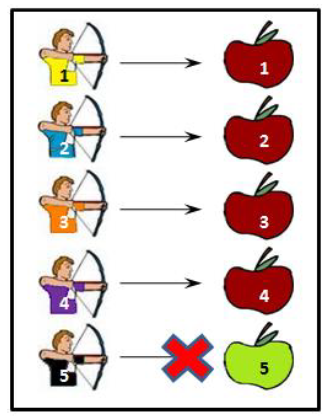
\includegraphics[width=.8\textwidth]{../figures/mira_alvo.png}
  \captionof{figure}{Cenário do Mira ao Alvo}
  \captionof{figure}*{Fonte: \citeonline{msc_Banaszewski_2009}}
  \label{fig:mira_alvo}
\end{minipage}\hfill
\begin{minipage}{.45\textwidth}
  \begin{lstlisting}[caption = {\textit{FBEs} e \textit{Rule} para cenário do Mira ao Alvo},
    source = {\citeonline{chierichi_2020}}, language=nopl,
    label = {cod:mira_alvo_fbe}]
fbe Archer
  public boolean atStatus = false
  public integer atIdentity = 0
end_fbe
fbe Apple
  public boolean atAppleColor = false
  public integer atIdentity = 0
  public boolean atIsCrossed = false
  private method mtStatusOff
    attribution
      this.atIsCrossed = true
    end_attribution
  end_method
end fbe
inst
 Archer archer
 Apple apple
end_inst

rule rlShootApple
  condition
      premise prIdentity
        apple.atIdentity == archer.atIdentity
      end_premise
      and
      premise prColor
        apple.atColor == true
      end_premise
      and
      premise prAppleStatus
        apple.atStatus == true
      end_premise
      and
      premise prArcherStatus
        archer.atStatus == true
      end_premise
      and
      premise prAppleIsNotCrossed
        apple.atIsCrossed == false
      end_premise
  end_condition
  action sequential
      instigation sequential
        call apple.mtStatusOff()
      end_instigation
  end_action
end_rule
  \end{lstlisting}
\end{minipage}

Em termos de implementação, no \textit{Framework} PON C++ Prototipal, cada
arqueiro e maçã é representado por um objeto notificante na forma de FBE
(\textit{i.e.}, um Elemento da Base de Fatos), os quais interagem de acordo com
a avaliação de expressões causais pertinentes na forma de objetos \textit{Rules}
(\textit{i.e.}, uma \textit{Rule}) \cite{msc_Banaszewski_2009}. Essa
implementação em foco é mostrada no Código \ref{cod:fwprot_ex}.

\begin{lstlisting}[caption = {Exemplo de programa com o \textit{framework} C++ prototipal},
  source = {Adaptado de \citeonline{msc_Banaszewski_2009}},
  label = {cod:fwprot_ex}, float=htb]
//Premises
prAppleColorRead = new AgentePremissa(appleList->at(i)->atAppleColor, True);
prAppleColorRead->conectaPredBooleano(&comparaBooleanos);
prAppleStatusTrue = new AgentePremissa(appleList->at(i)->atAppleStatus, True);
prAppleStatusTrue->conectaPredBooleano(&comparaBooleanos);
prArcherStatusTrue = new AgentePremissa(archerList->at(i)->atArcherStatus, True);
prArcherStatusTrue->conectaPredBooleano(&comparaBooleanos);
//Conditions
AgenteCondicao* cdFireApple;
acFireApple = new AgenteAcao();
acFireApple->conectaAgenteOrdem(appleList->at(i)->mtChangeToGreen);
//Method
mtChangeToGreen = new AgenteMetodoGen<Apple>(&Apple::ChangeToGreen);
//Instigation
aitChangeToGreen = new AgenteOrdem(mtChangeToGreen);
//Rule
AgenteRegra* rlFireApple;
rlFireApple = new AgenteRegra(cdFireApple, acFireApple);
\end{lstlisting}

\vspace{-1cm}
\subsubsection{\textit{Framework} PON C++ 1.0}

O \textit{Framework} PON C++ 1.0 foi implementado por Banaszewski em 2009, com a
proposta de facilitar e melhorar a composição de programas em PON. A estrutura
de implementação desta versão do \textit{framework} é constituída por dois
principais pacotes de classes, o pacote \textit{Core} e o pacote
\textit{Application}, conforme ilustrado na Figura \ref{fig:fw_pkg}. O pacote
\textit{Core} contém as classes que modelam as entidades do metamodelo do PON,
enquanto o pacote \textit{Application} contém as classes utilizadas para a
instanciação de uma aplicação em PON, usando as entidades do pacote
\textit{Core} \cite{msc_Banaszewski_2009}.

\begin{figure}[!htb]
  \centering
  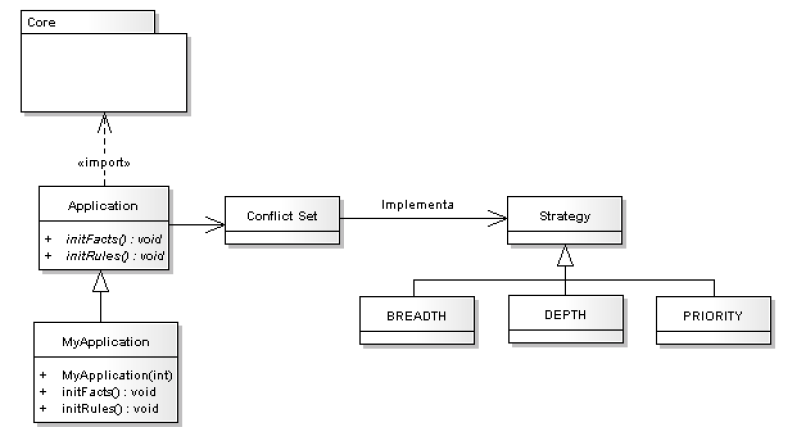
\includegraphics[width=0.85\textwidth]{../figures/fw1_structure.png}
  \caption{Estrutura do \textit{framework} C++ 1.0} \caption*{Fonte:
    \citeonline{msc_Banaszewski_2009}}
  \label{fig:fw_pkg}
\end{figure}

Nesta estrutura, a classe \textit{MyApplication} é um exemplo de implementação
que seria definida pelo programador com base na classe abstrata
\textit{Application} do \textit{framework}. A classe \textit{Application}
representa um modelo de inicialização padrão para aplicações em PON, por meio da
construtora da classe, na qual é definida a estratégia de resolução de
conflitos, bem como dos métodos \textit{initFacts} e \textit{initRules}, os
quais são respectivamente usados para concentrar a instanciação dos
\textit{FBEs} e \textit{Rules} \cite{msc_Banaszewski_2009}.

Em resumo, a construção de aplicações utilizando o \textit{Framework} PON C++
1.0 se baseia em torno da especialização da classe \textit{Application}, que
contém os métodos necessários para a inicialização das estruturas do PON. Um
exemplo de aplicação para o mesmo cenário Mira ao Alvo, já descrito
anteriormente na Seção \ref{sec:fw_prot}, agora com o \textit{framework} C++
1.0, é mostrado no Código \ref{cod:fw1_ex}.

\begin{lstlisting}[caption = {Exemplo de programa com o \textit{framework} C++ 1.0},
source = {Adaptado de \citeonline{msc_Banaszewski_2009}},
   label = {cod:fw1_ex}, float=htb]
for ( iteratorArcher = archerList->begin(), iteratorApple = appleList->begin(); 
      iteratorArcher != archerList->end();
      ++iteratorArcher, ++iteratorApple)
{	
  Instigation* it = new Instigation((*iteratorApple)->mtStatusOff);
  RuleObject* rlFireApple = new RuleObject("",scheduler, Condition::CONJUNCTION);

  rlFireApple->addPremise((*iteratorApple)->atIdentity,
                          (*iteratorArcher)->atIdentity, Premise::EQUAL, false);
  rlFireApple->addPremise((*iteratorApple)->atAppleColor,
                          Boolean::TRUE_NOP, Premise::EQUAL, false);
  rlFireApple->addPremise((*iteratorApple)->atAppleStatus,
                          Boolean::TRUE_NOP, Premise::EQUAL, false);
  rlFireApple->addPremise((*iteratorApple)->atAppleIsCrossed,
                          Boolean::FALSE_NOP, Premise::EQUAL, false);
  rlFireApple->addPremise((*iteratorArcher)->atArcherStatus,
                          Boolean::TRUE_NOP, Premise::EQUAL, false);
  rlFireApple->addPremise(gun->atIsFired,
                          Boolean::TRUE_NOP, Premise::EQUAL, false);
  rlFireApple->addPremise(gun->atIdentityOfBullet,
                          cont, Premise::EQUAL, false);

  rlFireApple->addInstigation(it);
  rlFireApple->end();
  cont++;
}
\end{lstlisting}

Isto dito, com as melhorias propostas, foi possível obter ganhos de desempenho
quando comparado o \textit{Framework} PON C++ 1.0  para com o \textit{Framework}
PON C++ prototipal. Para avaliar o desempenho destas duas versões foi executada
a aplicação do cenário Mira ao Alvo, variando a porcentagem de \textit{Rules}
aprovadas em cada iteração, no qual a aplicação com o \textit{Framework} PON C++
1.0 chega a atingir tempos de execução 60\% menores que os da aplicação com o
\textit{Framework} PON C++ prototipal. Na Figura \ref{fig:fw1_vs_prot} é
mostrado o resultado para a execução de 10.000 iterações, nela \enquote{Versão Antiga}
se refere ao \textit{framework} C++ Prototipal e \enquote{Versão Nova} se refere ao
\textit{framework} C++ 1.0 \cite{msc_Banaszewski_2009}.

\begin{figure}[!htb]
  \centering
  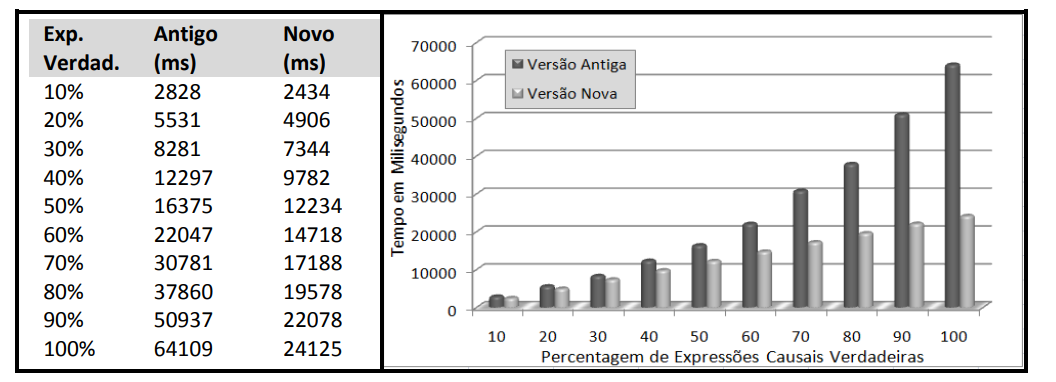
\includegraphics[width=\textwidth]{../figures/fw1_vs_prot.png}
  \caption{Comparação do desempenho do \textit{framework} C++ 1.0 com o
  \textit{framework} C++ Prototipal} \caption*{Fonte:
  \citeonline{msc_Banaszewski_2009}}
  \label{fig:fw1_vs_prot}
\end{figure}

\FloatBarrier

\subsubsection{\textit{Framework} PON C++ 2.0}\label{sec:fw2_revisao}

Subsequentemente, uma nova versão do \textit{framework} foi introduzida a partir
dos esforços de trabalhos de mestrado de Valença e Ronszcka em 2012
\cite{msc_valenca_2012,msc_Ronszcka_2012}. A estrutura da versão 2.0, ilustrada
na Figura \ref{fig:fw2_struct}, ainda mantém uma estrutura muito similar àquela
introduzida na versão 1.0, adotando a mesma estrutura de pacotes
\cite{msc_Ronszcka_2012}. Essa versão é considerada a principal materialização
estável para o desenvolvimento de aplicações no PON, por possuir o maior grau de
maturidade e estabilidade entre as materializações existentes para implementação
do PON em \textit{software} \cite{doc_ronszcka_2019}.

\begin{figure}[!htb]
  \centering
  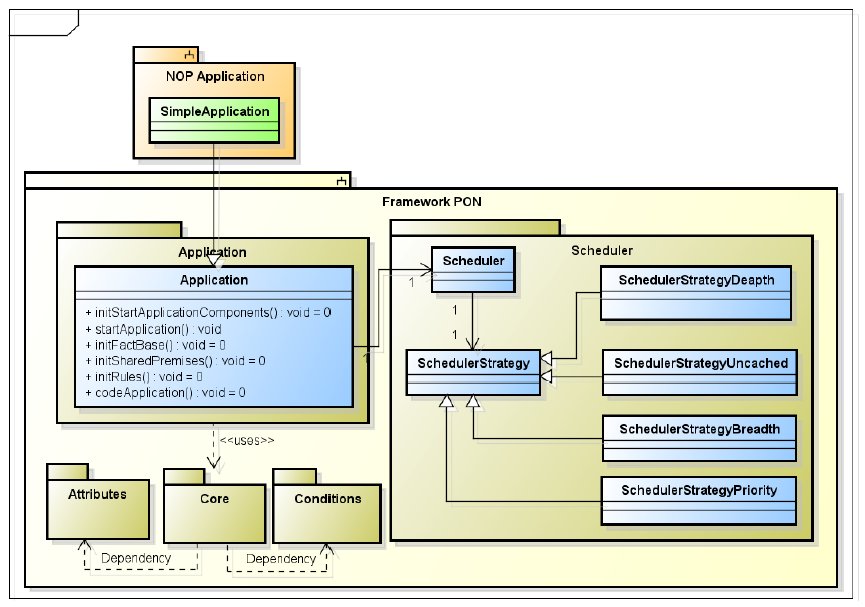
\includegraphics[width=0.9\textwidth]{../figures/fw2_structure.png}
  \caption{Estrutura do \textit{framework} C++ 2.0} \caption*{Fonte:
    \citeonline{msc_valenca_2012}}
  \label{fig:fw2_struct}
\end{figure}

Nesta implementação, Ronszcka propôs a utilização de padrões de projeto para o
desenvolvimento do \textit{framework} \cite{msc_Ronszcka_2012}, enquanto Valença
efetuou 'otimizações' (\textit{i.e.}, aprimoramentos) por meio do uso de
estruturas de dados com implementação própria (nomeadamente \textit{NOPVECTOR},
\textit{NOPHASH} e \textit{NOPLIST}), com melhor desempenho computacional que as
estruturas da STL. Com as melhorias propostas, foi possível obter ganhos de
desempenho quando comparado o Framework PON C++ 2.0 com o \textit{Framework} PON
C++ 1.0 \cite{msc_valenca_2012}. 

Ainda, com base nesta versão de \textit{framework}, foi desenvolvida uma aplicação
gráfica que possibilita a criação de \textit{FBEs} e \textit{Rules}, chamada
\textit{Wizard} PON, a qual é mostrada na Figura \ref{fig:wizard}. Com o auxílio
dessa aplicação é possível fazer a construção de um programa em PON em alto
nível, de maneira visual. Com essa ferramenta é possível escrever a estrutura do
programa em PON que passa então por um processo de geração de código para o
\textit{Framework} PON C++ 2.0 \cite{msc_valenca_2012}.

\begin{figure}[!htb]
  \centering
  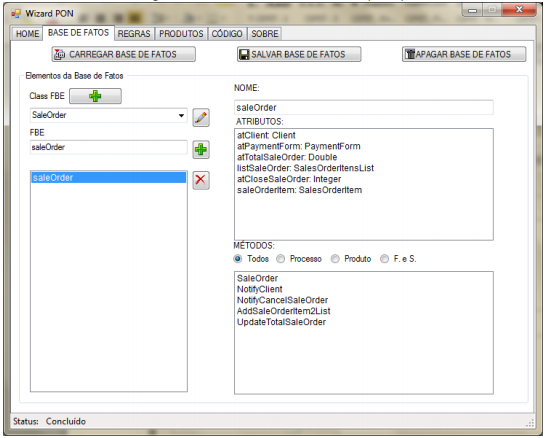
\includegraphics[width=.9\textwidth]{../figures/wizard.png}
  \caption{\textit{Wizard} PON} \caption*{Fonte: \citeonline{msc_valenca_2012}}
  \label{fig:wizard}
\end{figure}

Um exemplo de aplicação para o mesmo cenário Mira ao Alvo, já descrito
anteriormente na Seção \ref{sec:fw_prot}, mas agora com o \textit{Framework} PON
C++ 2.0 é mostrado no Código \ref{cod:fw2_ex}. Nota-se a sintaxe bastante
similar à do \textit{Framework} PON C++ 1.0, porém com a adição do uso do padrão
de projeto \textit{factory}. 

\begin{lstlisting}[caption = {Exemplo de programa com o \textit{framework} C++ 2.0},
source = {Adaptado de \citeonline{msc_valenca_2012}},
  label = {cod:fw2_ex}, float=htb]
Premise* p = elementsFactory->createPremise(gun->atIsFired, true, Premise::EQUAL, false);
for ( int i = 0; i < appleList->size(); i++ ){
  Apple* appleTmp = appleList->at(i);
  Archer* archerTmp = archerList->at(i)

  RuleObject* rlFireApple = elementsFactory->createRuleObject(
                              "rule", scheduler, Condition::CONJUNCTION);
  rlFireApple->addPremise(
    elementsFactory->createPremise(
      appleTmp->atIdentity,archerTmp->atIdentity, Premise::EQUAL, false));
  rlFireApple->addPremise(
    elementsFactory->createPremise(
      appleTmp->atAppleColor, true, Premise::EQUAL, false));
  rlFireApple->addPremise(
    elementsFactory->createPremise(
      appleTmp->atAppleStatus, true, Premise::EQUAL, false));
  rlFireApple->addPremise(
    elementsFactory->createPremise(
      appleTmp->atAppleIsCrossed, false, Premise::EQUAL, false));
  rlFireApple->addPremise(
    elementsFactory->createPremise(
      archerTmp->atArcherStatus, true, Premise::EQUAL, false));
  rlFireApple->addPremise(p);
  rlFireApple->addInstigation(
    elementsFactory->createInstigation(appleTmp->mtStatusOff));
}
\end{lstlisting}

\FloatBarrier

A mesma aplicação Mira ao Alvo é utilizada para comparar o desempenho do
\textit{Framework} PON C++ 2.0 com o \textit{framework} C++ 1.0. Nestes testes, a
utilização do \textit{Framework} PON C++ 2.0 foi com a estrutura de dados
\textit{PONVECTOR} apresentou em média 30\% do tempo de processamento utilizado
em relação ao \textit{Framework} PON C++ 1.0, o que corresponderia a um ganho de
desempenho de cerca três vezes, conforme observado na Figura
\ref{fig:fw2_vs_fw1}. Nessa figura \enquote{\textit{Framework} Original} se refere  ao
\textit{Framework} PON C++ 1.0.

\begin{figure}[!htb]
  \centering
  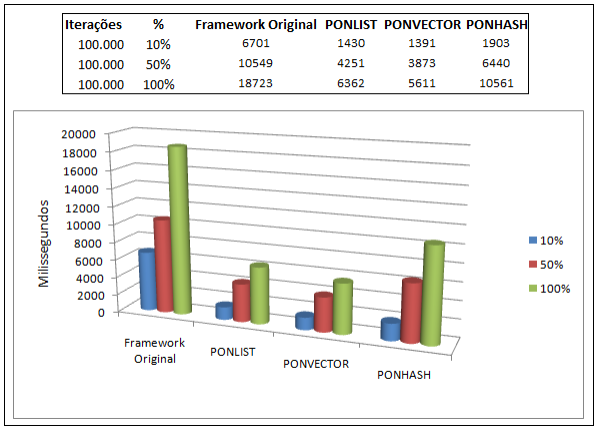
\includegraphics[width=0.8\textwidth]{../figures/fw2_vs_fw1.png}
  \caption{Comparação do desempenho do \textit{Framework} PON C++ 2.0 com o
  \textit{Framework} PON C++ 1.0}
  \caption*{Fonte: \citeonline{msc_valenca_2012}}
  \label{fig:fw2_vs_fw1}
\end{figure}

\subsubsection{\textit{Framework} PON C++ 3.0}\label{sec:fw3}

Tanto a versão do \textit{Framework} PON C++ 1.0 como o \textit{Framework} PON
C++ 2.0 consideram apenas a execução em ambientes monoprocessados e
monoprocesso/\textit{single thread} em sua concepção. Ou seja, \textit{Frameworks}
PON C++ 1.0 e 2.0 não consideram execução em ambiente \textit{multithread},
multiprocesso e, menos ainda, \textit{multicore}. Nesse sentido, foi proposto o
\textit{Framework} PON C++ 3.0. Esta versão é uma extensão da implementação do
\textit{Framework} PON C++ 2.0 incluindo a execução de conjuntos de
\textit{Rules} por meio de \textit{threads} independentes. Ademais, ele fornece
uma maneira de se paralelizar elementos do PON de forma transparente, em nível
de \textit{thread} para ambientes \textit{multicore} \cite{belmonte_2012}.

A estrutura do \textit{Framework} PON C++ 3.0 é apresentada na Figura
\ref{fig:fw3_struct}. Nela, os pacotes \textit{Application} e \textit{Core} são
os mesmos do \textit{Framework} PON C++ 2.0. Ainda com base nessa figura e na
Figura \ref{fig:fw2_struct}, podem ser destacadas algumas diferenças. Dentre
elas, há a criação do \textit{NOPVectorMulticore}, uma especialização do
\textit{NOPVECTOR} desenvolvido especialmente para trabalhar com aplicações
\textit{multicore}, agindo como um iterador das entidades do PON de forma
otimizada, reduzindo o uso do \textit{cache} da aplicação
\cite{belmonte_2012,schutz_2018}. Também há a adição do pacote
\textit{Multicore}, cujas entidades são detalhadas abaixo:

\begin{itemize}
  \item \textit{SynchronizedQueue}: Fila que armazena as entidades do PON a
        serem executadas, de forma sincronizada, em cada \textit{core} do
        processador \cite{belmonte_2012,schutz_2018}.
  \item \textit{CoreController}: Classe responsável por enfileirar as entidades
        do PON quando o \textit{CoreControllersManager} registra uma
        notificação. Também é responsável pela execução paralelizada das
        \textit{Premises}, \textit{Conditions} e \textit{Methods} em cada
        \textit{core} \cite{belmonte_2012,schutz_2018}.
  \item \textit{CoreControllersManager}: Classe responsável por criar a
        instância do \textit{CoreController} para cada \textit{core} do
        processador. Durante a execução responsável por registrar as
        notificações recebidas pelas entidades do PON \cite{belmonte_2012,schutz_2018}.
  \item \textit{Thread}: Classe de execução que controla o uso das
        \textit{threads}, por meio do uso de mecanismos de exclusão mútua. Para
        sua implementação é utilizada a biblioteca \textit{pthreads}
        \cite{belmonte_2012,schutz_2018}.
  \item \textit{SleepCondition}: Classe que possui métodos para auxiliar o
        controle da execução da fila de entidades do PON. Para sua implementação
        é utilizada a biblioteca \textit{pthreads} \cite{belmonte_2012,schutz_2018}.
\end{itemize}

Conforme descrito acima à luz da Figura \ref{fig:fw3_struct}, novas classes
foram criadas para suportar o mecanismo \textit{multithread} e usar paralelismo
em nível de \textit{thread} quando em um contexto de dois ou mais núcleos ou
\textit{cores} (\textit{multicores}), utilizando inclusive a API \textit{pthreads}. Esta
API fornece um conjunto de bibliotecas com recursos de controle e sincronização
de \textit{threads}, por meio dos conceitos de exclusão mútua (\textit{mutex})
para controlar o acesso e a execução de entidades compartilhadas entre as
\textit{threads}.

\begin{figure}[!htb]
  \centering
  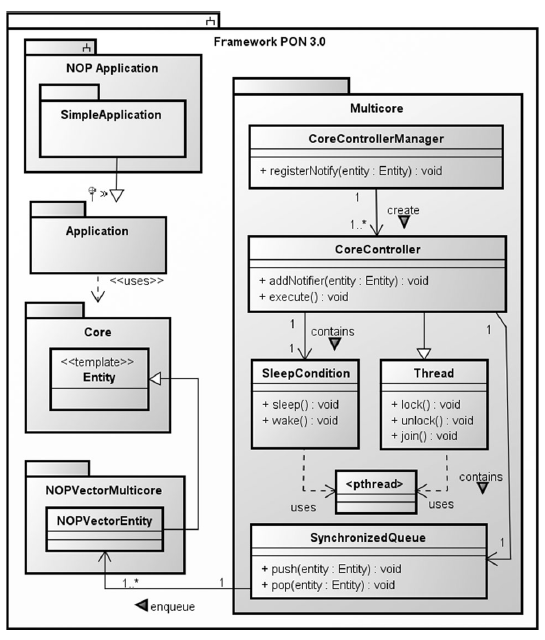
\includegraphics[width=.65\textwidth]{../figures/fw_30.png}
  \caption{Estrutura do \textit{framework} C++ 3.0} \caption*{Fonte:
    \citeonline{schutz_2018}}
  \label{fig:fw3_struct}
\end{figure}

A classe \textit{CoreControllermanager} é responsável por instanciar cada
\textit{FBE} da aplicação em um núcleo específico, de forma que as entidades da
cadeia de notificações sejam distribuídas entre os núcleos disponíveis de forma
controlada \cite{doc_Schutz_2019}. A fim de respeitar a execução correta das
entidades PON em cada núcleo, a classe \textit{CoreController} gerencia uma fila
de entidades a serem executadas, a \textit{SynchronizedQueue}. Assim, uma
entidade notificada vai para esta fila de execução e, assim que um núcleo do
processador esteja disponível, uma entidade é removida da fila e executada,
segundo o processo ilustrado na Figura \ref{fig:fw3_flow}

Além disso, durante o desenvolvimento do \textit{Framework} PON C++ 3.0
persebeu-se a existência de um problema de \textit{stack overflow} (estouro de
pilha), possívelmente presente em todos os \textit{frameworks} em C++
anteriores. O \textit{stack overflow} acontece quando ocorre a chamada de muitas
funções em sequência, sem nunca retornar, o que pode ser causado, por exemplo,
por uma sequência muito grande de notificações que realimenta o ciclo de
notificações indefinidamente. Subsequentemente no \textit{Framework} PON C++ 3.0
foi criado um desacoplamento do mecanismo de notificações, onde o
\textit{Method} não é instigado diretamente pela entidade notificante, mas sim
colocada dentro de uma fila de notificações dentro de uma entidade controladora,
o \textit{CoreController}, quebrando assim esse ciclo de execução indefinido.

\begin{figure}[!htb]
  \centering
  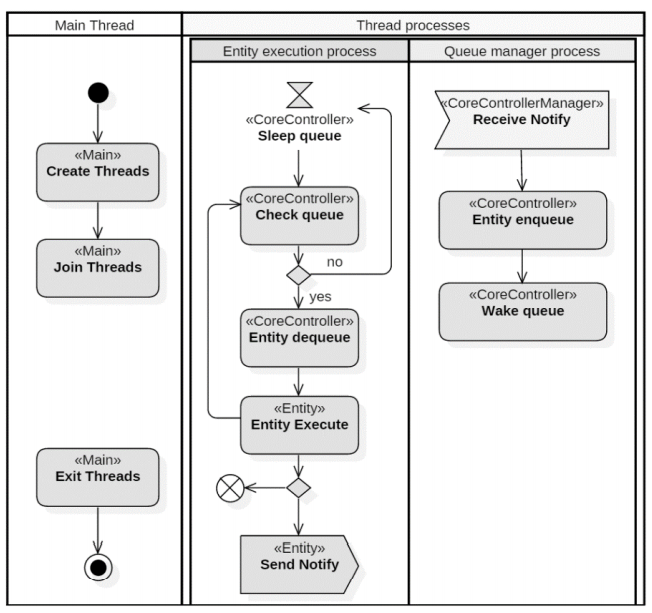
\includegraphics[width=.55\textwidth]{../figures/fw30_flow.png}
  \caption{Diagrama de atividades do controle de entidades do \textit{framework}
    C++ 3.0}
  \caption*{Fonte: \citeonline{schutz_2018}}
  \label{fig:fw3_flow}
\end{figure}

O processo de balanceamento da carga de trabalho do \textit{software} executado
pelo \textit{CoreControllerManager} é realizado de acordo com o método chamado
Motor de Balanceamento para Inferência Orientada a Notificações (\textit{Load
balancing engine for Notification-Oriented Inference - LobeNOI}), apresentado na
Figura \ref{fig:lobenoi}. Neste método primeiramente uma etapa de análise e
alocação dinâmica verifica o número de núcleos disponíveis do processador e
realiza a alocação inicial da aplicação, subsequentemente a etapa de análise e
alocação dinâmica monitora a utilização dos núcleos e realiza o balanceamento da
carga de trabalho em si por meio da realocação das entidades da aplicação
\cite{belmonte_2016}.

\begin{figure}[!htb]
  \centering
  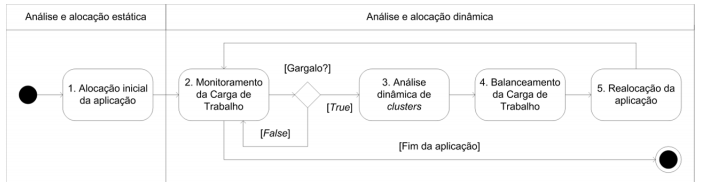
\includegraphics[width=\textwidth]{../figures/lobenoi.png}
  \caption{Visão geral do método \textit{LobeNOI}} \caption*{Fonte:
  \citeonline{belmonte_2016}}
  \label{fig:lobenoi}
\end{figure}

Ainda com base na implementação original do \textit{Framework} PON C++ 3.0 foi
implementado o NeuroPON em software paralelo \cite{schutz_2018}, o qual consiste
em uma nova arquitetura de treinamento e execução de Redes Neurais Artificias
(RNA) baseados em PON. O NeuroPON acrescenta algumas estruturas novas sobre o
\textit{Framework} PON C++ 3.0, de modo a permitir a sua construção sobre este
\textit{framework}.

A estrutura das entidades adicionadas pela NeuroPON é mostrada no diagrama da
Figura \ref{fig:neuro_struct}. Essas estruturas modelam os neurônios como
\textit{FBEs}, com \textit{Rules} e afins agregadas tratando de sua lógica dita
neural, bem como a classe de controle da rede neural em si como uma
\textit{NOPApplication} naturalmente com outras \textit{Rules} pertinentes.

\begin{figure}[!htb]
  \centering
  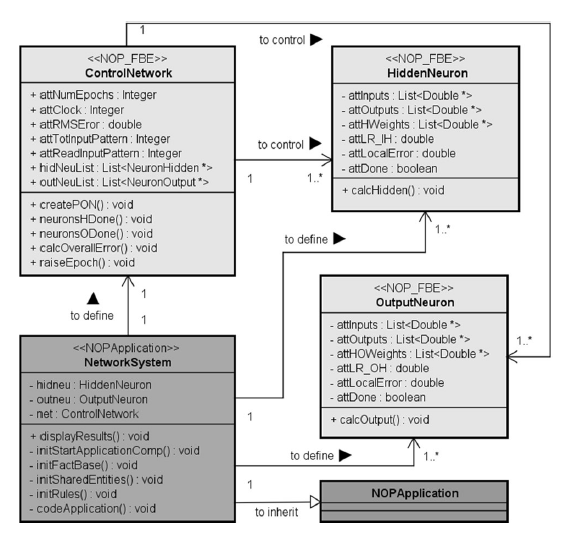
\includegraphics[width=.6\textwidth]{../figures/neuropon_struct.png}
  \caption{Estrutura do NeuroPON}
  \caption*{Fonte: \citeonline{schutz_2018}}
  \label{fig:neuro_struct}
\end{figure}

Conforme descrito acima, o \textit{Framework} PON C++ 3.0 possui mecanismos que
visam a organização e balanceamento da execução do programa de forma automática,
ou seja, sem a intervenção explícita do desenvolvedor, o qual alcançou bons.
Entretanto, o \textit{Framework} PON C++ 3.0 não alcançou os benefícios de
desempenho esperados pelo uso de paralelização em NeuroPON, tendo o tempo de
execução consideravelmente superior ao do \textit{Framework} PON C++ 3.0.

Tais problemas de desempenho se deram mais precisamente em uma aplicação
desenvolvida com a NeuroPON para o treinamento de uma RNA com
\textit{Multiplayer Perception} (MLP) utilizando o método de \textit{Back
Propagation} (BP) \cite{schutz_2018}. Os experimentos realizados com o
\textit{Framework} PON C++ 3.0 permitem observar a taxa de ocupação dos núcleos,
sendo mantido acima de 60\% em cada núcleo durante a execução da aplicação,
conforme mostrado na Figura \ref{fig:core_usage_cpp3}\footnote{Experimentos
realizados com um processador Core i7-3770 3.5 Ghz, 32 GB de memória RAM DDR3
1357MHz, com o sistema operacional Linux Ubuntu 16.04 LTS 64 bits.}. Entretanto,
isto não aportou um bom desempenho global em função das idiossincrasias da
arquitetura do NeuroPON, como a alta conectividade entre os seus constituintes,
não ser bem suportada pela abordagem do \textit{Framework} PON C++ 3.0 conforme
detalhado na tese de \citeonline{schutz_2018}.

No final das contas, no contexto dado, a execução de forma paralelizada trouxe
um aumento do tempo de execução do programa em PON. De forma geral, mecanismos
de controle de execução paralela (\textit{i.e.}, \textit{mutex},
\textit{threads}) causam um aumento do tempo de processamento. A utilização de
um número pequeno de neurônios nos experimentos faz com que as operações
paralelizadas sejam realizadas de forma muito rápida, fazendo com que a
aplicação gaste a maior parte do tempo nos mecanismos de controle, de modo que a
paralelização não traz melhoria nos tempos de execução \cite{schutz_2018}. Os
resultados, apresentados na Figura \ref{fig:pon_multi}, mostram que conforme
aumenta o número de núcleos utilizados, maior o tempo de execução
\cite{schutz_2018}.

\begin{figure}[!htb]
  \centering
  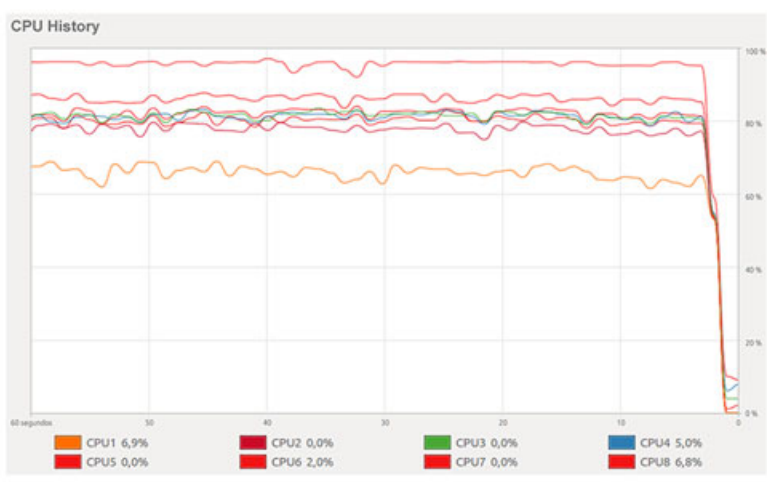
\includegraphics[width=.65\textwidth]{../figures/core_usage_cpp3.png}
  \caption{Taxa de utilização dos núcleos da CPU no treinamento de RNA MLP com método BP}
  \caption*{Fonte: \citeonline{schutz_2018}}
  \label{fig:core_usage_cpp3}
\end{figure}

Os resultados da NeuroPON paralela em \textit{Framework} PON C++ 3.0 poderiam
não depor contra o \textit{Framework} PON C++ 3.0 em si, mas contra a NeuroPON
finalmente. Entretanto, experimentos com a NeuroPON em outro \textit{framework}
demonstrariam que o problema enfim não seria nela, mas sim no Framework PON C++
3.0. Os resultados a NeuroPON neste outro \textit{framework} serão considerados
subsequentemente neste trabalho e se encontram na dissertação de mestrado de
\citeonline{negrini_2019}.

\begin{figure}[!htb]
  \centering
  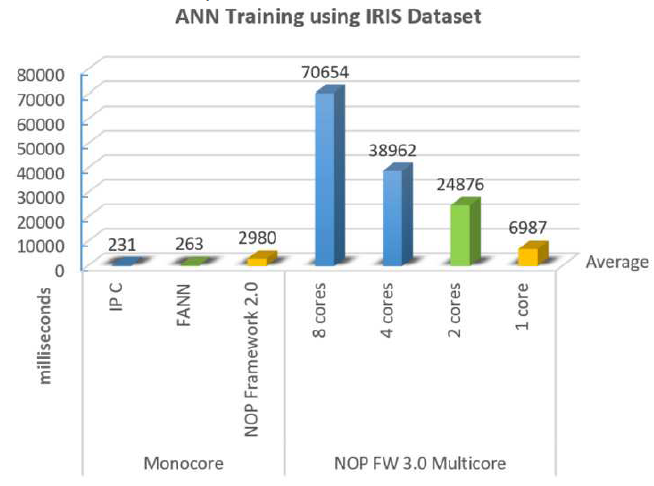
\includegraphics[width=.55\textwidth]{../figures/pon_multi_fix.png}
  \caption{Tempos de execução (em milissegundos) do treinamento de ANN MLP com método BP}
  \caption*{Fonte: \citeonline{schutz_2018}}
  \label{fig:pon_multi}
\end{figure}

\subsubsection{JuNOC++}

Todos os \textit{frameworks} em C++ apresentados até agora foram construídos
como evoluções com base nas versões anteriores. Além destes \textit{frameworks}
em C++, também há o JuNOC++ (\textit{Just a Notification Oriented} C++). Este
\textit{framework} se destaca por surgir não como uma evolução dos
\textit{frameworks} anteriores, mas sim como uma tentativa de
\citeonline{chierichi_2020} de criar um \textit{framework} do PON com base na
fundamentação apresentada na dissertação de \citeonline{msc_Banaszewski_2009}.
Desta forma, \citeonline{chierichi_2020} propõe uma estrutura que deixa de ser
mera reprodução dos \textit{frameworks} existentes, mas sim um novo
\textit{framework} independente com foco em programação em alto nível,
expressividade e desempenho.
%\footnote{A implementação do \textit{Framework}
%JuNOC++ está disponível em \url{https://github.com/GustavoChierici/JuNOCpp}}.

Do ponto de vista da estrutura do \textit{framework}, o JuNOC++ utiliza uma
estrutura baseada no pacote \textit{Core} do \textit{Framework} PON C++ 1.0,
incluindo melhorias principalmente observadas pela utilização de
\textit{templates} para a implementação de \textit{Attributes} e
\textit{Premises}. Esta estrutura de classes é ilustrada na Figura
\ref{fig:class_junoc}.

\begin{figure}[!htb]
  \centering
  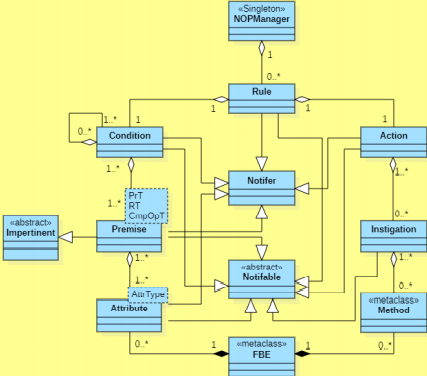
\includegraphics[width=.7\textwidth]{../figures/junoc_class.png}
  \caption{Diagrama de classes do JuNOC++}
  \caption*{Fonte: \citeonline{chierichi_2020}}
  \label{fig:class_junoc}
\end{figure}

O JuNOC++ utiliza recursos avançados, ditos modernos, da linguagem de
programação C++ e conceitos de programação genérica em seu desenvolvimento. Os
códigos \ref{cod:junoc_fbe} e \ref{cod:junoc_cpp} apresentam, respectivamente,
um \textit{FBE} e sua respectiva implementação com o JuNOC++. No código em C++
com o JuNOC++ podem ser observadas as melhorias alcançadas no sentido de
facilitar a programação em alto nível. Com o uso extensivo de \textit{macros} e
sobrecarga de operadores a construção das entidades do PON, como a \textit{Rule}
\textit{rlChange} em destaque neste código, pode ser feita de maneira muito
similar à sua construção em \textit{LingPON} e natural ao PON.

\noindent
\begin{minipage}{.45\textwidth}
  \begin{lstlisting}[caption = {\textit{FBE} para exemplo no JuNOC++},
    source = {\citeonline{chierichi_2020}},
    label = {cod:junoc_fbe}]
fbe Main
{
  private boolean atStatus = false
  private boolean atStatus = false

  private method mtChange()
  {
    this.atStatus=true
  }
  rulerlChange this.atStatus == true
          or this.atStatus2 == true
  {
    call{this.mtChange()}
  }
  main
  {
    this.atStatus=true
    this.atStatus2=true
  }
}
    \end{lstlisting}
\end{minipage}\hfill
\begin{minipage}{.45\textwidth}
  \begin{lstlisting}[caption = {Código em C++ para exemplo no JuNOC++},
    source = {\citeonline{chierichi_2020}},
    label = {cod:junoc_cpp}]
class Main
{
 private:
  NOP::Attribute<bool> atStatus;
  NOP::Attribute<bool> atStatus2;
  NOP::Rule rlChange;
 public:
  Main();
 private:
  voidmtChange();
};

Main::Main():
  atStatus{false, "atStatus"},
  atStatus2{false, "atStatus2"},
  rlChange{"rlChange"}
{
  RULE(rlChange, atStatus == true
      or atStatus2 == true)
    INSTIGATE([&](){mtChange();})
  ENDRULE

  atStatus = true;
  atStatus2 = true;
}

voidMain::mtChange()
{
  atStatus=true;
}

  \end{lstlisting}
\end{minipage}

Em experimentos reslizados, o JuNOC++ inclusive demostrou desempenho superior
aos outros \textit{frameworks} em linguagem de programação C++ considerados,
nomeadamente os \textit{Frameworks} PON C++ 2.0 e 4.0\footnote{Neste experimento
também foi considerada uma implementação em \textit{namespaces}, que é um alvo
de compilação da LingPON, apresentado neste trabalho na Seção
\ref{sec:lingpon}}. Destaca-se apenas que a versão do \textit{Framework} PON C++
4.0 neste experimento era uma versão prototipal, que não reflete o desempenho
real da sua versão final, que apresenta desempenho superior ao
\textit{Framework} PON C++ 2.0, conforme será apresentado no Capítulo
\ref{ch:result}.

\begin{figure}[!htb]
  \centering
  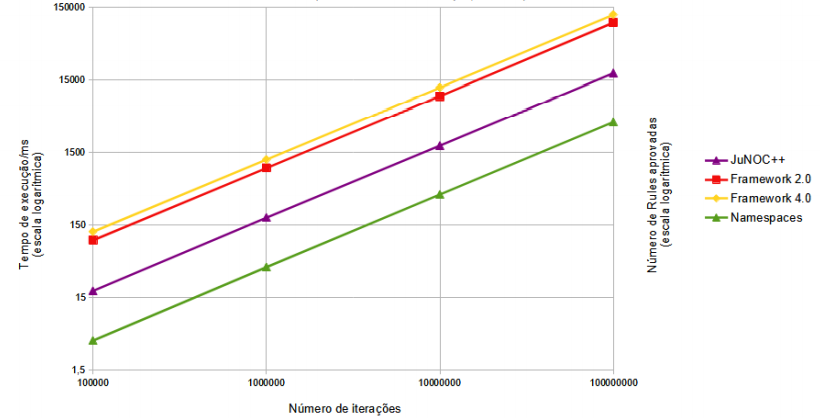
\includegraphics[width=.85\textwidth]{../figures/junoc_graph.png}
  \caption{Gráfico dos restultados de experimento com o JuNOC++}
  \caption*{Fonte: \citeonline{chierichi_2020}}
  \label{fig:exp_junoc}
\end{figure}

O \textit{Framework} PON C++ 4.0 em JuNOC++ foram desenvolvidos em paralelo,
assim sendo, muitas das melhorias propostas são consideradas em ambos. O JuNOC++
aproveitou principalmente as implementações com \textit{templates} introduzidas
pelo \textit{Framework} PON C++, enquanto este buscou inspiração nas melhorias
introduzidas pelo JuNOC++ para facilitar a programação em alto-nível. Ainda
assim, ambos os \textit{frameworks} possuem propostas diferentes, sendo que o
\textit{Framework} PON C++ 4.0 se preocupa em disponibilizar uma materialização
mais estável, com desenvolvimento orientado a testes, incorporando conceitos de
paralelismo, o JuNOC++ é ainda uma materialização de cunho prototipal,
explorando a flexibilização da construção das entidades, com foco na programação
em alto nível.

\subsubsection{Implementações realizadas com o \textit{Framework} PON C++
  2.0}\label{sec:ex_fw2}

Inicialmente, de modo a possibilitar levantar as deficiências do
\textit{Framework} PON C++ 2.0, apontadas na Seção \ref{sec:problemas}, e servir
também como conhecimento de base para a implementação de um novo
\textit{framework}, foram desenvolvidas aplicações utilizando o
\textit{Framework} PON C++ 2.0. Com o desenvolvimento destas aplicações era
objetivado ganhar experiência no desenvolvimento em aplicações com o PON, em
particular com o \textit{Framework} PON C++ 2.0, de forma a facilitar o
entendimento dos pontos de melhoria a serem implementados. Essas implementações
são descritas com maiores detalhes nas seções seguintes.

\paragraph{Futebol de Robôs}

A primeira aplicação desenvolvida pelo autor deste trabalho utilizando o PON foi
no âmbito de Futebol de Robôs. Esta aplicação foi desenvolvida no contexto da
disciplina de Tópicos Especiais em Engenharia da Computação: Paradigma Orientado
a Notificações, via PPGCA, na UTFPR, durante o terceiro trimestre de 2019
\cite{lima_2020}. Tal implementação inspirou-se em trabalho prévio desenvolvido
por \citeonline{msc_santos_2017}, ainda que esta nova implementação tenha sido a
partir de uma versão mais prototipal do trabalho dele por ser a que se encontrou
disponível. Em tempo, o trabalho foi conjunto entre cinco discentes da
disciplina, sendo que cada qual montou um dado conjunto de \textit{Rules}
subsequentemente integradas \cite{lima_2020}.

Neste âmbito, de forma a aplicar os conhecimentos adquiridos durante a
disciplina foi proposto o desenvolvimento de uma aplicação de controle de robôs
em \textit{Framework} PON C++ 2.0, em contexto de Futebol de Robôs, para
execução em ambiente de simulação. Essa aplicação consiste do controle de duas
equipes, compostas cinco robôs cada, executada em um ambiente virtual que simula
um campo de futebol. Uma tela da execução deste ambiente de simulação é mostrada
na Figura \ref{fig:futebol_robos}, na qual é possível observar o campo e os
robôs de ambos os times.

Nesse cenário, a parte da aplicação desenvolvida em \textit{Framework} PON C++
2.0 é responsável por receber e processar comandos de um juiz virtual que envia
os comados da partida (\textit{e.g.}, início, parada, falta etc.), assim como a
aplicação desenvolvida em \textit{Framework} PON C++ 2.0 é responsável por
controlar de forma autônoma todos os robôs de ambas as equipes. Cada equipe é
controlada por uma instância independente da aplicação em PON \cite{lima_2020}.
Para o desenvolvimento em PON desta aplicação foi utilizado o \textit{Framework}
PON C++ 2.0 conforme o que definido em \citeonline{msc_Ronszcka_2012} e
\citeonline{msc_valenca_2012}. 

\begin{figure}[!htb]
  \centering
  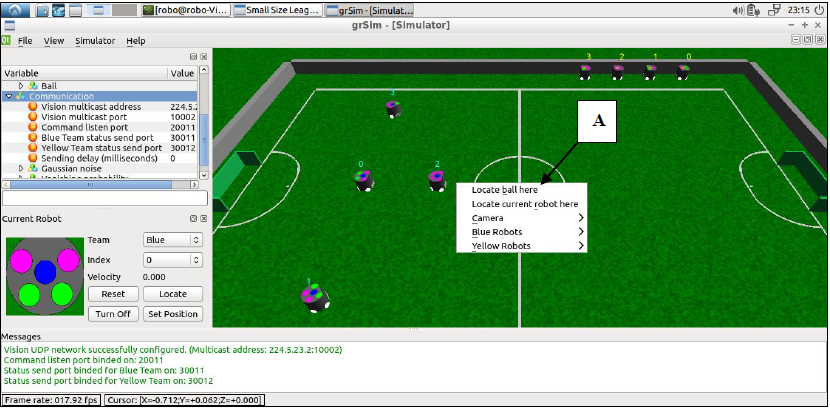
\includegraphics[width=0.95\textwidth]{../figures/futebol_robos.png}
  \smallskip
  \caption{Tela principal do ambiente de simulação do futebol de robôs}
  \caption*{Fonte: \citeonline{lima_2020}}
  \label{fig:futebol_robos}
\end{figure}

No escopo deste trabalho foi utilizado um ambiente previamente configurado e
funcional, contendo um conjunto básico de \textit{Rules} e \textit{FBEs} já
existentes, fruto de uma versão prototipal dos esforços da dissertação de
mestrado de \citeonline{msc_santos_2017}, conforme já especificado acima.
Baseado nessa estrutura inicial, representada pelo diagrama de classes da Figura
\ref{fig:class_futebol}, foram apenas desenvolvidas novas \textit{Rules},
utilizando os \textit{FBEs} já existentes \textit{RobotPON} e
\textit{StrategyPON}. O artigo-relatório contendo todo o desenvolvimento deste
projeto é apresentado na íntegra no \nameref{ch:apendice_futebol}, para fins de
registro na dissertação.

\begin{figure}[!htb]
    \centering
    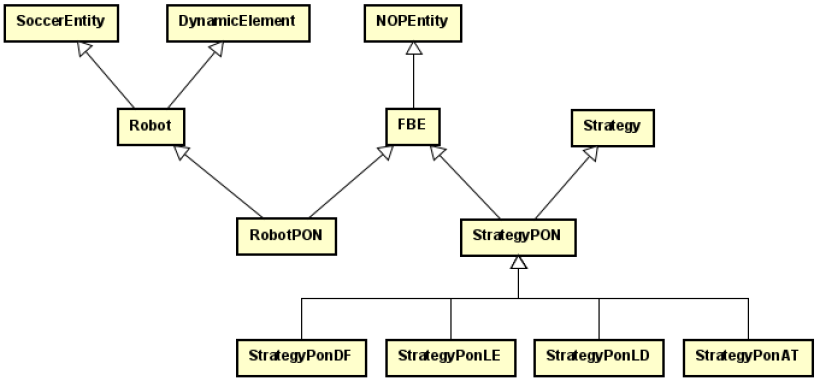
\includegraphics[width=0.7\textwidth]{../figures/class_futebol.png}
    \smallskip
    \caption{Diagrama de classes do futebol de robôs}
    \caption*{Fonte: \citeonline{lima_2020}}
    \label{fig:class_futebol}
\end{figure}

\FloatBarrier

Durante o desenvolvimento do trabalho foram encontradas algumas dificuldades,
principalmente no que se refere ao uso do ambiente de desenvolvimento proposto.
Isto primeiramente pelo fato do mesmo ser disponibilizado inicialmente na forma
de uma máquina virtual que necessitava se configurada e instalada. Ainda, uma vez
instalada a máquina e o ambiente como um todo, percebeu-se que não continha
todas as \textit{Rules} e, principalmente, não continha \textit{FBEs} com seus
\textit{Methods} e \textit{Attributes} de acordo com a dissertação de
\citeonline{msc_santos_2017}, concluindo-se subsequentemente que se tratava de
um código mais prévio ou prototipal \cite{lima_2020}.

No contexto acima relatado, especialmente devido ao ambiente conter um número de
\textit{FBEs} implementados muito pequeno, não havia recursos para se fazer a
criação das novas \textit{Rules} de forma muito abundante. Ainda, perceberam-se
outros fatores em algo obstantes, como o fato de recursos mais avançados do
\textit{framework}, como \textit{Master Rule} e \textit{SubConditions}, não
possuírem uma construção tão intuitiva quanto seria possível, bem como não haver
instruções de utilização adequadas, o que dificultou a implementação das
\textit{Rules} que foram criadas.

Em função destas dificuldades postas, também percebeu-se a curva não tão suave
(conforme habilidade de cada qual) de aprendizado do \textit{Framework} PON C++
2.0, ao menos neste exemplo em questão. Não obstante as dificuldades, a criação
de conjuntos de \textit{Rules} pelos discentes permitiu bem compreender o PON.
Ademais, também foi possível observar propriedades do PON, como os conjuntos de
\textit{Rules} trabalhando harmonicamente no final da implementação, isto sem
esforços extraordinários de integração em função do nível de desacoplamento
entre eles.

\paragraph{Jogo NOPUnreal}\label{sec:nopunreal}

A segunda aplicação, já desenvolvida após certa familiarização com o
desenvolvimento em PON foi realizada sob a forma de um jogo. A proposta desta
aplicação era realizar a integração do \textit{Framework} PON C++ 2.0 com uma
API complexa de desenvolvimento de jogos. Para este fim foi escolhida a Unreal
Engine. Em tempo, este foi um trabalho desenvolvido no contexto da disciplina de
Estudo Especial — Paradigmas de Programação, via CPGEI, na UTFPR, durante o
primeiro trimestre de 2020 \cite{neves_2020}\footnote{Este trabalho também foi
apresentado sob a forma de minicurso no SICITE 2020}. A estrutura básica do jogo
consiste em uma nave controlada pelo jogador com o objetivo de neutralizar todos
os inimigos. A Figura \ref{fig:jogo_fw2} mostra uma tela do jogo desenvolvido,
na qual o jogador é representado pela nave cinza, e os inimigos pelas naves
amarelas.

\begin{figure}[!htb]
  \centering
  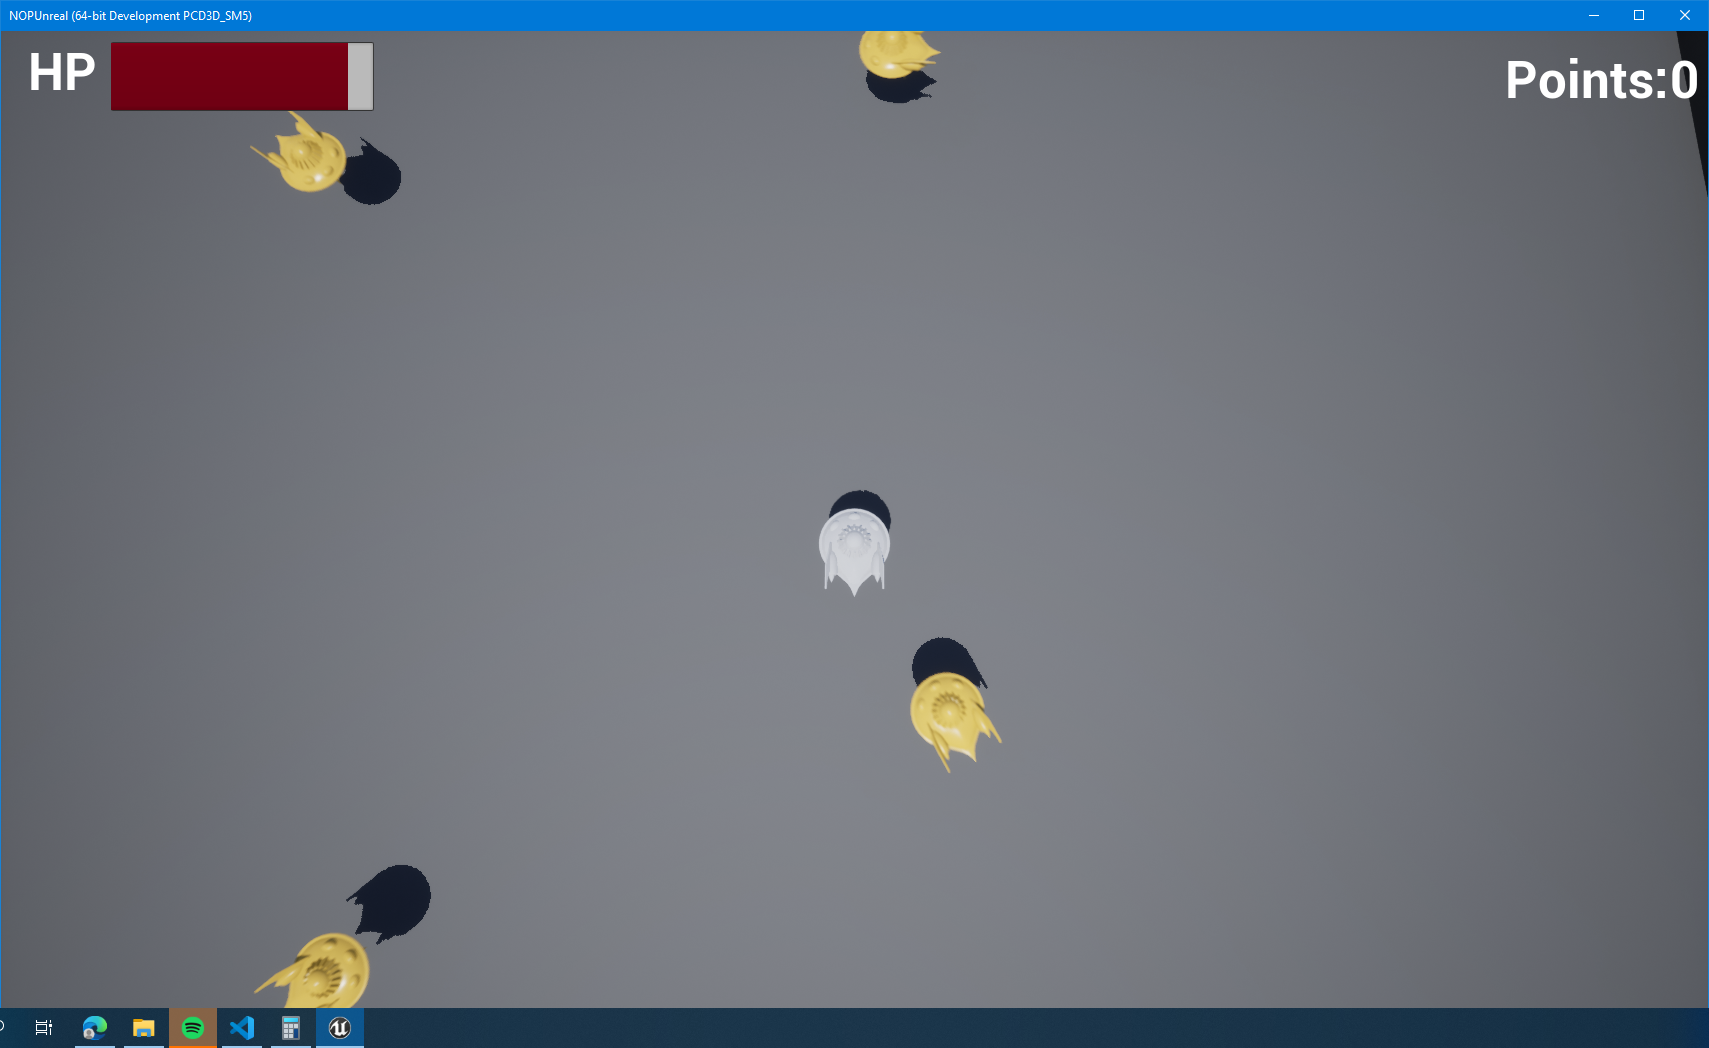
\includegraphics[width=\textwidth]{../figures/game.png}
  \smallskip
  \caption{\textit{Screenshot} do jogo desenvolvido} \caption*{Fonte:
      \citeonline{neves_2020}}
  \label{fig:jogo_fw2}
\end{figure}

A Unreal Engine foi escolhida por ser o motor gráfico mais utilizado no
desenvolvimento de jogos e aplicações gráficas comerciais, chegando a ser
utilizada em cerca de 20\% dos jogos de computador \cite{neves_2020}. O
desenvolvimento desta aplicação foi realizado utilizando tanto com o POO como o
PON, de modo a permitir a comparação da facilidade de programação utilizando os
dois paradigmas. De modo geral o desenvolvimento foi mais fácil e rápido
utilizando o PON, chegando a obter um tempo de desenvolvimento até 38.62\%
menor, porém a verbosidade do \textit{Framework} PON C++ 2.0 resultou em um
código-fonte com 12.16\% mais linhas que a implementação equivalente no POO
\cite{neves_2020}.

Um dos elementos que dificulta a aplicação do PON neste projeto é a rigidez da
estrutura da API da Unreal Engine, sendo implementada utilizando o POO e fazendo
uso extensivo de lógica sequencial na sua execução. Neste contexto, o
desenvolvedor é obrigado a utilizar as estruturas e classes próprias da Unreal
Engine para a sua implementação. Na Figura \ref{fig:class_jogo_fw2}\footnote{Nos
diagramas de classe construídos com a ferramenta PlantUML o símbolo C em um
círculo verde identifica classes concretas, já o símbolo A sobre um círculo azul
identifica classes abstratas} é mostrado o diagrama de classes do jogo
desenvolvido, no qual é importante destacar que as classes implementadas em PON,
derivadas da classe \textit{FBE}, também são derivadas das classes próprias de
Unreal Engine (\textit{APawn}, \textit{AActor}, \textit{UObject},
\textit{UActorComponent} e \textit{AInfo}). Deste modo pode ser dito que o
código implementado é, na verdade, multiparadigma, pois utiliza tanto o PON como
o POO na sua implementação. 

Nesse contexto de programação multiparadigma, o PON
é utilizado para implementar a lógica referente ao comportamento dos inimigos e
às regras do jogo, enquanto o POO é utilizado para a implementação dos elementos
gráficos da aplicação. O artigo-relatório contendo o desenvolvimento deste
projeto, inclusive contendo a especificação completa de todas as \textit{Rules}
implementadas, é apresentado na íntegra no \nameref{ch:apendice_nopunreal}.

A implementação deste projeto realçou algumas das deficiências ou imperfeições
do \textit{Framework} PON C++ 2.0. Um dos principais problemas foi a baixa
flexibilidade de tipos, que fica bem evidente devido à Unreal Engine utilizar
muitos tipos próprios, como estruturas, enumerações e classes (\textit{e.g.}
\textit{FVector}, \textit{FString} etc.).

\begin{figure}[!htb]
  \centering
  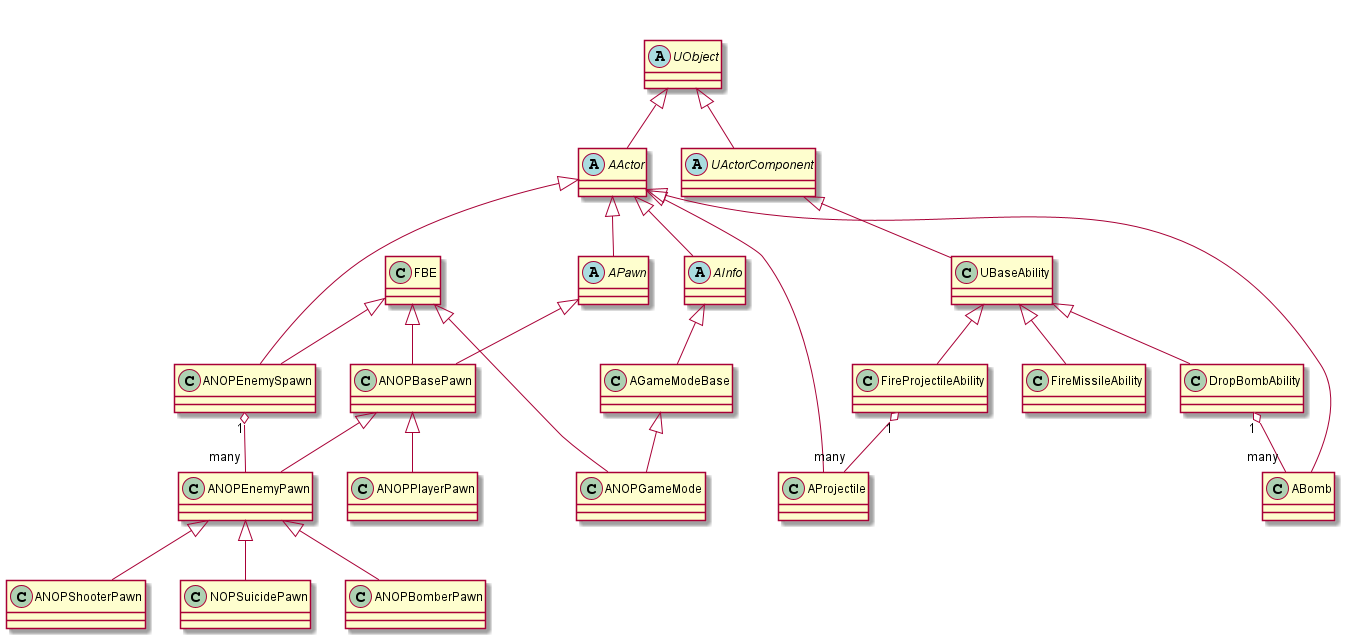
\includegraphics[width=\textwidth]{../out/diagrams/class_diagram_nop/NOPUnreal.png}
  \smallskip
  \caption{Diagrama de classes do jogo desenvolvido}
  \caption*{Fonte: \citeonline{neves_2020}}
  \label{fig:class_jogo_fw2}
\end{figure}

O fato do \textit{Framework} PON C++ 2.0 somente permitir o uso de seus tipos
pré-definidos (\textit{int}, \textit{double}, \textit{bool} e \textit{string})
faz com que seja necessário converter os tipos próprios da Unreal Engine para a
utilização em conjunto com as entidades do PON. Alguns exemplos que melhor
ilustram esse problema são apresentados abaixo. No Código
\ref{cod:integer_cast}, um \textit{Attribute} do tipo \textit{int} é utilizado
para implementar um tipo que utiliza uma enumeração, exigindo que seja realizada
uma conversão de tipos.

\begin{lstlisting}[caption = {Uso de \textit{static\_cast} para converter enumerações}, float=htb,
source = {Autoria própria},
label = {cod:integer_cast}]
INTEGER(this, atStrategym static_cast<int>(ENOPEnemyStrategy:EFollow));
\end{lstlisting}

Por sua vez, também o Código \ref{cod:fvector} mostra a estrutura FVector, muito
utilizada em todo o código para representar a posição no espaço tridimensional
dos objetos. Porém, o uso dela em \textit{Premises} e \textit{Attributes} é
impossível, pois não é um tipo básico suportado. Assim, faz necessários
desmembramentos e afins para seu uso. 

\begin{lstlisting}[caption = {Estrutura \textit{FVector} da Unreal Engine}, float=htb,
source = {Autoria própria},
label = {cod:fvector}]
struct FVector {
    float X;
    float Y;
    float Z;
}
\end{lstlisting}

Por fim, o Código \ref{cod:flexibilidade_pon} apresenta uma situação na qual é
necessário criar \textit{Premises} muito semelhantes, porém, com avaliações
opostas. Devido à baixa flexibilidade algorítmica não permitir a criação de
\textit{Conditions} com composição de \textit{Premises} utilizando declaração de
operações lógicas mais diversas sobre elas, como seria o caso de uma operação de
negação, ocorre este tipo de redundância estrutural.

\begin{lstlisting}[caption = {Uso de premissas redundantes no PON}, float=htb,
source = {Autoria própria},
label = {cod:flexibilidade_pon}]
PREMISE(prIsFarFromTarget, atDistanceToTarget, 800.0f, Premise::GREATEROREQUAL, Premise::STANDARD, false);
PREMISE(prIsNOTFarFromTarget, atDistanceToTarget, 800.0f, Premise::SMALLERTHAN, Premise::STANDARD, false);
\end{lstlisting}

Em suma, o desenvolvimento de ambas estas aplicações permitiu principalmente
observar as limitações do \textit{Framework} PON C++ 2.0, explorados em detalhes
na Seção \ref{sec:problemas}. Ainda, essas experiências serviram também como
fator motivador para a proposta do \textit{Framework} PON C++ 4.0.

\subsubsection{Considerações sobre os \textit{frameworks} do PON em C++}

De forma geral, as materializações do PON por meio de \textit{frameworks} em
linguagem de programação C++ representam uma grande contribuição ao estado da
técnica do PON, possibilitando o desenvolvimento de aplicações que permitiram
avaliar e comparar o desempenho do PON
\cite{msc_Banaszewski_2009,msc_Ronszcka_2012,msc_valenca_2012}. Nas
materializações de \textit{frameworks} em C++, foram desenvolvidas a maior parte
das aplicações feitas em PON conforme
\cite{msc_Ronszcka_2012,msc_santos_2017,doc_ronszcka_2019}.

Houve também o desenvolvimento de diversas aplicações como os
\textit{frameworks} do PON em C++, nomeadamente a aplicação Mira ao Alvo
\cite{msc_Banaszewski_2009,msc_Ronszcka_2012,msc_valenca_2012}, o Futebol de
Robôs \cite{msc_santos_2017,lima_2020}, o jogo NOPUnreal \cite{neves_2020} e
também o NeuroPON \cite{belmonte_2012,belmonte_2016,doc_Schutz_2019}. Todas
estas aplicações desenvolvidas são interessantes em pertinentes, demonstrando
diversos casos de uso do PON, assim como servindo de \textit{benchmarks}, como o
caso da aplicação Mira ao Alvo (que posteriormente evoluí sob nova forma de rede
de sensores), frequentemente utilizada para comparações de desempenho entre os
\textit{frameworks}. 

Apesar disso, essas aplicações têm utilização limitada ao contexto do grupo de
pesquisa do PON, de forma que estes \textit{frameworks} carecem de
\textit{benchmarks} universalizados, mais conhecidos pela comunidade científica.
Salienta-se inclusive que aplicações como o Futebol de Robôs não são
particularmente adequadas para fins \textit{benchmark} em si, por ser uma
aplicação que não se interessa em tempos de execução.

\subsection{\textit{Frameworks} PON Java/C\# 1.0}\label{sec:csharp_java}

Não obstante, além das materializações em C++, também houve a materialização na
forma de \textit{framework} nas linguagens Java e C\#, ainda que assaz
prototipais ou ao menos ainda não utilizadas largamente. Esta seção trata de
forma unificada destas duas materializações em linguagens diferentes, pois as
mesmas são materializações equivalentes principalmente ao \textit{Framework} PON
C++ 1.0 e sob a forma de adaptações dele para tais linguagens
\cite{henzen_2015}.

O objetivo destas materializações foi adaptar o \textit{Framework} PON C++ 1.0
para Java e C\# utilizando técnicas de programação semelhantes, que padronizam e
facilitam a manutenção do código. Estas materializações se justificam pelo
grande número de programadores que utilizam as linguagens Java e C\#, sendo
muito utilizadas, principalmente, em aplicações móveis e web \cite{henzen_2015}.
A linguagem Java também é adotada como principal linguagem no ensino de
programação em diversas universidades, o que contribui para o grande número de
programadores utilizando a mesma \cite{henzen_2015}.

 Para a comparação dos resultados entre as materializações de C++, Java e C\#
foi desenvolvida uma aplicação para controle de um portão eletrônico. A
implementação desta aplicação consiste na criação de duas \textit{Rules}, uma
para abrir e outra para fechar o portão, com base nos \textit{FBEs} do portão,
que encapsula o estado do portão (aberto ou fechado), e controle remoto, que
encapsula o estado do botão (pressionado ou não) \cite{henzen_2015}. As
particularidades das implementações em cada uma das linguagens são apresentadas
nas seções seguintes.


\subsubsection{\textit{Framework} PON Java 1.0}\label{sec:java}

Algumas alterações foram necessárias para implementar o \textit{framework} em
Java, como o fato de a linguagem Java não possuir o conceito herança múltipla,
para isto sendo utilizado como alternativa o conceito de \textit{Interface}. Um
trecho da aplicação desenvolvida com o \textit{Framework} PON Java 1.0 é
apresentado no Código \ref{cod:java_nop}.

\begin{lstlisting}[caption = {Exemplo de \textit{Rule} do portão eletrônico em Java},
source = {Adaptado de \citeonline{henzen_2015}},
label = {cod:java_nop}]

Condition cond1R01 = new Condition(Condition.CONJUNCTION);
cond1R01.addPremise(new Premise(remoteControl.atRemoteControlStatus, NBoolean.TRUE_NOP, Premise.EQUAL, false));
SubCondition subcond1R01 = new SubCondition(SubCondition.DISJUNCTION, false);
subcond1R01.addPremise(new Premise(gate.atGateStatus, 0, Premise.EQUAL, false));
subcond1R01.addPremise(new Premise(gate.atGateStatus, 5, Premise.EQUAL, false));
cond1R01.addSubCondition(subcond1R01);

Action actR01 = new Action();
actR01.addInstigation(new Instigation(gate.mtOpening));
actR01.addInstigation(instStatusOff);

Rule rule1 = new Rule("Opening gate", scheduler, cond1R01, actR01, false);
\end{lstlisting}

\subsubsection{\textit{Framework} PON C\# 1.0}\label{sec:csharp}

Por sua vez, na implementação de \textit{framework} com a linguagem C\# foi
utilizado conceito de \textit{Delegate} no lugar de ponteiros para funções
\cite{henzen_2015}. Um trecho da aplicação desenvolvida com o \textit{Framework}
PON C\# 1.0 é apresentado no Código \ref{cod:csharp}.

\begin{lstlisting}[caption = {Exemplo de \textit{Rule} do portão eletrônico em C\#},
source = {Adaptado de \citeonline{henzen_2015}},
label = {cod:csharp}]
Condition cond1 = new Condition(Condition.CONJUNCTION);
cond1.addPremise(new Premise(remoteControl.bIsPressed,NBoolean.TRUE_NOP,Premise.EQUAL,false));
cond1.addPremise(new Premise(gate.GateStatus,true,Premise.EQUAL,false));

Action action1 = new Action();
action1.addInstigation(new Instigation(remoteControl.bIsPressed,false));
action1.addInstigation(new Instigation(gate.mtOpenGate));

Rule rule1 = new Rule("Open gate", scheduler, cond1, action1, false);
\end{lstlisting}

\subsubsection{Comparações}

Foram realizados testes com 10.000, 100.000, 20.0000 e 500.000 iterações de
fechamento do portão\footnote{Para este teste foi utilizado um computador modelo
Apple Macbook Pro, Core i5 2.5 Ghz, 6 GB de memória RAM, com o sistema
operacional Windows 10 Preview.}, com os resultados mostrados na Figura
\ref{fig:comp_henzen}. O desempenho dos \textit{frameworks} em Java e C\# foi
satisfatório, inclusive superando o desempenho do \textit{Framework} PON C++ 1.0
neste cenário, sendo o \textit{framework} Java aquele que apresentou o melhor
desempenho. Entretanto, seriam necessários mais experimentos para avaliar como
ficariam esses desempenhos, inclusive em relação ao \textit{Framework} PON C++
2.0.

\begin{figure}[!htb]
  \centering
  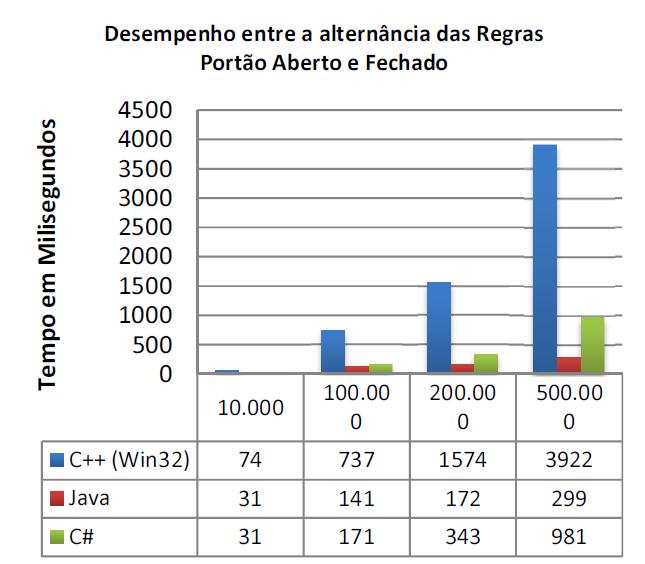
\includegraphics[width=.5\textwidth]{../figures/comp_henzen.png}
  \caption{Comparação de desempenho das aplicações em C++, Java e C\#}
  \caption*{Fonte: \citeonline{henzen_2015}}
  \label{fig:comp_henzen}
\end{figure}

Isto dito, o desenvolvimento destes \textit{frameworks} demonstrou ser possível
a implementação de um \textit{framework} do PON em Java e C\#, inspirado no
\textit{Framework} PON C++ 1.0, sem haver descaracterização das técnicas
empregadas na implementação original \cite{henzen_2015}. Apesar do aspecto
prototipal destes \textit{frameworks}, seu desenvolvimento abriu novos caminhos
de pesquisa para o PON explorando tais plataformas, como o subsequente
desenvolvimento do \textit{Framework} PON C\# IoT.

\FloatBarrier

\subsection{\textit{Framework} PON C\# IoT}

Na materialização \textit{Framework} PON C\# IoT, desenvolvida à luz dos
esforços de \citeonline{msc_oliveira_2019} introduzem uma versão com o foco em
Internet das Coisas (IoT - \textit{Internet of Things}). Do ponto de vista de
implementação esta versão se inspira no \textit{framework} PON C++ 2.0 e
adapta/evolui o \textit{Framework} PON C\# 1.0, com o seu diferencial sendo a
proposta da distribuição em rede das entidades do PON, permitindo a aplicação
dos conceitos de IoT, por meio de paralelismo, distribuição e a capacidade de
reconfiguração das \textit{Rules} em tempo de execução \cite{msc_oliveira_2019}.

A Figura \ref{fig:classes_pon_iot} apresenta o diagrama de classes do
\textit{Framework} PON C\# IoT. Apesar de apresentar uma estrutura bastante
similar ao \textit{Framework} PON C++ 2.0 e C\# 1.0 também é possível observar
neste diagrama a adição de classes específicas para aplicação no ambiente
distribuído, como a classes \textit{SensorFBE} e \textit{NotificationNetwork}.

\begin{figure}[!htb]
  \centering
  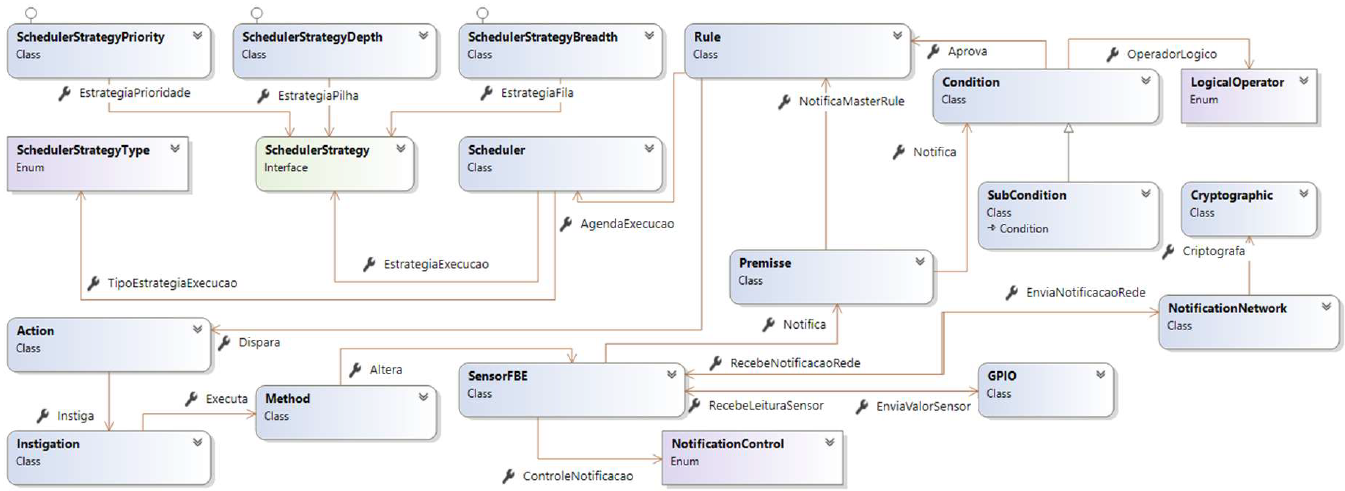
\includegraphics[width=\textwidth]{../figures/classes_pon_iot.png}
  \caption{Diagrama simplificado de classes do \textit{Framework} PON C\# IoT}
  \caption*{Fonte: \citeonline{msc_oliveira_2019}}
  \label{fig:classes_pon_iot}
\end{figure}

Este \textit{Framework} PON C\# IoT utiliza uma unificação das entidades
\textit{FBE} e \textit{Attribute}, chamada de \textit{SensorFBE}, na qual o
\textit{FBE} possui apenas um único \textit{Attribute}, relativo a leituras do
sensor ou atuador. O \textit{SensorFBE} também possui alguns outros atributos
não relativos ao mecanismo de notificações do PON, como identificador único,
nome, tipo, intervalo de leitura, e outras definições relativas ao
sensor/atuador\footnote{Este \textit{framework} foi projetado para trabalhar com
uma placa RaspberryPi, portanto apresenta configurações específicas para lidar
diretamente com as entradas e saídas desta placa} \cite{msc_oliveira_2019}. A
entidade \textit{SensorFBE} ainda possui outras variáveis que controlam a forma
de notificação das \textit{Premises}, como o controle de notificação, podendo
ser \textit{Always}, \textit{On change} ou \textit{Never}. As entidades
\textit{SensorFBE} podem ser executadas de forma distribuída, sendo capazes de
notificarem \textit{Premises} sendo executadas em outros dispositivos remotos.

O processo de notificação é executado de forma paralela, utilizando a função
\textit{Parallel.ForEach} do C\#, de modo que cada notificação gerada pelo
\textit{SensorFBE} é processada em uma \textit{thread} diferente
\cite{msc_oliveira_2019}. Ainda, nas situações nas quais a entidade a ser
notificada pode estar em um ambiente remoto, como em outro dispositivo, a
notificação é enviada utilizando o mecanismo que permite o envio para outros
clientes, o \textit{IoT.NotificationClient.Notification}, com o uso do método
\textit{Send}. Deste modo a notificação é enviada para os outros dispositivos
via protocolo TCP/IP \cite{msc_oliveira_2019}. A Figura \ref{fig:ativ_pon_iot}
ilustra as atividades executadas durante o processo de leitura de um sensor
físico utilizando o \textit{Framework} PON C\# IoT.

\begin{figure}[!htb]
  \centering
  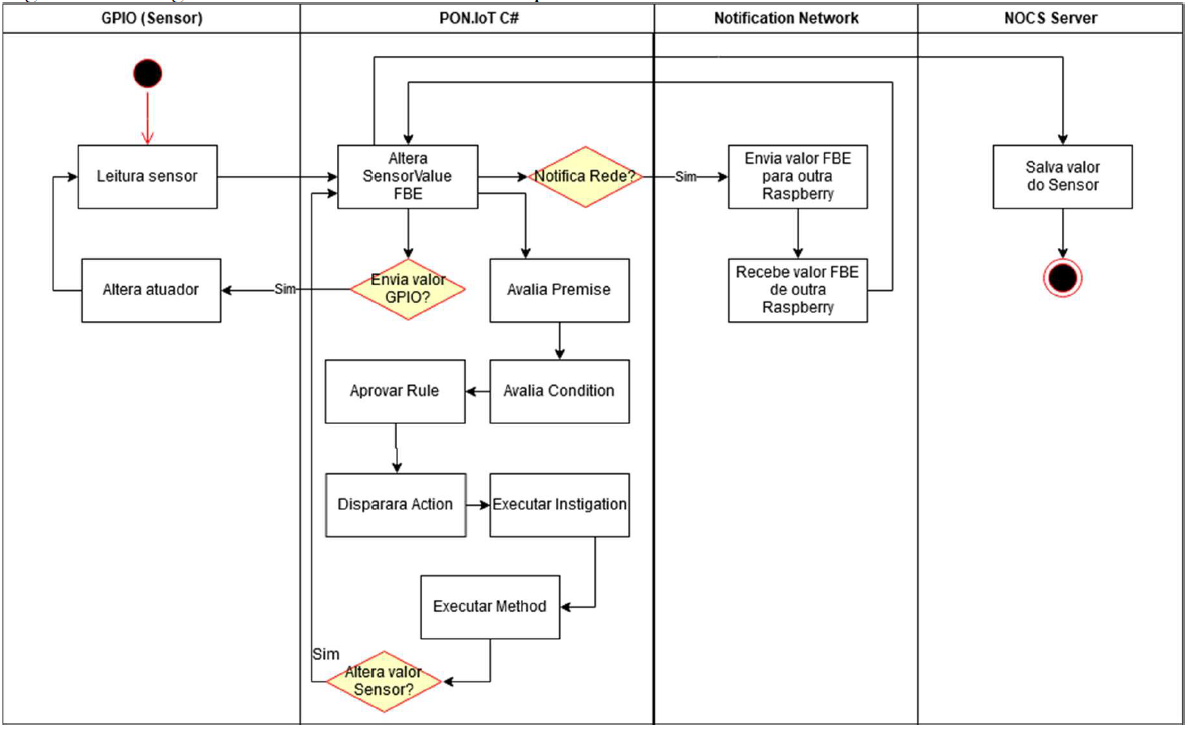
\includegraphics[width=0.9\textwidth]{../figures/pon_iot_flow.png}
  \caption{Diagrama de atividades do PON C\# IoT}
  \caption*{Fonte: \citeonline{msc_oliveira_2019}}
  \label{fig:ativ_pon_iot}
\end{figure}

O \textit{Framework} PON C\# IoT também faz o uso do conceito de impertinência
dinâmica de \textit{Attributes} e \textit{Premises}. Neste mecanismo, sem a
interferência do desenvolvedor, a própria \textit{Condition} define a
impertinência de suas \textit{Premises}, baseado no valor lógico das outras
\textit{Premises} e estas de seus respectivos \textit{Attibutes}, baseado na
relevância de cada \textit{Premise} na aprovação da \textit{Condition}. Por
exemplo, no caso de uma \textit{Condition} com operação lógica de conjunção, as
demais \textit{Premises} somente tem suas notificações ativadas após a primeira
\textit{Premise} definida como mais relevante possuir valor lógico verdadeiro
\cite{msc_oliveira_2019}. 

Esse \textit{framework} foi aplicado para o desenvolvimento do NOCS
(\textit{Notification Oriented Care System}), com a utilização do ambiente
distribuído mostrado na Figura \ref{fig:pon_iot}, por meio da conexão dos
sensores e atuadores utilizando a entidade \textit{SensorFBE} em um dispositivo
RaspberryPi remoto (NOCS Control), que se comunica com um servidor central (NOCS
Server), capaz de executar os processos de interface com o usuário e comunicação
com outros dispositivos \cite{msc_oliveira_2019}. 

\begin{figure}[!htb]
  \centering
  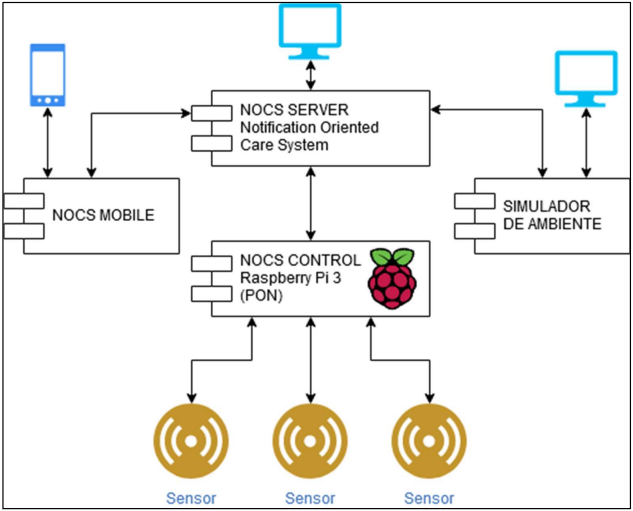
\includegraphics[width=.55\textwidth]{../figures/pon_iot.png}
  \caption{Diagrama de componentes PON C\# IoT}
  \caption*{Fonte: \citeonline{msc_oliveira_2019}}
  \label{fig:pon_iot}
\end{figure}

Ainda, o NOCS Server disponibiliza uma interface web na qual os usuários podem
visualizar os estados dos sensores/atuadores, assim como criar \textit{Rules} em
tempo de execução da aplicação. Ademais, utilizando a mesma API é possível acessar
estes mesmos dados por meio de um aplicativo (NOCS Mobile). Além disso, também é
possível a utilização de um simulador de ambiente que simula os sensores e
atuadores que estariam normalmente conectados no NOCS Control
\cite{msc_oliveira_2019}. Nesta aplicação as \textit{Rules} eram criadas de forma
dinâmica utilizando a interface do NOCS Server, ainda assim o Código
\ref{cod:rule_iot} mostra um exemplo de construção estática de uma \textit{Rule}
para controle de temperatura pertinente a esta aplicação.

\begin{lstlisting}[caption = {Exemplo de \textit{Rule} com o \textit{Framework} PON C\# IoT},
  source = {Adaptado de \citeonline{msc_oliveira_2019}}, float=htb,
  label = {cod:rule_iot}]
SensorFBE sensor1 = new SensorFBE(1, "Thermometer1", "", 0, "", "", 
                      DistributedNotification, NotificationControl.OnChange);
SensorFBE sensor2 = new SensorFBE(2, "Thermometer2", "", 0, "", "",
                      DistributedNotification, NotificationControl.OnChange);
SensorFBE sensor3 = new SensorFBE(3, "Thermometer3", "", 0, "", "", 
                      DistributedNotification, NotificationControl.OnChange);
SensorFBE sensor4 = new SensorFBE(4, "Air1", "", 0, "", "", 
                      DistributedNotificationType.Rest, NotificationControl.OnChange);

Rule rule1 = new Rule(1, "TempControl1", 0);
var subcondition1 = rule1.Condition.AddSubCondition(1);
subcondition1.LogicalOperator = Library.LogicalOperator.Disjunction;
subcondition1.AddPremisse(1, sensor1, "Thermometer1 > 20");
subcondition1.AddPremisse(1, sensor2, "Thermometer2 > 20");
subcondition1.AddPremisse(1, sensor3, "Thermometer3 > 20");
var subcondition2 = rule1.Condition.AddSubCondition(1);
subcondition2.AddPremisse(1, sensor4, "Air1 = 0");
Method method1 = new Method(1, sensor4, 1);
var instigarion1 = rule1.Action.AddInstigationSequential(1, "");
instigarion1.AddMethodSequential(method1);
Method method2 = new Method(1, sensor7, 1);
instigarion1.AddMethodSequential(method2);
\end{lstlisting}

Na Figura \ref{fig:teste_pon_iot} é apresentado um resultado de teste de
\textit{stress} do monitoramento de ambientes utilizando RaspberryPi. Nesse
teste, coletou-se o número de leituras dos sensores, avaliações de
\textit{Premises} e o tempo total de execução, obtendo uma média de 235
notificações de sensores por segundo, e a média de 415 avaliações de
\textit{Premises} por segundo, totalizando uma média de 650 execuções por
segundo \citeonline{msc_oliveira_2019}. Esses testes permitiram mensurar, neste
cenário específico, o número máximo de notificações que o sistema consegue
processar por segundo.

\begin{figure}[!htb]
  \centering
  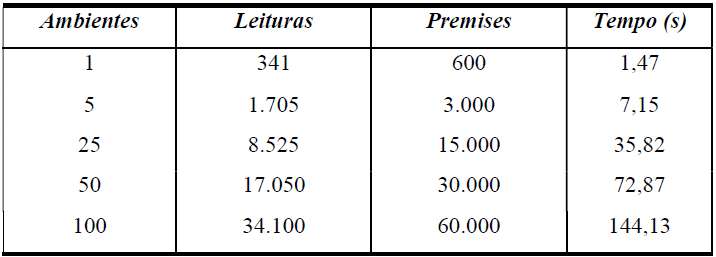
\includegraphics[width=.75\textwidth]{../figures/teste_pon_iot.png}
  \caption{Resultados de testes do PON C\# IoT}
  \caption*{Fonte: \citeonline{msc_oliveira_2019}}
  \label{fig:teste_pon_iot}
\end{figure}

\subsection{\textit{Framework} PON Elixir/Erlang}

Esta materialização chamada \textit{Framework} PON Elixir/Erlang é fruto dos
esforços de mestrado de \citeonline{msc_negrini_2019}, sendo proposta com o
objetivo de aproveitar os conceitos de desacoplamento e, portanto, potencial
paralelização das entidades do PON em conjunto ao modelo de atores da
arquitetura Erlang \cite{msc_negrini_2019}.

Em termos de paradigma, a linguagem Elixir/Erlang segue os princípios do
Paradigma Funcional (PF) associado com o Paradigma Orientado a Atores (POA).
Nesta materialização é introduzido uma implementação na qual os elementos do PON
são modelados por meio de atores. O modelo de atores pode ser definido como uma
extensão dos modelos modulares declarativos ou imperativos, com a passagem
assíncrona de mensagens entre os agentes computacionais elaborados
declarativamente \cite{msc_negrini_2019}.

No \textit{Framework} PON Elixir/Erlang, tanto os elementos da base de fatos
(\textit{i.e.}, \textit{FBEs}, \textit{Attributes} e \textit{Methods}), quanto
suas condições lógico-causais (\textit{i.e.},\textit{Rules},
\textit{Conditions}, \textit{Premises}) e ativadores
(\textit{i.e.},\textit{Actions} e \textit{Instigations}) são desmembrados em
vários atores, enquanto as notificações são implementadas por meio de mensagens
assíncronas, de modo que cada ator carrega uma pequena parte do fluxo de
processamento, cunhando assim micro-atores \cite{msc_negrini_2019}. Um
detalhamento dessa implementação é apresentado por meio da modelagem em UML
apresentada na Figura \ref{fig:pon_elixir_uml}.

\begin{figure}[!htb]
  \centering
  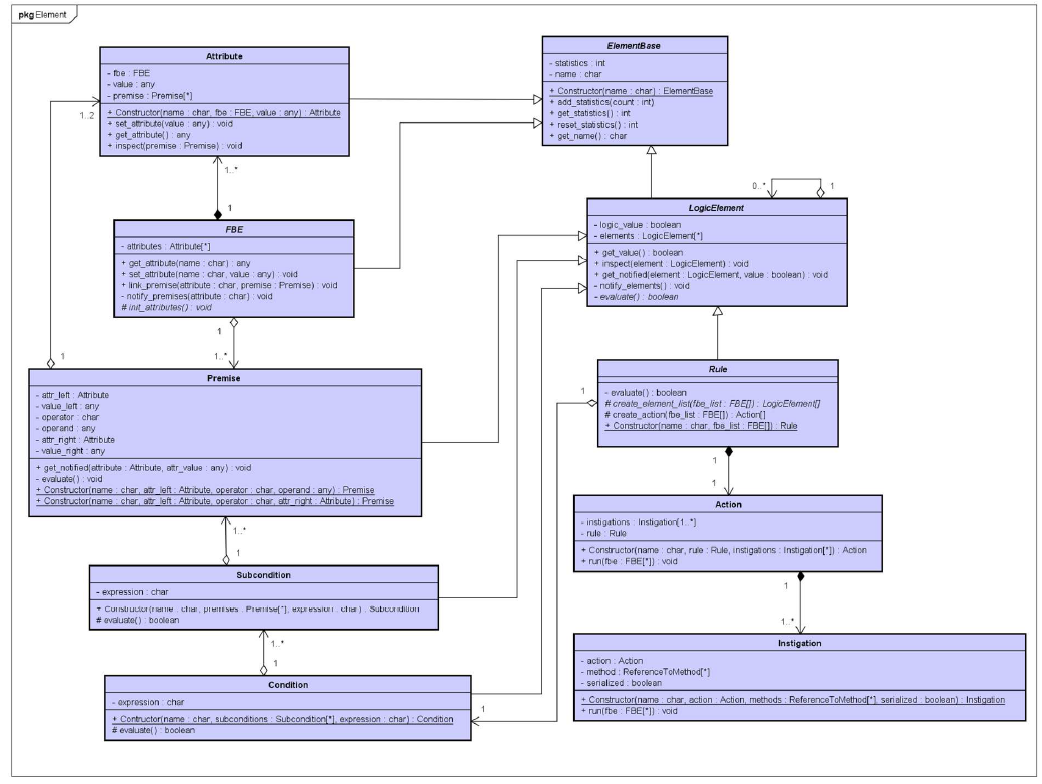
\includegraphics[width=0.9\textwidth]{../figures/pon_elixir_uml.png}
  \smallskip
  \caption{Modelagem UML dos elementos do PON enquanto mircro-atores}
  \caption*{Fonte: \citeonline{msc_negrini_2019}}
  \label{fig:pon_elixir_uml}
\end{figure}
\FloatBarrier

A utilização do \textit{Framework} PON Elixir/Erlang é exemplificada por meio da
implementação de um conjunto de \textit{FBE} e \textit{Rule} bastante simples,
conforme descrito no Código \ref{cod:fbe_negrini}, e implementado com o
\textit{framework} no Código \ref{cod:negrini_rule}. Neste exemplo é descrito um
\textit{FBE} com apenas um \textit{Attribute} \textit{atValue}, e uma
\textit{Rule} que altera o seu valor para 3 quando seu valor é 5, conforme a
\textit{Condition} descrita. Esse exemplo ilustra a utilização da especialização
de \textit{NOP.Element.FBE} e \textit{NOP.Element.Rule} para a implementação das
entidades do PON.

\begin{lstlisting}[language=C++, caption={Exemplo descrito em \textit{FBE} e \textit{Rule}},
label = {cod:fbe_negrini}, float=htb,
source = {Fonte: Autoria própria}
]
fbe Dummy
  public integer atValue = 0
  private method change_value_to_3
    attribution
      this.atValue = 3
    end_attribution
  end_method
  rule rlExample
    condition
      premise prExample
        this.atValue == 5
      end_premise
    end_condition
    action sequential
      instigation sequential
        call this.change_value_to_3()
      end_instigation
    end_action
  end_rule
end_fbe
\end{lstlisting}

\begin{lstlisting}[language = elixir, caption = {Exemplo de implementação de \textit{Rule} como especialização de \textit{NOP.Element.Rule}}, %float=htb,
    source = {Adaptado de \citeonline{msc_negrini_2019}}, label = {cod:negrini_rule}, float=htb]
defmodule NOP.Element.FBE_dummy do
  use NOP.Element.FBE

  defp int_attribuges() do
    %{:value => 0}
  end

  def change_value_to_3(fbe) do
    NOP.Service.FBE.set_attribute(fbe, :value, 3)
  end
end

defmodule NOP.Element.Rule_example do
  use NOP.Element.Rule

  defp create_element_list([fbe]) do
    premise = NOP.Service.Premise.create_premise(
      "NOP.element.premise", fbe, :value, :EQ, 5)
    [premise]
  end

  defp create_instigation_list([fbe]) do
    [{NOP.Element.FBE_dummy, :change_value_to_3, [fbe]}]
  end

end
\end{lstlisting}
\FloatBarrier

Para a validação deste \textit{framework} foi escolhida uma aplicação de
Controle de Tráfego Automatizado (CTA)\footnote{Maiores detalhes sobre esta
aplicação podem ser encontrados em \cite{renaux_2015}}. O objetivo do CTA é
simular o tráfego de uma área urbana e aplicar diferentes estratégias de
controle automatizado de tráfego, de modo a avaliar o desempenho computacional
conforme a estratégia \cite{msc_negrini_2019}. Os testes foram realizados com o
objetivo de avaliar a carga nos núcleos do processador em diferentes ambientes,
com 2, 4, 8 e 16 núcleos. Esses ambientes são identificados na Figura
\ref{fig:ambientes_elixir}.

\begin{figure}[!htb]
  \centering
  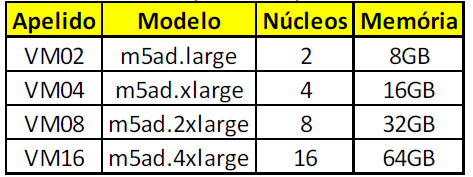
\includegraphics[width=0.65\textwidth]{../figures/maquinas_elixir.png}
  \smallskip
  \caption{Detalhamento dos ambientes do experimento do \textit{Framework} PON
    Elixir/Erlang} \caption*{Fonte: \citeonline{msc_negrini_2019}}
  \label{fig:ambientes_elixir}
\end{figure}

As Figuras \ref{fig:vm02}, \ref{fig:vm04}, \ref{fig:vm08} e \ref{fig:vm16}
exibem a taxa média de ocupação por núcleo e tempo total de execução do
experimento para cada um dos ambientes. Estes resultados apresentam uma
expressiva redução do tempo de execução conforme são acrescidos núcleos aos
ambientes, bem como apresentam que a taxa de ocupação dos núcleos se manteve
balanceada durante a simulação, demonstrando que a execução lógico-causal foi
distribuída com um bom nível de balanceamento entre os núcleos
\cite{msc_negrini_2019}.

\begin{figure}[!htb]
  \centering
  \begin{minipage}{.5\textwidth}
    \centering
    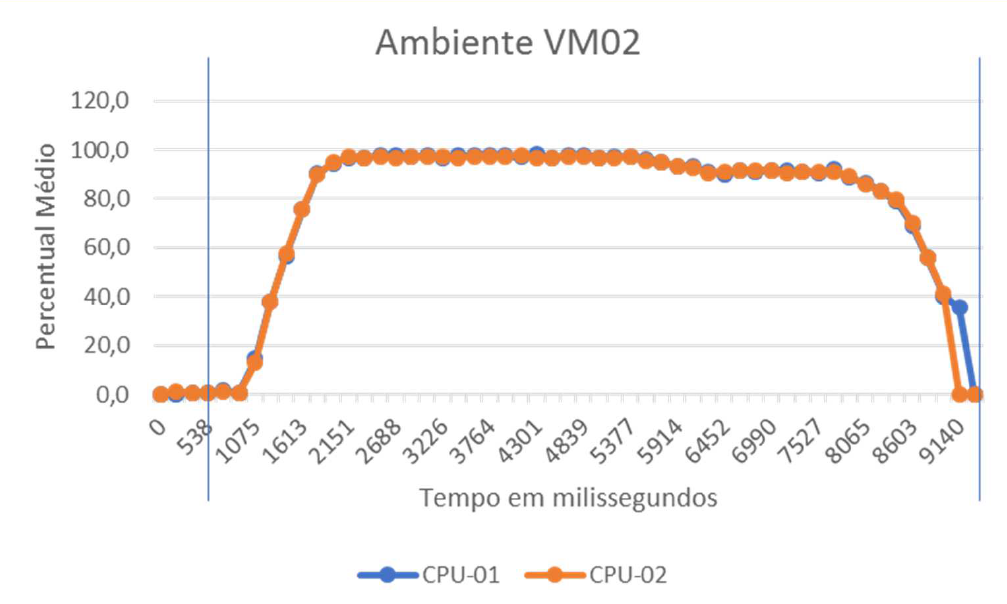
\includegraphics[width=\linewidth]{../figures/vm02.png}
    \smallskip
    \captionof{figure}{Taxa média de ocupação por núcleo em ambiente VM02}
    \captionof{figure}*{Fonte: \citeonline{msc_negrini_2019}}
    \label{fig:vm02}
  \end{minipage}%
  \begin{minipage}{.5\textwidth}
    \centering
    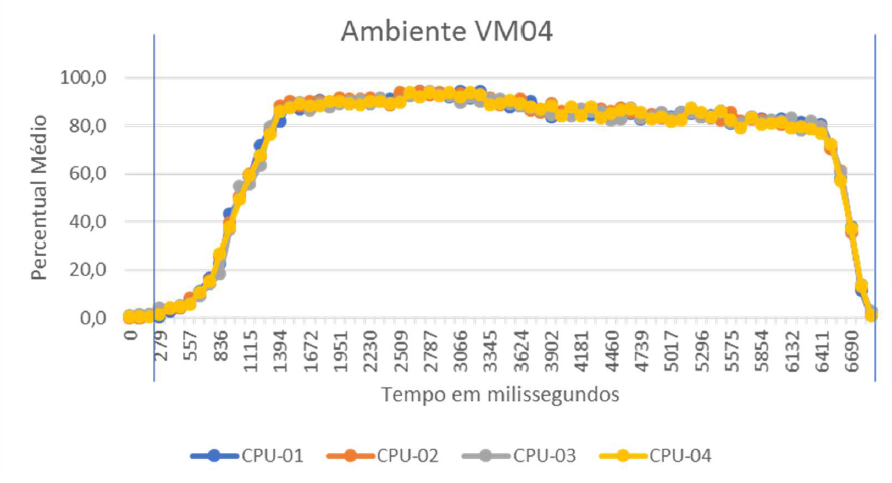
\includegraphics[width=\linewidth]{../figures/vm04.png}
    \smallskip
    \captionof{figure}{Taxa média de ocupação por núcleo em ambiente VM02}
    \captionof{figure}*{Fonte: \citeonline{msc_negrini_2019}}
    \label{fig:vm04}
  \end{minipage}
\end{figure}

\begin{figure}[!htb]
  \centering
  \begin{minipage}{.5\textwidth}
    \centering
    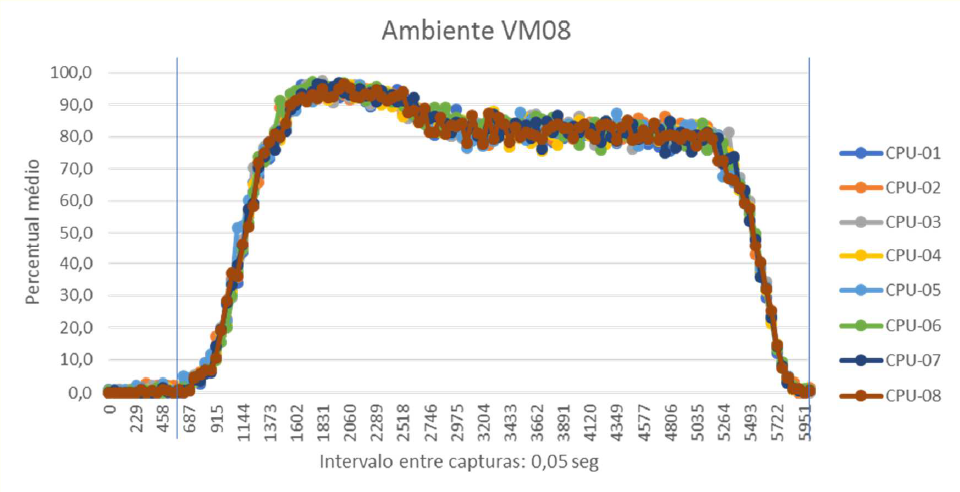
\includegraphics[width=\linewidth]{../figures/vm08.png}
    \smallskip
    \captionof{figure}{Taxa média de ocupação por núcleo em ambiente VM08}
    \captionof{figure}*{Fonte: \citeonline{msc_negrini_2019}}
    \label{fig:vm08}
  \end{minipage}%
  \begin{minipage}{.5\textwidth}
    \centering
    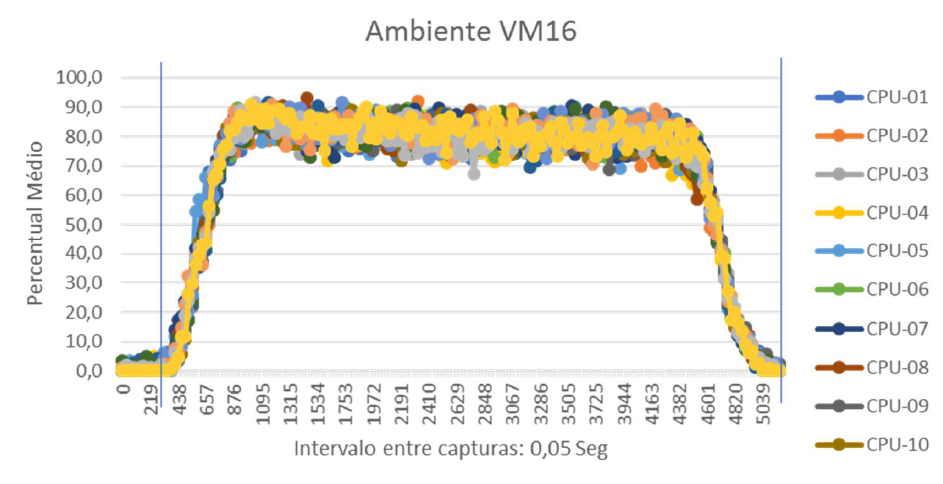
\includegraphics[width=\linewidth]{../figures/vm16.png}
    \smallskip
    \captionof{figure}{Taxa média de ocupação por núcleo em ambiente VM16}
    \captionof{figure}*{Fonte: \citeonline{msc_negrini_2019}}
    \label{fig:vm16}
  \end{minipage}
\end{figure}

\FloatBarrier

\citeonline{doc_Schutz_2019} também utilizou o \textit{Framework} PON
Elixir/Erlang para a execução da RNA MLP para a função XOR em NeuroPON. Para
isto o código foi desenvolvido espelhando-se no experimento realizado com o
\textit{Framework} PON C++ 3.0. A aplicação desenvolvida foi executada em quatro
ambientes diferentes, com 1, 2, 4 e 8 \textit{cores} cada respectivamente.
Conforme os resultados apresentados na Figura \ref{fig:neuropon_elixir},
observa-se que a execução no ambiente com \textit{octa core} apresenta uma
redução de 94\% no tempo de execução quando comparado ao ambiente \textit{mono
core}. 

\begin{figure}[!htb]
  \centering
  \includegraphics[width=0.8\textwidth]{../figures/neuropon_elixir.png}
  \smallskip
  \caption{Tempos médios de execução NeuroPON de uma RNA MLP para a função XOR
  no \textit{Framework} PON Elixir/Erlang} \caption*{Fonte:
  \citeonline{doc_Schutz_2019}}
  \label{fig:neuropon_elixir}
\end{figure}

Isto posto, é possível afirmar que o \textit{Framework} PON Elixir/Erlang é de
grande valia para a execução da NeuroPON, obtendo resultados muito superiores
(em termos de benefícios da paralelização) aos obtidos com a mesma aplicação no
\textit{Framework} PON C++ 3.0. Esse resultado é devido à maneira como o
paralelismo intrínseco ao modelo de atores da linguagem de programação
Elixir/Erlang e implementado por meio do \textit{Framework} PON Elixir/Erlang é
mais eficiente do que o implementado com o \textit{Framework} PON C++ 3.0. Por
fim, esse experimento permite melhor perceber a valia de NeuroPON já em termos
de paralelismo em software \cite{doc_Schutz_2019}.

\subsection{\textit{Framework} PON Akka.NET}\label{sec:akka}

Outro \textit{framework} implementado utilizando o modelo de atores, como
utilizado no \textit{Framework} Elixir/Erlang, mas de maneira um tanto mais
prototipal, é o \textit{Framework} PON Akka.NET, no qual o trabalho das
entidades do PON é distribuído em atores. A Figura \ref{fig:akka_actor} ilustra
a estrutura do modelo de atores em Akka.NET. Os atores criados pela aplicação
são criados sobre o endereço \textit{/root/user}, enquanto os atores criados
automaticamente pelo sistema são criados em \textit{/root/system}. Todos os
atores são acessíveis por seu endereço, mesmo em sistemas distribuídos
\cite{martini_2019}.

\begin{figure}[!htb]
  \centering
  \includegraphics[width=0.8\textwidth]{../figures/atores_akka.png}
  \smallskip
  \caption{Estrutura de atores em Akka.NET}
  \caption*{Fonte: \citeonline{martini_2019}}
  \label{fig:akka_actor}
\end{figure}

Os atores se comunicam entre si por meio de um sistema de mensagens. Cada ator
possui uma referência aos atores que precisam receber suas mensagens. As
notificações do PON são implementadas por meio deste mecanismo de mensagens
\cite{martini_2019}. A mesma aplicação do portão eletrônico, descrita em
detalhes na Seção \ref{sec:csharp_java}, foi desenvolvida com este \textit{framework}.
O diagrama do modelo de atores para esta aplicação é mostrado na Figura
\ref{fig:akka_portao}.

\begin{figure}[!htb]
  \centering
  \includegraphics[width=0.8\textwidth]{../figures/akka_actor.png}
  \smallskip
  \caption{Modelo de atores na aplicação do portão eletrônico em Akka.NET}
  \caption*{Fonte: \citeonline{martini_2019}}
  \label{fig:akka_portao}
\end{figure}

Ainda em termos de códigos, em um momento posterior, aquelas entidades criadas,
conforme ilustrado no Código \ref{cod:akka_create}, precisam ser conectadas de
forma a passar as referências para o processo de envio de mensagens do Akka.NET,
sendo tal processo ilustrado no Código \ref{cod:akka_link}.

\begin{lstlisting}[language = csh, caption = {Criação de atores em Akka.NET}, %float=htb,
source = {Adaptado de \citeonline{martini_2019}}, label = {cod:akka_create}, language={csh}]
IActorRef FBEGateActor = NOPActorSystem.ActorOf(Props.Create(() ->
    new FBEGate()), "FBEGateActor");
IActorRef FBERemoteControlActor = NOPActorSystem.ActorOf(Props.Create(() ->
    new FBERemoteControl()), "FBERemoteControlActor");
IActorRef PremisseIsClosedActor = NOPActorSystem.ActorOf(Props.Create(() ->
    new PremisseIsClosed()), "PremisseIsClosedActor");
IActorRef PremisseIsOpenActor = NOPActorSystem.ActorOf(Props.Create(() ->
    new PremisseIsOpen()), "PremisseIsOpenActor");
IActorRef PremiseChangeStateActor = NOPActorSystem.ActorOf(Props.Create(() ->
    new PremiseChangeState()), "PremiseChangeStateActor");
IActorRef ConditionCloseGateActor = NOPActorSystem.ActorOf(Props.Create(() ->
    new ConditionCloseGate()), "ConditionCloseGateActor");
IActorRef ConditionOpenGateActor = NOPActorSystem.ActorOf(Props.Create(() ->
    new ConditionOpenGate()), "ConditionOpenGateActor");
IActorRef ConditionSateChangedActor = NOPActorSystem.ActorOf(Props.Create(() ->
    new ConditionSateChanged()), "ConditionSateChangedActor");
\end{lstlisting}

\begin{lstlisting}[language = csh, caption = {Conexão entre atores em Akka.NET}, %float=htb,
source = {Adaptado de \citeonline{martini_2019}}, label = {cod:akka_link}, language={csh}]
var FBEGateActorTask1 = FBEGateActor.Ask(
    new ActorReference(ActorRefType.PremisseIsClosedRef, PremisseIsClosedActor));
var FBEGateActorTask2 = FBEGateActor.Ask(
    new ActorReference(ActorRefType.PremisseIsOpenRef, PremisseIsOpenRefActor));
var FBERemoteControlActorTask1 = FBERemoteControlActor.Ask(
    new ActorReference(ActorRefType.PremisseChangeStateRef, PremisseChangeStateActor));
var PremisseIsOpenActorTask1 = PremisseIsOpenActor.Ask(
    new ActorReference(ActorRefType.ConditionCloseGateRef, ConditionCloseGateActor));
var PremisseChangeStateActorTask1 = PremiseChangeStateActor.Ask(
    new ActorReference(ActorRefType.ConditionOpenGateRef, ConditionOpenGateActor));
var PremisseChangeStateActorTask2 = PremiseChangeStateActor.Ask(
    new ActorReference(ActorRefType.ConditionCloseGateRef, ConditionCloseGateActor));
var PremisseChangeStateActorTask3 = PremiseChangeStateActor.Ask(
    new ActorReference(ActorRefType.ConditionOpenGateRef, ConditionOpenGateActor));
var ConditionCloseGateActorTask1 = ConditionCloseGateActor.Ask(
    new ActorReference(ActorRefType.FBEGateRef, FBEGateActor));
var ConditionCloseGateActorTask2 = ConditionCloseGateActor.Ask(
    new ActorReference(ActorRefType.FBERemoteControlRef, FBERemoteControlActor));
var ConditionOpenGateActorTask1 = ConditionOpenGateActor.Ask(
    new ActorReference(ActorRefType.FBEGateRef, FBEGateActor));
var ConditionOpenGateActorTask2 = ConditionOpenGateActor.Ask(
    new ActorReference(ActorRefType.FBERemoteControlRef, FBERemoteControlActor));
var ConditionStateChangedActorTask1 = ConditionStateChangedActor.Ask(
    new ActorReference(ActorRefType.FBERemoteControlRef, FBERemoteControlActor));
\end{lstlisting}

O desempenho deste \textit{framework} é analisado comparando com a aplicação
utilizando o \textit{Framework} PON C++ 3.0. Os resultados da Figura
\ref{fig:result_akka} mostram que com menos atores o desempenho é inferior.
Problemas de alocação de memória do \textit{Framework} PON C++ 3.0 limitaram o
teste a um máximo de 7200 atores, não permitindo uma comparação com um maior
número de atores, no qual o \textit{Framework} Akka.NET tenderia a apresentar
resultados melhores \cite{martini_2019}.

\begin{figure}[!htb]
  \centering
  \includegraphics[width=0.8\textwidth]{../figures/result_akka.png}
  \smallskip
  \caption{Comparação entre o \textit{Framework} PON Akka.NET e C++ 3.0}
  \caption*{Fonte: \citeonline{martini_2019}}
  \label{fig:result_akka}
\end{figure}

\subsection{Reflexões sobre os \textit{frameworks} do PON}\label{sec:reflex}

Esta subseção traz um arrazoado sobre os \textit{frameworks} do PON para
\textit{software} apresentados nas subseções anteriores. Tal arrazoado analisa
estas materializações sobre distintos pontos de vista, nas suas três subseções
que seguem,

\subsubsection{\textit{Frameworks} do PON vis-à-vis sua teoria}

O grande número de materializações disponíveis do PON é interessante, pois
permite a aplicação do PON em diversos ambientes diferentes. Entretanto, cada
uma dessas materializações contempla apenas alguns dos conceitos e propriedades
do PON introduzidos em seções prévias deste presente capítulo.

Os conceitos e o potencial de propriedades que são implementados em cada uma
destas materializações são apresentados nas tabelas abaixo. A Tabela
\ref{tab:elementares} relaciona quais propriedades elementares alcançam seus
potenciais, abordadas na Seção \ref{sec:estado_arte_pon}, são contempladas em
cada uma das materializações do PON, do mesmo modo que a Tabela
\ref{tab:conceitos} relaciona os conceitos apresentados na Seção
\ref{sec:conceitos_pon}. 
%Nessas tabelas o símbolo (\checkmark) indica que
%contempla completamente e (\textasciitilde) indica que contempla parcialmente.

\begin{table}[!htb]
  \centering
  \caption{Propriedades elementares contempladas nas materializações do PON}
  \caption*{Fonte: Autoria própria}
  \label{tab:elementares}
  \smallskip
  \begin{threeparttable}
    \begin{tabularx}{\textwidth}{|l||*{8}{X|}}\hline
      \diagbox{Potencial\\ de propriedade}{Materialização} & 
      Fw. C++ Prot. & Fw. C++ 1.0 & Fw. C++ 2.0 & Fw. C++ 3.0 & Fw. Java /C\# & Fw. C\# IoT & Fw. Elixir & Fw. Akka \\\hline\hline
      \makecell{Programação\\ em alto nível}             & \textasciitilde & \textasciitilde & $\star$ & \textasciitilde & \textasciitilde & \textasciitilde & \textasciitilde & \textasciitilde \\\hline
      \makecell{Paralelismo\\ via desacoplamento}        & & & & \textasciitilde & & \checkmark & \checkmark & \checkmark \\\hline
      \makecell{Distribuição\\ via desacoplamento}       & & & & & & \checkmark & * & * \\\hline
      \makecell{Desempenho\\ via não redundâncias}       & & & \textasciitilde & & \textasciitilde & & & \\\hline
    \end{tabularx}
    \begin{tablenotes}
      \item[\checkmark] Materializa completamente a propriedade
      \item[\textasciitilde] Materializa parcialmente a propriedade
      \item[$\star$] Materializa a propriedade por meio de ferramenta \textit{wizard} \cite{msc_valenca_2012}
      \item[*] A tecnologia de base permite materializar a propriedade,
      entretanto carece de testes para validação
    \end{tablenotes}
  \end{threeparttable}
\end{table}

Pode ser dito que nenhuma das materializações atinge de forma plena o quesito de
programação em alto nível, devido à complexidade do uso dos \textit{frameworks}
que requer que o programador ainda conheça certos detalhes de implementação do
\textit{framework} para implementar a aplicação em PON em si. Isso se dá também
pelas limitações impostas ao se implementar o PON sobre linguagens com base em
outros paradigmas. A programação em alto nível só é atingida de maneira
completamente satisfatória por meio da linguagem de programação do PON (a
LingPON), ainda que em \textit{framework} seja possível alcançar algo similar
conforme observado no prototipal e infindado JuNOC++.

Além dos \textit{frameworks} atuais realmente funcionais/findados não
contemplarem apropriadamente desenvolvimento em alto nível, salvo se usarem uma
interface \textit{wizard} que limitaria criatividade (ainda que certamente úteis
para dados contextos), eles também não contemplam apropriadamente o potencial de
bom desempenho, que seria alcançável pelo evitar implícito de redundâncias
existentes no PON. De fato, dito mais precisamente e pragmaticamente, nenhuma
destas materializações em \textit{frameworks} é capaz de atingir o desempenho
esperado à luz do cálculo assintótico do PON, por se basearem em estruturas de
dados computacionalmente custosas que acabam mascarando a baixa complexidade
assintótica-temporal do PON. Ainda que em \textit{frameworks} não seja possível
escapar do uso destas estruturas de dados, possivelmente elas poderiam ser
mais bem articuladas, mesmo mais do que no \textit{Framework} PON C++ 2.0 que é
o de melhor desempenho até então.

Por fim, apesar de as entidades do PON serem paralelizáveis e mesmo
distribuíveis, graças ao desacoplamento que existe entre elas por definição,
apenas algumas das materializações implementam a potencialidade dessa
propriedade. Ainda, quando isto ocorre, não tem conseguido manter equilíbrio
para com questão de performance. Isso ocorre por dois motivos, os quais seriam
em algo gerenciáveis, mas finalmente não foram gerenciados. Primeiramente, há a
dificuldade de se implementar mecanismos de sincronização entre elementos
paralelizáveis em algumas linguagens de programação, além do alto tempo de
execução associado a estes mecanismos. Do mesmo modo, a distribuição das
entidades é possível, porém também possui um alto custo em tempo de execução
devido aos mecanismos de comunicação entre as entidades, como o uso de mensagens
assíncronas. Desta forma as materializações com paralelismo e distribuição
apresentam desempenho mais baixo.

Além da potencialidade do uso das propriedades elementares do PON, há também os
conceitos de programação ou desenvolvimento em PON que foram tratados na Seção
\ref{sec:conceitos_pon}. Isto dito, a Tabela \ref{tab:conceitos} mostra que
todas as materializações não implementam um ou mais daqueles conceitos
finalmente. Isso pode ser atribuído ao grau de maturidade de cada uma das
materializações, assim como pela dificuldade de se implementar determinados
conceitos em algumas linguagens de programação. De forma geral o
\textit{Framework} PON C++ 2.0 e 3.0 são os que atendem a maior parte destes
conceitos, também devido ao fato que muitos destes conceitos terem sido
introduzidos justamente nos trabalhos que fizeram o desenvolvimento do
\textit{Framework} PON C++ 2.0 \cite{msc_Ronszcka_2012,msc_valenca_2012}.

\begin{table}[!htb]
  \centering
  \caption{Conceitos do PON contemplados nas materializações do paradigma}
  \caption*{Fonte: Autoria própria}
  \label{tab:conceitos}
  \smallskip
\begin{threeparttable}
  \begin{tabularx}{\textwidth}{|l||*{8}{X|}}\hline
    \diagbox{Conceito\\de Programação}{Materialização} 
    & Fw. Prot. & Fw. C++ 1.0 & Fw. C++ 2.0 & Fw. C++ 3.0 & Fw. Java / C\# & Fw. C\# IoT & Fw. Elixir & Fw. Akka \\\hline\hline
    Reatividade das entidades     & \checkmark  & \checkmark     & \checkmark  &
    \checkmark                    & \checkmark  & \checkmark     & \checkmark  &
    \checkmark                                                                                         \\\hline
    Compartilhamento de entidades &             & \checkmark     & \checkmark  &
    \checkmark                    & \checkmark  & \checkmark     & \checkmark  &
    \\\hline
    Renotificações                &             & \checkmark     & \checkmark  &
    \checkmark                    & \checkmark  &                &             &                       \\\hline
    Resolução de conflitos        &             & \checkmark     & \checkmark  &
    \checkmark                    & \checkmark  & \checkmark     &             &
    \\\hline
    \textit{Master Rule}          &             &                & \checkmark  &
    \checkmark                    &             &                &             &                       \\\hline
    Impertinência estática        &             &                & \checkmark  &
    \checkmark                    &             &                &             &                       \\\hline
    Impertinência dinâmica        &             &                &             &
                                  &             & \checkmark     &             &                       \\\hline
    \textit{FBE Rules}            &             &                & \checkmark  &
    \checkmark                    &             &                &             &                       \\\hline
    \textit{FBE} Agregador        &             &                & \checkmark  &
    \checkmark                    &             &                &             &                       \\\hline
    \textit{Formation Rules}      &             &                &             &
                                  &             &                &             &                       \\\hline
    \textit{Keeper}               &             &                & *           &
                                  &             &                &             &                       \\\hline
  \end{tabularx}
  \begin{tablenotes}
    \item[*] Implementado sob a forma de uma adaptação no \textit{framework}
    existente, visto que altera o fluxo tradicional de execução das
    \textit{Rules} do PON \cite{muchalski_2012}
  \end{tablenotes}
\end{threeparttable}
\end{table}

\begin{comment}
Este trabalho se interessa mais nas materializações em software, devido ao seu
maior grau de maturidade, em especial o \textit{Framework} PON C++ 2.0 que é a
materialização com maior grau de maturidade dentre elas
\cite{ronszcka_2017,pat_simao_2017}. Porém, também é importante mencionar os
esforços das materializações em hardware, como: O desenvolvimento do CoPON, um
coprocessador desenvolvido para acelerar a execução de aplicações desenvolvidas
em PON em VHDL; O PON \textit{Hardware} Digital(PON-HD)
\cite{doc_Kerschbaumer_2018}, com a geração de \textit{hardware} digital em VHDL
por meio do código PON em alto nível; \textit{A Notification Oriented Computer
  Architecture} (NOCA) \cite{doc_linhares_2015}, que é uma arquitetura de
computação desenvolvida para a execução de \textit{software} segundo o modelo
computacional do PON, que por sua vez conta com o Simulador NOCA (NOCASim)
\cite{msc_pordeus_2017}, um simulador desenvolvido para simular a NOCA,
facilitando seu estudo e testes. Essas materializações em hardware apresentam,
em alguns casos, desempenho mais satisfatório e paralelismo intrínseco, em
detrimento da facilidade de programação ou desenvolvimento
\cite{doc_ronszcka_2019}.
\end{comment}

Dadas estas reflexões sobre as materializações existentes do PON em termos de
frameworks vis-à-vis a teoria do PON, a seção seguinte apresenta reflexões
específicas com relação os \textit{frameworks} em geral enquanto estado da
técnica, usando como condutor das reflexões o \textit{Framework} PON C++ 2.0,
dado que este é a materialização com maior grau de maturidade dentre os
\textit{frameworks} do PON.

\subsubsection{\textit{Frameworks} do PON enquanto estado da
técnica}\label{sec:reflex_cpp2}

Do ponto de vista de implementação de programas em PON, para a solução de
problemas reais, dentre todas as materializações do PON a mais utilizada ainda é
o \textit{framework} C++ 2.0, devido a seu maior grau de maturidade e
estabilidade entre as materializações desenvolvidas \cite{ronszcka_2017}. Apesar
desta versão de \textit{framework} oferecer todos os recursos necessários para a
aplicação dos conceitos e desenvolvimento de programas no PON, ela ainda
apresenta alguns problemas que dificultam a sua aplicação no desenvolvimento de
um programa no PON. Estes problemas são listados nas seções seguintes, sendo que
se replicam ademais nos demais frameworks

\paragraph*{Verbosidade}

O \textit{framework} C++ 2.0 exige a escrita de uma quantidade muito
significativa de código para se desenvolver uma aplicação básica. Isso vem da
necessidade de se criar muitos métodos diferentes para se inicializar as
diferentes entidades. As construções de objetos são complexas e muitas vezes
exigem múltiplas linhas de código.

Essa verbosidade tenta ser mitigada por meio do uso de \textit{macros}, que são
fragmentos de código aos quais é dado um nome. Quando esse nome é utilizado, ele
é substituído pelo conteúdo da \textit{macro}, expandindo os parâmetros passados
na etapa de compilação. Porém, isso apenas tenta esconder a verbosidade, sem de
fato solucionar o problema em si.

Esta característica de verbosidade foi herdada pelos demais \textit{frameworks}
em geral, exceto pelo todo prototipal JuNOC++.

\paragraph*{Baixa flexibilidade de tipos}

O \textit{Framework} PON C++ 2.0 limita o desenvolvedor ao uso de atributos dos
tipos \textit{integer}, \textit{double}, \textit{bool}, \textit{string}. Em boa
parte dos casos de uso isso pode ser suficiente, mas principalmente quando é
feita a integração com APIs e bibliotecas externas isso pode ser um fator
limitador que dificulta o desenvolvimento de código.

Ainda do ponto de vista de implementação do \textit{framework} em si isso leva a
uma necessidade de duplicação de código muito grande pela necessidade de se
implementar métodos e estruturas de dados especializadas para cada tipo. Isso
causa problemas principalmente para eventual manutenção do código e
implementação de novas funcionalidades, visto que torna mais trabalhoso precisar
replicar alterações idênticas em diversos trechos de código.

Esta característica de baixa flexibilidade foi herdada pelos demais
\textit{frameworks} em geral, com exceção daqueles implementados em linguagem
com tipagem dinâmica, como o \textit{Framework} PON Elixir/Erlang.

\paragraph*{Baixa flexibilidade algorítmica}

Além da baixa flexibilidade de tipos, também cabe uma crítica à flexibilidade
algorítmica, visto que as estruturas de avaliação lógica das \textit{Conditions}
e \textit{Premises} obedecem a uma estrutura rígida com a qual o desenvolvedor
não consegue criar avaliações mais complexas. Por exemplo, não se pode agregar
diversas \textit{Premises} por meio de uma expressão lógica booleana genérica
(\textit{e.g.}, \textit{premise1 and premise2 or (premise3 and not premise5)}),
sendo limitado ao uso de \textit{Conditions} utilizando apenas conjunções ou
apenas disjunções. Isto leva à necessidade de se criar um número muito maior de
entidades, como \textit{Premises} e \textit{Conditions} auxiliares, para se
implementar a condição desejada.

Esta característica de baixa flexibilidade algorítmica foi herdada pelos demais
\textit{frameworks} em geral, exceto pelo todo prototipal JuNOC++.

\paragraph*{Baixa confiabilidade}

A baixa confiabilidade é atribuída à falta de testes realizados sob os
\textit{frameworks} em si. A aplicação de testes unitários em um
\textit{software} é capaz de reduzir significativamente o número de defeitos
durante o seu uso \cite{microsoft_test_2009}.

Nos \textit{frameworks} existentes o único método para se testar possível é por
meio da construção de aplicações completas, que funcionam como testes de
integração. Estes testes são capazes de validar apenas em um contexto limitado
do \textit{software} como um todo, não testando cada parte do \textit{framework}
individualmente sob a perspectiva de testes unitários. Esse método pode ser útil
para validar os conceitos de PON e até mesmo para realizar análises de
desempenho, porém é muito menos eficiente para se encontrar problemas.

Esta característica de verbosidade foi herdada pelos demais \textit{frameworks}
em geral.

\paragraph*{Curva de aprendizado não suave}

Todos esses fatores supracitados contribuem para a construção de um ambiente de
desenvolvimento pouco amigável ou não tão amigável (conforme o ponto de vista)
para a introdução a novos desenvolvedores, restringindo ainda um tanto o
desenvolvimento de aplicações no PON a desenvolvedores mais experientes e com
conhecimento mais profundo do paradigma ou que passem por treinamento para tal.
Tal curva de aprendizado é prejudicial para a popularização do paradigma entre
desenvolvedores, sendo que a intenção sempre foi o PON ser intuitivo.

Ademais, este quadro dado também dificulta a manutenção e melhoria dos códigos,
visto que dado o contexto acadêmico de sua construção, o autor de uma das
versões do \textit{framework} usualmente não contribui mais com seu
desenvolvimento após a finalização dos seus estudos, passando essa
responsabilidade para outro pesquisador e/ou estudante.

\subsubsection{Ponderações gerais sobre a pertinência de \textit{Frameworks} do PON}

Apesar das imperfeições de cada \textit{framework} em si, bem como no tocante ao
aproveitamento das propriedades do PON e mesmo dos próprios conceitos de
programação do PON, eles continuam sendo o estado da técnica em PON. Ademais,
mesmo antes de ser estado da técnica, enquanto estado da arte, os
\textit{frameworks} têm permitido demonstrar vantagens do PON em relação a outros
paradigmas. 

Neste sentido, os \textit{Frameworks} PON C++ 1.0/2.0, Java e C\# permitiram
mostrar um bom equilíbrio de programação em mais alto nível que em programação
imperativa, sem perda importante de performance como ocorre na declarativa
\cite{msc_Banaszewski_2009,henzen_2015,ronszcka_2017}. Por sua vez, o
\textit{Framework} PON C++ 3.0 mostrou a viabilidade de automaticamente obter
balanceamento fino de carga entre núcleos de processamento
\cite{belmonte_2012,belmonte_2016}. 

Ainda, os \textit{Frameworks} PON Erlang/Elixir e Akka.net mostraram a
viabilidade de implicitamente alcançar melhor paralelismo fino em nível de
threads com melhor equilíbrio de carga nos processadores ou núcleos do que suas
tecnologias de atores apenas respectivamente sobre paradigmas funcional e
imperativo \cite{martini_2019,msc_negrini_2019}. Por fim, o prototipal JuNOC++
mostrou a possibilidade de programação em mais alto nível mesmo em âmbito de
\textit{framework} \cite{chierichi_2020}. 

Em suma, os \textit{frameworks} ainda são tecnologias importantes para o PON e
podem melhorar ao aproveitamento das propriedades e dos conceitos de programação
do PON desde que seus benefícios sejam articulados e suas deficiências em algo
mitigadas. Dadas estas reflexões sobre a pertinência de \textit{frameworks} PON
enquanto estado da técnica, em subseção seguinte apresenta a Tecnologia LingPON
enquanto estado da arte. De antemão, a Tecnologia LingPON permite programar em
alto nível e, dentre outros, gerar código para a maioria dos \textit{frameworks},
permitindo assim seus usos em altíssimo nível de desenvolvimento. 

Por fim e em tempo, este trabalho se interessa nas materializações puramente em
\textit{software}, conforme já salientado. Porém, apenas para fins de registro e
divulgação, também é pertinente mencionar os esforços das materializações do PON
para \textit{hardware} e que se correlacionam em algo com as soluções em \textit{software}, como: 

\begin{itemize}
  \item O PON \textit{Hardware} Digital (PON-HD), que permite a geração de
  \textit{hardware} digital via VHDL por meio do código PON em considerável alto
  nível. PON-HD passou por etapas prototipais a até alcançar um conjunto de
  componentes em VHDL que se constituem em uma forma de framework para tal
  \cite{doc_Kerschbaumer_2018,kerschbaumer_2018_2,kerschbaumer_2018_1}.
  \item O CoPON, um coprocessador em VHDL desenvolvido para acelerar a execução
  de aplicações desenvolvidas em \textit{Framework} PON C++ 1.0 adaptado para
  tal. A construção do CoPON inspirou-se em versões prototipais do PON-HD
  \cite{msc_Peters_2012,peters_2012}; 
  \item A ArqPON ou NOCA (\textit{Notification Oriented Computer Architecture}), que é
  uma arquitetura de computação desenvolvida para a execução de
  \textit{software} segundo o modelo computacional do PON, tendo \textit{assembly}
  próprio para composição de \textit{software} em si
  \cite{doc_linhares_2015,linhares_2020}.
  \item O Simulador ArqPON (ou NOCASim), um simulador desenvolvido para simular
  a NOCA, facilitando seu estudo e testes \cite{msc_pordeus_2017,linhares_2020}. 
\end{itemize}

Em suma, essas materializações em \textit{hardware} apresentam geralmente
desempenho mais satisfatório e paralelismo intrínseco, em detrimento da
facilidade de programação ou desenvolvimento \cite{doc_ronszcka_2019}.
Entretanto, isto é resolvido pelo fato da Tecnologia LingPON permitir programar
em alto nível e também gerar código para estas soluções envolvendo em
\textit{hardware} do PON, permitindo assim seus usos em altíssimo nível de
desenvolvimento, conforme será vista na próxima subseção.


\subsection{Tecnologia LingPON}\label{sec:lingpon}

Além das materializações por meio de implementação sob a forma de
\textit{framework} em outras linguagens de programação para \textit{software},
bem como as supracitadas soluções em \textit{hardware}, o PON também conta com
sua própria linguagem de programação, a LingPON. Com a LingPON é possível
desenvolver programas diretamente em PON, utilizando a sua sintaxe e linguagem
própria. Esse código então passa por um processo de compilação capaz de gerar um
código alvo para os \textit{frameworks} disponíveis. Em tempo, LingPON e sua
tecnologia de compilação ímpar tem sido chamada de Tecnologia LingPON
\cite{doc_ronszcka_2019}.

A Tecnologia LingPON já possui diferentes versões: Tecnologia LingPON
Prototipal, Tecnologia LingPON 1.X (1.0 e 1.2), Tecnologia LingPON HD 1.0,
Tecnologia LingPON 2.0, cada qual com seu sistema de compilação e sua linguagem
de programação da tecnologia. No caso da Tecnologia LingPON 2.0, a linguagem de
programação LingPON 2.0 também é chamada de NOPL (\textit{Notification Oriented
Programing Language}) \cite{doc_ronszcka_2019}. Ainda, tal tecnologia já tem
mesmo a proposta e protótipo de uma segunda linguagem de programação, a NOPLite
\cite{chierichi_2020}. Esta última seguiria um padrão mais direto e pontual
especialmente voltada para especialistas do PON \cite{doc_ronszcka_2019}.

Como exemplo da construção de programas e sintaxe de alto nível em LingPON 2.0
ou NOPL, o Código \ref{cod:lingpon} apresenta o modelo de criação de um
\textit{FBE} e uma \textit{Rule} para um exemplo do sensor previamente
introduzido na Figura \ref{fig:nop_rule} da Seção \ref{sec:pon}. Maiores
detalhes sobre a sintaxe e utilização desta linguagem podem ser consultados em
\cite{doc_ronszcka_2019}.

\begin{lstlisting}[caption = {Exemplo de construção de entidades na LingPON 2.0}, float=htb,
  source = {Fonte: Autoria própria}, language=nopl,
  label = {cod:lingpon}]
  fbe Sensor
    public boolean atIsRead = false
    public boolean atIsActivated = false
    private method mtProcess
      attribution
        this.atIsRead = true
        this.atIsActivated = false
      end_attribution
    end_method
    rule rlSensor
      condition
          premise prIsActivated
            this.atIsActivated == true
          end_premise
          and
          premise prDebug
            this.prIsNotRead == false
          end_premise
      end_condition
      action sequential
          instigation sequential
            call this.mtProcess()
          end_instigation
      end_action
    end_rule
  end_fbe
\end{lstlisting}

Isto posto, para possibilitar o desenvolvimento de cada Tecnologia LingPon,
destacando a 1.X e 2.0, foi proposto um novo método para uniformizar o processo
de construção de linguagens e compiladores específicos para o PON em plataformas
distintas. Para esse método foi dado o nome de MCPON \cite{doc_ronszcka_2019}.

Em suma, o MCPON define um conjunto de diretrizes e regras para a construção de
uma representação intermediária adequada para programas em PON. Esta forma
intermediária é dada por meio de um grafo, o Grafo PON, que permite representar
apropriadamente um programa em PON. O MCPON institui um sistema completo para o
processo de compilação, usando o Grafo PON. Nesse âmbito, a Figura
\ref{fig:mcpon} ilustra as cinco etapas do método MCPON
\cite{doc_ronszcka_2019}.

\begin{figure}[!htb]
  \centering
  \includegraphics[width=0.8\textwidth]{../figures/metodo_mcpon.png}
  \smallskip
  \caption{Método MCPON}
  \caption*{Fonte: \citeonline{doc_ronszcka_2019}}
  \label{fig:mcpon}
\end{figure}

A primeira etapa do MCPON visa construir linguagens particulares para o PON. A
segunda etapa visa definir o processo de construção de instâncias do Grafo PON.
A terceira etapa visa a construção de otimizadores. A quarta etapa visa a
tradução dos grafos em códigos-alvo tanto em linguagens quanto em plataformas
distintas. Por fim, a quinta etapa visa a construção de validadores
\cite{doc_ronszcka_2019}.

No método MCPON, o Grafo PON é o elemento central, especialmente desenvolvido
para a criação de linguagens e compiladores particulares ao PON. Nesse sentido,
o Grafo PON serve, então, como uma representação intermediária para o mapeamento
completo de programas PON e, principalmente, mantém a essência do PON, a qual é
orientada a entidades notificantes desacopladas \cite{doc_ronszcka_2019}. De
maneira gráfica, uma instância do Grafo PON é demonstrada na Figura
\ref{fig:grafo_pon}, ilustrando a relação entre as diversas entidades do PON
na estrutura do Grafo PON \cite{msc_negrini_2019}.

\begin{figure}[!htb]
  \centering
  \includegraphics[width=\textwidth]{../figures/grafo_pon_negrini.png}
  \smallskip
  \caption{Estrutura do Grafo PON}
  \caption*{Fonte: \citeonline{msc_negrini_2019}}
  \label{fig:grafo_pon}
\end{figure}

Essa etapa de compilação intermediária por meio do Grafo PON permite  a geração
de códigos específicos para diferentes alvos com base em um único código-fonte
em LingPON, processo que é ilustrado na Figura \ref{fig:sistema_compilacao}.
Neste âmbito, a Tecnologia LingPON é capaz de gerar código para as
implementações de \textit{framework} do PON ou mesmo código notificante
específico em linguagens como C e C++. 

\begin{figure}[!htb]
  \centering
  \includegraphics[width=0.8\textwidth]{../figures/sistema_compilacao.png}
  \smallskip
  \caption{Sistema de compilação do PON}
  \caption*{Fonte: \citeonline{doc_ronszcka_2019}}
  \label{fig:sistema_compilacao}
\end{figure}

Esta geração de código notificante específico em C/C++ apresenta excelente
resultados de performance, por evitar justamente as sobrecargas de processamento
com estruturas de dados dos frameworks, respeitando assim o cálculo assintótico
do PON \cite{ronszcka_2017,doc_ronszcka_2019,oshiro_2021}. Ainda, já se começa
ter soluções com algum paralelismo em \textit{multicore}
\cite{doc_ronszcka_2019,martini_2021}.

No âmbito da geração de código notificante específico em C++ com a LingPON 2.0,
foram ainda criados os geradores de código LingPON \textit{Static} (Estático) e
LingPON \textit{Namespaces} (Espaço de Nomes). O gerador de código
\textit{LingPON Static} apresenta desempenho ainda melhor que os outros
geradores para C++ notificantes, por meio do uso de classes estáticas.
Entretanto, essa versão dificultou a integração com outros códigos legados em
C++, devido ao código ser orientado a atributos estáticos, que inviabilizam a
integração com código usual \cite{schutz_2015}.

Já o gerador de código \textit{LingPON Namespaces}, tal qual LingPON
\textit{Static}, buscava eliminar a sobrecarga causada pelo uso de classes e
objetos do POO em C++ específico, mas agora tratando as entidades por meio dos
espaços de nomes (\textit{namespaces}) e não código estático. Esta versão
LingPON \textit{Namespaces} consegue manter o baixo tempo de processamento da versão
estática, ao mesmo tempo que resolve os problemas de integração presentes na
mesma justamente \cite{athayde_2016}.

Ademais, também é possível gerar código \textit{assembly} para a NOCA e VHDL em
PON-HD, conforme ilustrado na Figura \ref{fig:sistema_compilacao}. No que diz
respeito aos \textit{targets} ilustrados na Figura \ref{fig:sistema_compilacao},
justamente, além destes, ainda é possível gerar código específico para os quase todos os
\textit{frameworks} apresentados na Seção \ref{sec:frameworks}, com exceção do
\textit{Framework} Akka.NET e do \textit{Framework} PON C++ Prototipal.

Tudo isto considerado, ainda que a LingPON possibilite o desenvolvimento de
\textit{software} em alto nível e diretamente em PON, é difícil fazer a
construção de aplicações completas com a LingPON, principalmente devido ao seu
estado ainda prototipal vis-à-vis os \textit{frameworks} PON. Neste sentido,
aplicações em PON podem depender de acesso a arquivos, protocolos de rede e
interfaces de usuário, sendo estas funcionalidades não cobertas pela LingPON.
Apesar da LingPON oferecer algumas ferramentas para realizar a interface com
código externo em outras linguagens, seu uso ainda é limitado. Nesses contextos,
é mais vantajosa a utilização dos \textit{frameworks} que permitem uma
integração mais fácil com outras bibliotecas externas, sendo que o uso pode ser
feito associado com a LingPON no tocante a escrita dalógica principal de
\textit{FBEs} e \textit{Rules}.

\clearpage
\section{Método de teste de \textit{software} para o PON}\label{sec:test_pon}

Dada que uma das propostas deste trabalho é utilizar o método TDD no
desenvolvimento de um \textit{framework} para o PON, é importante destacar os
esforços de \citeonline{msc_Kossoski_2015} no desenvolvimento de um método de
teste de \textit{software} para o PON. Este método proposto aplica-se tanto nas
fases de teste unitário quanto de teste de integração, apresentados nas Seções
\ref{sec:unit_pon} e \ref{sec:int_pon} respectivamente.

\subsection{Teste unitário em PON}\label{sec:unit_pon}

O teste unitário considera a menor unidade ou trecho de código que pode ser
testada em uma aplicação. No contexto do PON, foram elaboradas estratégias para
o teste de \textit{Premises}, \textit{Conditions}, \textit{Subconditions},
\textit{Rules} e \textit{Methods} dos \textit{FBEs}, enquanto os
\textit{Attributes}, \textit{Actions} e \textit{Instigations}, por sua vez, não
precisam passar por testes unitários. Do ponto de vista de teste, isso é devido
ao fato dos \textit{Attributes} representarem apenas uma declaração de estado,
enquanto \textit{Actions} e \textit{Instigations} têm sempre o mesmo
comportamento garantido por definição \cite{msc_Kossoski_2015}.

São apresentadas abordagens distintas para o desenvolvimento de testes para cada
uma das entidades:

\begin{itemize}
  \item \textit{Premise}: determinação de classes de equivalência e análise de
        valores limites que exercitem o operador lógico e os \textit{Attributes}
        avaliados \cite{msc_Kossoski_2015}.
  \item \textit{Conditions e Subconditions}: são requeridos casos de teste que
        exercitem os estados das \textit{Premises} e \textit{Subconditions}
        avaliadas na sua operação lógica \cite{msc_Kossoski_2015}.
  \item \textit{Rules}: são considerados apenas os estados da
        \textit{Condition}, que pode estar aprovada ou não aprovada
        \cite{msc_Kossoski_2015}.
  \item \textit{Methods} dos \textit{FBEs}: exercitar os parâmetros de entrada
        do \textit{Method} e configuração de outros \textit{Attributes} ou
        estados de objetos que serão utilizados \cite{msc_Kossoski_2015}.
\end{itemize}

Como exemplo, considera-se uma \textit{Premise} \textit{prTest} que avalia se
dado \textit{Attribute} \textit{atTest} é menor ou igual a 800. A determinação
de classes de equivalência define uma classe de valores válidos e uma classe de
valores inválidos para o \textit{Attribute} desta \textit{Premise}, conforme
apresentado na Figura \ref{fig:classe_equivalencia}. Ainda, com o levantamento
das classes de equivalência, podem ser planejados os devidos casos de testes
para esta \textit{Premise}, conforme apresentados na Tabela \ref{tab:test_case}

\begin{figure}[!htb]
  \centering
  \includegraphics[width=0.7\textwidth]{../figures/classes_equivalencia.png}
  \smallskip
  \caption{Classes de equivalência e análise de valores limite}
  \caption*{Fonte: \citeonline{msc_Kossoski_2015}}
  \label{fig:classe_equivalencia}
\end{figure}


\begin{table}[!htb]
  \centering
  \caption{Caso de teste prara \textit{Premise}} \caption*{Fonte: Adaptado de
    \citeonline{msc_Kossoski_2015}}
  \label{tab:test_case}
  \smallskip
  \begin{tabularx}{\textwidth}{|l|*{6}{X|}}\hline
    Caso de teste & Valor de \textit{atTest} & \makecell{Saída esperada ou\\ comportamento esperado}    \\\hline
    1 & 799 & Aprova a \textit{Premise} \\ \hline
    2 & 800 & Aprova a \textit{Premise} \\ \hline
    3 & 801 & Não aprova a \textit{Premise} \\ \hline
    4 & 802 & Não aprova a \textit{Premise} \\ \hline
  \end{tabularx}
\end{table}

\FloatBarrier

Para cada unidade (\textit{i.e.}, \textit{Premises}, \textit{Conditions},
\textit{Rules}, \textit{Methods}) é necessário o levantamento dessas classes de
equivalência que permitem planejar os casos de teste para cada uma delas. A
Figura \ref{fig:unit_pon} apresenta uma visão expandida da fase de testes
unitários, que engloba o planejamento e geração dos casos de testes, execução
dos casos de teste e análise dos resultados dos testes unitários
\cite{msc_Kossoski_2015}.

\begin{figure}[!htb]
  \centering
  \includegraphics[width=0.9\textwidth]{../figures/unit_pon.png}
  \smallskip
  \caption{Fase de testes unitários do PON}
  \caption*{Fonte: \citeonline{msc_Kossoski_2015}}
  \label{fig:unit_pon}
\end{figure}

\subsection{Teste de integração em PON}\label{sec:int_pon}

Apenas a verificação das unidades isoladamente não garante o funcionamento
adequado do sistema, pois falhas na integração entre eles também podem causar
interações que não deveriam ser reproduzidas. Para isso, os testes de integração
complementam os testes unitários na verificação do funcionamento do sistema
\cite{binder_1999}.

Desta forma, os testes de integração em PON podem seguir duas abordagens. A
primeira gera casos de testes que exercitem descrições, funcionalidades e
comportamentos dos casos de uso definidos para a aplicação ou sistema em PON.
Por sua vez a segunda gera casos de testes que exercitem diretamente as
entidades do metamodelo do PON. Em todo caso, ambas provocam condições que
permitam avaliar os fluxos de notificação da aplicação em PON
\cite{msc_Kossoski_2015}.

O processo de criação dos casos de testes para os testes de integração, pode ser
muito mais complexo que o dos testes unitários, visto que depende da
complexidade e nível de interação entre as entidades do sistema. Dito isto, a
estratégia de testes com casos de uso pode ser utilizada para este propósito. A
Figura \ref{fig:use_cases} apresenta justamente um diagrama com o fluxo básico e
fluxos alternativos de eventos em um caso de uso. 

\begin{figure}[!htb]
  \centering
  \includegraphics[width=0.6\textwidth]{../figures/use_cases.png}
  \smallskip
  \caption{Fluxo básico e fluxos alternativos de eventos em um caso de uso}
  \caption*{Fonte: \citeonline{msc_Kossoski_2015}}
  \label{fig:use_cases}
\end{figure}

Por fim, \citeonline{msc_Kossoski_2015} propõe duas abordagens para o teste de
integração utilizando casos de uso: desenvolver estes que exercitem as
informações da documentação e comportamento esperado dos casos de uso;
desenvolver testes que exercitem diretamente as entidades que implementam o caso
de uso (\textit{i.e.}, \textit{Attributes}, \textit{Premisses},
\textit{Conditions} e \textit{Rules}).

A Figura \ref{fig:int_pon} apresenta uma visão expandida da fase de testes de
integração, que engloba o planejamento e geração dos casos de testes, execução
dos casos de teste e análise dos resultados dos testes de integração
\cite{msc_Kossoski_2015}.

\begin{figure}[!htb]
  \centering
  \includegraphics[width=\textwidth]{../figures/int_pon.png}
  \smallskip
  \caption{Fase de testes de integração do PON}
  \caption*{Fonte: \citeonline{msc_Kossoski_2015}}
  \label{fig:int_pon}
\end{figure}

Por fim, de modo a concluir a revisão dos assuntos referentes ao PON, a seção
seguinte apresenta um breve levantamento dos trabalhos realizados no PON.

\section{Levantamento dos trabalhos realizados no PON}\label{sec:review}

Observando a quantidade de trabalhos do PON relatados e citados nas seções
anteriores, surge a curiosidade natural de saber em quais anos e qual a natureza
destes trabalhos. Assim, nesta seção é feito um levantamento de todos os
trabalhos realizados na área do PON enquanto dissertações, teses e publicações
de artigo, sendo relatórios técnicos do grupo não aqui contabilizados. Ainda,
por se tratar de um trabalho de um grupo específico da UTFPR a busca dos
trabalhos é simplificada visto a disponibilidade de um índice contendo a lista
de todos os trabalhos já desenvolvidos sob a luz do paradigma orientado a
notificações\footnote{\url{https://pessoal.dainf.ct.utfpr.edu.br/jeansimao/PON/PON.htm}}.

Os primeiros trabalhos apresentados relativos à base embrionária do PON foram a
dissertação de mestrado e tese de doutorado de Simão, defendidas respectivamente
em 2001 e 2005 \cite{msc_simao_2001,doc_simao_2005}, o que passou no tempo a ser
chamado de Controle Orientado a Notificações (CON). A partir de então se
generaliza a solução com o que é atualmente chamado Inferência Orientada a
Notificações e finalmente como PON \cite{pat_simao_2008,simao_2009}. A partir
disso, diversos outros pesquisadores da UTFPR desenvolveram suas dissertações e
teses no tema do PON.

Na Figura \ref{fig:graph_teses} é apresentado um gráfico que mostra a progressão
no número de trabalhos de mestrado e doutorado apresentados, totalizando 16
dissertações de mestrado e 5 teses de doutorado. Além de teses e dissertações,
também foi produzido um número significativo de artigos científicos publicados,
decorrentes em grande parte dos resultados de pesquisa gerados pelo
desenvolvimento das teses e dissertações mencionadas anteriormente. No total já
foram publicados 66 trabalhos no tema. Do mesmo modo, na Figura
\ref{fig:graph_artigos} é apresentada a progressão no número de artigos
publicados.

\begin{filecontents}{artigos.csv}
  2001 2001 2001 2003 2005 2007 2009 2009 2011 2014 2014 2015 2015 2017 2017
  2018 2018 2018 2019 2019 2019 2002 2003 2011 2011 2011 2011 2012 2013 2014
  2015 2009 2010 2011 2011 2012 2018 2004 2007 2012 2014 2015 2016 2017 2012
  2014 2016 2020 2006 2009 2009 2012 2012 2012 2014 2015 2015 2016 2017 2017
  2018 2018 2018 2018 2020 2020 2021 2021 2021 2021 2021
\end{filecontents}

\begin{filecontents}{teses_dissertacoes.csv}
  2005 2015 2018 2019 2019 2001 2009 2011 2012 2012 2012 2013 2014 2015 2015
  2016 2017 2017 2019 2019 2019 2020
\end{filecontents}

\begin{figure}[!htb]
  \begin{minipage}{.5\textwidth}
    \centering
    \begin{tikzpicture}
      \begin{axis}[width=\linewidth, y tick label style={/pgf/number
            format/.cd,%
            scaled y ticks = false, set thousands separator={}, fixed}, x tick
        label style={/pgf/number format/.cd,%
        scaled y ticks = false, set thousands separator={}, fixed,}, ybar,
        ymin=0, xlabel = {Ano}, ylabel = {Artigos},
        %x tick label style={rotate=45,anchor=east},
        ] \addplot +[hist={bins=20, data min=2000, data max=2021}] table [y
            index=0] {artigos.csv};
      \end{axis}
    \end{tikzpicture}
    \caption{Gráfico com contagem de artigos publicados a cada ano}

    \caption*{Fonte: Autoria própria}
    \label{fig:graph_teses}
  \end{minipage}
  \begin{minipage}{.5\textwidth}
    \centering
    \begin{tikzpicture}
      \begin{axis}[width=\linewidth, y tick label style={/pgf/number
            format/.cd,%
            scaled y ticks = false, set thousands separator={}, fixed}, x tick
        label style={/pgf/number format/.cd,%
        scaled y ticks = false, set thousands separator={}, fixed}, ybar,
        ymin=0, xlabel = {Ano}, ylabel = {Teses e Dissertações}] \addplot
        +[hist={bins=20, data min=2000, data max=2021}] table [y index=0]
          {teses_dissertacoes.csv};
      \end{axis}
    \end{tikzpicture}
    \caption{Gráfico com contagem de teses e dissertações publicadas a cada ano}
    \caption*{Fonte: Autoria própria}
    \label{fig:graph_artigos}
  \end{minipage}
\end{figure}

Esse levantamento quantitativo dos esforços do PON serve para evidenciar o
crescimento deste tema de pesquisa, principalmente por meio da aceitação da
comunidade científica, corroborada pelo grande número de artigos publicados. Com
base nos trabalhos considerados neste levantamento é feita uma análise mais fina
dos esforços referentes à materialização do PON em \textit{software} na Seção
\ref{sec:frameworks}.

\section{Linguagem de programação C++ contemporânea / C++ moderno}\label{sec:cpp_moderno}

Conforme se observou na descrição das materializações do PON, há
\textit{frameworks} do PON e alvos de compilação de código notificante
específico em Tecnologia LingPON que se apoia na linguagem de programação C++.
Isto assim se dá em função do conjunto de características dessa, como seu
popular em várias plataformas, ser multi-paradigma, bom equilíbrio entre baixo e
alto nível, dentre outros.

Neste sentido, a linguagem de programação C++ já é extremamente conhecida e
aplicada na indústria a mais de 30 anos. Portanto, assim como outras linguagens
e tecnologias, é natural que ela apresente mudanças e evoluções ao longo dos
anos à luz da maturidade e massa crítica em seu uso. Isto posto, principalmente
nas revisões do padrão ISO C++ em 2011, 2014 e 2017 e agora também mais
recentemente em 2020, um novo e rico conjunto de funcionalidades foi adicionado
à linguagem. Ainda assim, manteve-se compatibilidade completa com as versões
anteriores \cite{bjarne_2020}.

Neste âmbito de mudanças, o gráfico da Figura \ref{fig:iso_cpp} ilustra a
evolução da linguagem por meio do número de páginas do documento que compõem a
especificação do padrão ISO C++ em suas diferentes versões
\cite{iso_cpp17,feldman_2019}. Esse número de páginas é naturalmente um reflexo
das funcionalidades que são adicionadas a cada versão.

\begin{figure}[!htb]
  \centering
  \includegraphics[width=0.8\textwidth]{../figures/iso_cpp.png}
  \smallskip
  \caption{Número de páginas nas diferentes versões do padrão ISO C++}
  \caption*{Fonte: \citeonline{feldman_2019}}
  \label{fig:iso_cpp}
\end{figure}

Neste trabalho, no quadro da linguagem de programação C++ contemporânea,
refere-se como C++ moderno a linguagem C++ com os recursos adicionados no padrão
ISO C++ 11 em diante. Dentre essas novas funcionalidades, algumas delas são mais
detalhadas abaixo nessa subseção, visto que elas são utilizadas como objetivo de
melhor atender os objetivos descritos na Seção \ref{sec:obj_especificos}, os
quais envolvem a elaboração do \textit{Framework} PON C++ 4.0

\subsection{\textit{Smart Pointers}}

Um dos principais recursos da linguagem C++ é o uso de ponteiros, que
possibilitam a referência a objetos por meio do seu endereço de memória.
Entretanto, apesar de ser uma ferramenta que provê grande versatilidade à
linguagem, ponteiros também podem ser muito \enquote{perigosos} quando utilizados
incorretamente, causando acessos inválidos de memória ou vazamentos de memória,
podendo resultar em falhas na execução do software \cite{turner_2020}.

Essas falhas podem ser desde uma falha total da aplicação, resultando em seu
fechamento imediato, ou falhas mais sutis. Estas permitiriam que a aplicação
continue sua execução, porém com variáveis apresentando valores inválidos, que
por sua vez podem comprometer o funcionamento correto do programa \cite{modern_cpp}.

Neste âmbito, uma usual fonte de erros, particularmente para desenvolvedores
inexperientes, é gerenciamento de memória manual de ponteiros justamente,
visando resolver o problema da alocação e gerenciamento de memória manual
imposto pelo uso de ponteiros, o padrão C++ introduziu o conceito de
\textit{smart pointers}. Desde então os ponteiros tradicionais são chamados de
\textit{raw pointers} \cite{modern_cpp}.

A diferença na utilização entre os tipos de \textit{raw pointers} e
\textit{smart pointers} é demonstrada nos Códigos \ref{cod:rawptr} e
\ref{cod:smartptr} respectivamente. O principal diferencial é que o uso
tradicional de \textit{raw pointers} requer a alocação e desalocação da memória
de forma explícita, com o uso das funções \textit{new} e \textit{delete},
enquanto ao utilizar os \textit{smart pointers} isso é feito de forma
transparente ao desenvolvedor, pois a alocação é feita na própria inicialização
do objeto em \textit{make\_unique}, e a desalocação é feita automaticamente ao
final do escopo do ponteiro.

\noindent
\begin{minipage}{.45\textwidth}
  \begin{lstlisting}[caption = {Uso de \textit{raw pointers}},
    source = {Autoria própria},
    label = {cod:rawptr}]
    Object* foo = new Object();
    foo->bar();
    delete foo;
    \end{lstlisting}
\end{minipage}\hfill
\begin{minipage}{.45\textwidth}
  \begin{lstlisting}[caption = {Uso de \textit{smart pointers}},
    source = {Autoria própria},
    label = {cod:smartptr}]
    std::unique_ptr<Object> foo = 
        std::make_unique<Object>();
    foo->bar();
    \end{lstlisting}
\end{minipage}

Os \textit{smart pointers} funcionam de forma que não é necessário declarar
explicitamente a alocação e desalocação de memória, como era feito utilizando as
funções \textit{new} e \textit{delete} com os \textit{raw pointers}. Os
\textit{smart pointers} são implementados por meio de classes que contam com uma
estrutura de controle adicional que é capaz de chamar o destrutor da estrutura
quando o objeto sai do escopo, desalocando a memória automaticamente.

Existem 3 principais tipos de \textit{smart pointers} em C++:
\textit{unique\_ptr}, \textit{shared\_ptr} e \textit{weak\_ptr}. O
\textit{unique\_ptr} é um ponteiro único, que só pode ser movido (\textit{i.e.},
transferindo a propriedade da memória para outro ponteiro, e invalidando o
ponteiro original), mas não pode ser copiado. Os ponteiros compartilhados
\textit{shared\_ptr} e \textit{weak\_ptr} possuem um contador do número de
referências e podem ser tanto movidos como copiados. No caso do
\textit{shared\_ptr} isso garante que cada instância copiada do ponteiro
incrementa o contador de referências, de modo que a memória só é desalocada
quando todas as referências deixam de existir. O \textit{weak\_ptr} funciona de
forma similar ao \textit{shared\_ptr} com a diferença que ele não incrementa o
número de referências, não garantindo a desalocação da memória do objeto. O
\textit{weak\_ptr} em si não permite acesso direto à memória, sendo necessário o
uso da função \textit{lock()}, que retorna um \textit{shared\_ptr} que será
válido caso ainda exista alguma referência válida ao objeto.

Esse gerenciamento de memória parte do conceito de propriedade de objetos, no
qual o ponteiro que possui a propriedade do objeto é responsável por desalocar a
memória no final do seu escopo. Por isso ponteiros do tipo weak\_ptr não tem
propriedade do objeto, enquanto o \textit{unique\_ptr} não pode ser copiado,
pois possui propriedade exclusiva, e o \textit{shared\_ptr} possui propriedade
compartilhada.

No contexto do \textit{framework} PON os \textit{smart pointers} podem ser
utilizados para facilitar o desacoplamento das entidades, ao facilitar a criação
das entidades de forma não centralizada, não mais necessitando de uma classe
responsável pelo gerenciamento da memória manual dos ponteiros, como era
utilizado no \textit{Framework} PON C++ 2.0. A manutenção de referências aos
ponteiros entre as estruturas garante a validade de todas as estruturas
envolvidas na cadeia de notificações, assim como a subsequente desalocação da
memória quando apropriado, de modo a evitar vazamentos de memória que poderiam
ocorrer.

Nesse caso, as entidades do PON podem ser utilizadas como \textit{shared
pointers} (\textit{e.g.} textit{std::shared\_ptr<Attribute>},
\textit{std::shard\_ptr<Premise>} etc.). Entretanto, para a lógica do mecanismo
de notificações, no qual se faz necessário o armazenamento de listas de
entidades a serem notificadas, seria mais pertinente o uso de \textit{weak
pointers} (\textit{e.g.}. \textit{std::vector<std::weak\_ptr<Premise>>}), pois
não seria necessária a criação de novas referências, permitindo a desalocação da
memória quando uma entidade deixa de existir.
%Esse ponto é fundamental também para facilitar a construção dos testes
%unitários, pois torna simples a declaração dos elementos fundamentais
%diretamente no corpo do teste, sem exigir a construção de estruturas de controle
%mais complexas como classes auxiliares para conter as entidades.

\subsection{Expressões \textit{lambda}}

Outra adição do padrão C++11 foram as expressões \textit{lambda}. As expressões
\textit{lambda} são um objeto de uma função sem nome, capaz de capturar
variáveis em seu escopo. As expressões \textit{lambda} permitem declarar uma
função \textit{inline} rapidamente \cite{modern_cpp}. Elas podem ser utilizadas
localmente ou passadas como parâmetro, com a facilidade de não precisar declarar
uma função, pois geralmente representam funções que não são utilizadas em outros
lugares do código.

Uma expressão \textit{lambda} pode capturar variáveis locais e globais, sendo
armazenadas no objeto. Essas capturas podem ocorrer por valor ou por referência,
sendo que quando é capturada uma variável por referência é preciso apenas ter
cuidado no que diz respeito ao escopo das variáveis. Isto porque a expressão
\textit{lambda} pode ser passada como parâmetro, sendo que pode ocorrer o caso
da função ser chamada em um ponto no qual a variável que foi capturada por
referência já não existe mais.

A cláusula de captura da expressão lambda é dada pelo conteúdo entre colchetes
\textit{[]}. A captura por valor é dada pela ausência do operador \textit{\&} e
pode ser auxiliada pelo operador \textit{=}, enquanto a captura de valor por
referência é especificada com o uso do operador \textit{\&}. Abaixo seguem
alguns exemplos de possibilidades de uso destes operadores:

\begin{itemize}
  \item \textit{[\&epsilon]}: captura a variável \textit{epsilon} por
        referência.
  \item \textit{[epsilon]}: captura a variável \textit{epsilon} por valor.
  \item \textit{[\&}]: captura todas as variáveis utilizadas no corpo da
        expressão lambda por referência.
  \item \textit{[=]}: captura todas as variáveis utilizadas no corpo da
        expressão lambda por valor.
  \item \textit{[\&, epsilon]}: captura todas as variáveis utilizadas no corpo
        da expressão lambda por referência e \textit{epsilon} por valor.
  \item \textit{[=, \&epsilon]}: captura todas as variáveis utilizadas no corpo
        da expressão lambda por valor e \textit{epsilon} por referência.
\end{itemize}

O uso de expressão \textit{lambda} é exemplificado no Código \ref{cod:lambda},
no qual são declaradas três expressões \textit{lambdas} similares, porém uma
recebendo a variável como parâmetro, outra capturando como valor e a última
capturando por referência. Nota-se inclusive que em \textit{f\_referencia},
devido à captura por referência, o valor da variável \textit{a} é alterado;

\begin{lstlisting}[caption = {Caso de uso de expressões \textit{lambda}}, float=htb,
source = {Autoria própria},
label = {cod:lambda}]
int a = 1;

auto f[](int a) { printf("%d\n", ++a); };
f(a); // prints "2"
printf("%d\n", a); // prints "1"

auto f_valor[=]() { printf("%d\n", ++a); };
f_valor(); // prints "2"
printf("%d\n", a); // prints "1"

auto f_referencia[&]() { printf("%d\n", ++a); };
f_referencia(); // prints "2"
printf("%d\n", a); // prints "2"
\end{lstlisting}

No contexto do \textit{framework} PON essas funções são extremamente úteis, pois
permitem maior flexibilidade algorítmica na expressão das \textit{Conditions},
permitindo elaborar expressões mais complexas entre \textit{Premises} ao invés
de utilizar apenas disjunções e conjunções. Isso se torna possível aliado ao uso
de \textit{smart\_pointers} e do mecanismo de captura das expressões
\textit{lambda}, de modo que a \textit{Condition} poderia utilizar em sua
composição uma expressão nos moldes de \textit{[\&](pr1 \&\& pr2 || (!pr3 \&\&
pr4))}. Além disso, as expressões \textit{lambda} podem prover maior facilidade
na declaração de \textit{Methods}, permitindo utilizar qualquer função declarada
por meio de uma expressão \textit{lambda}.

\subsection{\textit{Templates}}

\textit{Templates} são a principal ferramenta para o desenvolvimento de código
que opera sobre tipos genéricos em C++. As declarações de classes e funções
podem ser feitas por meio de \textit{templates} que realizam a parametrização de
um modelo assaz genérico, o qual pode ser aplicado a um ou mais tipos, de tal
maneira que o compilador consegue gerar automaticamente	uma definição em
particular para a utilização naqueles tipos.

O uso de \textit{templates} permite ao desenvolvedor escrever o código apenas
uma vez, deixando a cargo do compilador gerar todas as variações necessárias aos
tipos aplicados. O uso correto de \textit{templates} pode reduzir
significativamente ou até mesmo eliminar a quantidade de código repetido, que
seria necessário para a implementação específica de funções e algoritmos para
diversos tipos. Um exemplo disso é mostrado no Código \ref{cod:templates}. Nesse
caso uma mesma função é utilizada para realizar uma avaliação aritmética sobre
dois tipos diferentes, \textit{int} e \textit{long}.

\begin{lstlisting}[caption = {Uso de \textit{templates}}, float=htb,
source = {Autoria própria},
label = {cod:templates}]
template<typename T>
int GetMax(T a, T b)
{
    T result;
    result = (a>b)? a:b;
    return result;
}

int main()
{
    int i=5, j=6, k;
    long l=10, m=50, n;
    k = GetMax<int>(i,j);
    n = GetMax<long>(l,m);
    return 0;
}
\end{lstlisting}

\FloatBarrier

A utilização de \textit{templates} facilita o desenvolvimento de bibliotecas de
código, pois em muitos casos o desenvolvedor não tem conhecimento de todos os
tipos que podem ser utilizados com suas funções. Nesse caso, os
\textit{templates} permitem que o código seja implementado de forma genérica no
sentido de deixar o tipo como um parâmetro, de modo que os tipos serão
especificados apenas durante a sua utilização. Essa técnica também é conhecida
por programação genérica \cite{stepanov_1998}.

A técnica de \textit{templates} pode ser aplicada ao \textit{framework} do PON
de forma a prover suporte para \textit{Attributes} com tipos genéricos por meio
da implementação de uma classe \textit{Attribute} utilizando \textit{templates},
o que remove uma das limitações do \textit{Framework} PON C++ 2.0 que era o uso
de tipos fixos, assim como permite reduzir a quantidade de código repetido
necessário para a implementação específica para cada tipo de \textit{Attribute}.
Como as operações sobre os \textit{Attributes} realizadas nas \textit{Premises}
são geralmente comparações simples, sendo definidas por padrão para os tipos
básicos (\textit{int}, \textit{float}, \textit{string} etc.), isso já cobre
todos os cenários que o \textit{Framework} PON C++ 2.0 suporta, e para tipos
definidos pelo usuário (classes e \textit{structs}) bastaria que o mesmo
declarasse os operadores de comparação. Nesse sentido, o Código
\ref{cod:attr_templates} apresenta uma declaração simplificada de uma classe
\textit{Attribute}, na qual o tipo \textit{T} é utilizado como \textit{template}
para a variável \textit{value} que armazena o valor do \textit{Attribute}.

\begin{lstlisting}[caption = {\textit{Attribute} com \textit{template}}, float=htb,
  source = {Autoria própria},
  label = {cod:attr_templates}]
template<typename T>
class Attribute {
  T value;
};

template class Attribute<int>;
template class Attribute<float>;
template class Attribute<std::string>;
\end{lstlisting}

\subsubsection{\textit{Variadic templates} e \textit{Fold expressions}}

O padrão C++11 adicionou novos recursos que permite um uso mais avançado de
\textit{templates}, os pacotes de parâmetros, por meio de \textit{variadic
templates}. Com esses recursos, é possível declarar
funções que aceitam um número variável de argumentos \textit{templates}, que é o
dito \textit{variadic template}. Ou seja, uma função com pacote de parâmetros
pode aceitar um número variável de parâmetros de qualquer tipo. Quando uma
função que utiliza pacotes de parâmetros é instanciada, o compilador é
responsável por expandir os parâmetros na mesma ordem em que foram declarados \cite{modern_cpp}.

Os \textit{variadic templates} são também frequentemente utilizados em conjunto
com as \textit{fold expressions}, que são um recurso adicionado no padrão C++17.
Até C++11, para trabalhar com os pacotes de parâmetros ainda era necessário
implementar uma função para cada caso, porém isso é contornado com as
\textit{fold expressions}. A \textit{fold expression} é nada mais que um novo
método para expandir os parâmetros de um \textit{variadic template}, agora
podendo instanciar várias chamadas de funções e operadores sob os parâmetros
expandidos.

Um exemplo clássico de aplicação é a função de soma utilizando \textit{fold
expression} mostrada no Código \ref{cod:fold_sum}. Nesse exemplo é mostrado o
pacote de parâmetros, indicado por \enquote{...}. A expansão também se encarrega
de expandir o operador \enquote{+} para cada um dos parâmetros. Desta forma uma
expansão de \textit{fold\_sum(a, b, c)} resultaria em \textit{return (a + b
+c);}.

\begin{lstlisting}[caption = {Uso de \textit{fold expressions}}, float=htb,
source = {Autoria própria},
label = {cod:fold_sum}]
template<typename... T>
auto fold_sum(T... s) {
  return (... + s);
}
\end{lstlisting}

\FloatBarrier

Para o \textit{framework} do PON o benefício que as \textit{fold expressions}
podem trazer é ao facilitar a construção das estruturas mais complexas como das
\textit{Conditions} e \textit{Instigations}, pois elas podem conter um número
variável de parâmetros e com isso é possível criar funções genéricas que cobrem
todos os casos de utilização e facilitam a declaração destas estruturas,
tornando possível inicializar estruturas complexas com uma única linha de
código. Uma suposta inicialização de uma \textit{Action}, por exemplo, poderia
ser dada conforme o Código \ref{cod:action_fold_sum}, de modo que sua
inicialização poderia ser feita com um número variável de \textit{Instigations}.

\begin{lstlisting}[caption = {\textit{Action} com \textit{fold expressions}}, float=htb,
  source = {Autoria própria},
label = {cod:action_fold_sum}]
class Action {
  template<typename... T>
  Action(T... instigations);
}

Action ac1(in1);
Action ac2(in1, in2, in3, in4);
\end{lstlisting}


\subsubsection{Expressões constantes}

As expressões constantes em C++ são expressões compostas por valores ou funções
que podem ser avaliadas em tempo de compilação. O identificador
\textit{constexpr} foi adicionado no C++11 para especificar funções e variáveis
que compõe expressões constantes.

Em sua forma mais simples, \textit{constexpr} pode ser aplicado a uma variável
que tenha sua inicialização imediata em sua construção. Funções definidas como
\textit{constexpr} são capazes de ter seu valor de retorno avaliado já durante a
compilação, ao invés de ser avaliada durante a execução do programa. Uma
aplicação comum para funções \textit{constexpr} é a realização de cálculos
matemáticos, inclusive com o uso de recursividade, como, por exemplo, para a
função de cálculo fatorial, mostrada no Código \ref{cod:factorial}
\cite{constexpr_2017}.

\begin{lstlisting}[caption = {Aplicação de função \textit{constexpr}}, float=htb,
source = {Adaptado de \citeonline{constexpr_2017}},
label = {cod:factorial}]
constexpr int factorial(int n) {
    return n <= 1 ? 1 : (n * factorial(n - 1));
}

constexpr int i = factorial(10);
\end{lstlisting}

Desde o C++17 as expressões do tipo \textit{if} também permitem o uso de
\textit{constexpr}. Isso permite que o compilador otimize o código ao resolver a
expressão durante a compilação, de modo a não avaliar a expressão condicional
durante a execução do programa \cite{cpp_primer}. Entretanto, para isto ser
possível, a expressão contida no \textit{if} deve ser passível de ser avaliada
em tempo de compilação, seja isto por meio de outras funções \textit{constexpr}
ou até mesmo com o uso de \textit{templates} \cite{turner_2017}.

Além do ponto de vista de otimizações do compilador, o uso de \textit{constexpr}
permite também escrever código genérico de forma simplificada, pois possibilita
a descartar o pedaço de código que não atendam a expressão determinada, como no
caso da função apresentada no Código \ref{cod:constexpr_template}. Neste exemplo
não é possível compilar a linha \textit{return *t;} caso o tipo do template
\textit{T} não seja um ponteiro.

\begin{lstlisting}[caption = {Aplicação de função \textit{constexpr}}, float=htb,
  source = {Autoria própria},
  label = {cod:constexpr_template}]
template <typename T>
auto get_value(T t) {
    if constexpr (std::is_pointer_v<T>) {
        return *t;
    }
    else {
        return t;
    }
}

int i = 123;
int a = get_value(i);
int b = get_value(&i);
\end{lstlisting}

No contexto do \textit{framework} do PON, as expressões constantes podem ser
utilizadas de modo a melhorar significativamente o desempenho ao reduzir ou até
mesmo eliminar o número de operações condicionais (\textit{if}) durante a
execução ao substituir as mesmas por \textit{if constexpr} onde possível. Pode
ser considerado como exemplo uma função hipotética do mecanismo de notificações
\textit{notify}, na qual qualquer avaliação lógica desnecessária pode
representar uma significativa perda de desempenho devido a ser chamada com
muita frequência. Nesse caso podem ser utilizadas as expressões constantes para
resolver estas avaliações na etapa de compilação, como ilustrado no Código
\ref{cod:constexpr_notify}, onde a função \textit{notify} hipotética possui duas
lógicas possíveis para o tratamento das notificações.

\begin{lstlisting}[language=C++,
  caption = {Método \textit{Notify} da classe \textit{Observable} no \textit{Framework} PON C++ 4.0},
  source = {Autoria própria}, float=htb,
  label = {cod:constexpr_notify}]
using NOPFlag = int;
static constexpr NOPFlag Default = 0b0000;
static constexpr NOPFlag NoNotify = 0b0001;
static constexpr NOPFlag ReNotify = 0b0010;
static constexpr NOPFlag Parallel = 0b0100;

template <NOPFlag Flag>
void Notify() {
    if constexpr (0 < (ReNotify & Flag))
    {
        // Não notifica
    }
    else if constexpr (0 < (ReNotify & Flag))
    {
      // Realiza processo de renotificação
    }
    else if constexpr (0 < (Parallel & Flag))
    {
      // Realiza processo de notificação paralelizado
    }
    else // Default
    {
      // Realiza processo de notificação normal
    }
}
\end{lstlisting}

\subsection{Programação concorrente}

No contexto de programação concorrente, C++11 e C++17 apresentaram uma base para
a criação de aplicações concorrentes, visando possibilitar a execução de
programas em ambientes \textit{multithread} de forma consideravelmente mais
descomplicada e eficiente do que as manipulações “burocráticas” baseadas em
bibliotecas externas das versões anteriores do C++.

\subsubsection{Tarefas assíncronas}

Com o C++11 foi introduzindo o conceito de tarefas (\textit{tasks}). Uma
\textit{task} é um simples trabalho que é iniciado e é gerenciado
automaticamente pelo sistema \cite{grimm_2017}. A estrutura mais básica
disponível para execução de operações assíncronas em C++ é a
\textit{std::thread}, a qual permite que múltiplas linhas de execução sejam
executadas de forma concorrente.

Uma \textit{std::thread} inicia assim que é construída, ficando a cargo do
sistema operacional escalonar sua execução. O programa que inicia a
\textit{std::thread} deve aguardar o final de sua execução, podendo obter
resultados por meio do retorno de valores ou do acesso a regiões de memória
compartilhada.

Além disso, existe a função \textit{std::async}, com ela é possível iniciar uma
tarefa em uma \textit{thread}. Ao chamar a função \textit{std::async} é passado
como parâmetro uma função, por meio de ponteiros de função ou expressões
\textit{lambda}. Nesse ponto é inicializada de forma transparente uma
\textit{thread} responsável pela execução da função, e retornando um objeto do
tipo \textit{std::future}, que pode, por meio do método \textit{get()}, ser
utilizado para obter o valor de retorno da função inicializada com
\textit{std::async}. O sistema vai escolher quando a tarefa vai ser executada,
mas o objeto \textit{std::future} criado pode ser acessado a qualquer momento
para obter o retorno do processo executado e, caso o processo ainda não tenha
sido executado, o obriga a ser executado e retornar o valor imediatamente.

O exemplo apresentado no Código \ref{cod:async} mostra o uso de
\textit{std::async} para a realização de um cálculo matemático para verificar se
o número é primo. Essa operação representa um cálculo que, para números grandes,
pode ser bastante lento. Desta forma o cálculo pode ser executado por uma
\textit{thread} separada enquanto a aplicação fica livre para realizar outras
operações mais importantes. Idealmente, quando a aplicação precisar acessar o
valor calculado pela função, sua operação já terá sido finalizada.

\begin{lstlisting}[caption = {Uso de \textit{std::async}}, float=htb,
source = {Autoria própria},
label = {cod:async}]
bool is_prime (int x) {
    for (int i=2; i<x; ++i) {
      if (x%i==0) {
        return false;
      }
    }
    return true;
}

int main (){
    std::future<bool> fut = std::async(is_prime,313222313);
    /* Realiza outras operações importantes */
    if (fut.get()) // aguarda is_prime finalizar execução
    {
      std::cout << "It is prime!\n";
    }
    return 0;
}
\end{lstlisting}

No contexto do \textit{framework} PON a função \textit{std::async} pode ser
implementada para a execução de \textit{Methods} de maneira assíncrona, como
exemplificado no Código \ref{cod:async_method}. Nesse caso, o \textit{Method}
possui uma variável estática \textit{future}, que é utilizada para controlar a
execução do \textit{Method} e fazer com que uma nova instigação do
\textit{Method} garanta que a execução anterior seja finalizada, ao chamar o
método \textit{future.get()}.

\begin{lstlisting}[caption = {Execução de métodos assíncronos}, float=htb,
  source = {Autoria própria},
  label = {cod:async_method}]
void async_method(std::function<void()> method)
{
    static std::future<void> future;
    if (future.valid())
    {
        future.get();
    }
    future = std::async(std::launch::async, [mt = std::move(method)]() { mt(); });
}
\end{lstlisting}

\subsubsection{Políticas de execução}

Já no C++17 foram introduzidos os algoritmos paralelos da \textit{Standard
Template Library} (STL). Isso significa que a maior parte dos algoritmos da STL
pode ser executado de forma sequencial, paralela ou vetorizada
\cite{grimm_2017}. Entretanto, nem todos os algoritmos apresentam ganhos de
desempenho quando comparados com a implementação sequencial \cite{oneal_2018}.

A invocação destes algoritmos de forma paralela é feita através das políticas de
execução (\textit{execution policies}), que permitem especificar a maneira como
o desenvolvedor deseja executar dado algoritmo, com três opções possíveis:

\begin{itemize}
  \item Sequencial (\textit{std::seq}): execução de forma tradicional sequencial
        sem paralelização.
  \item Paralela (\textit{std::par}): execução de forma paralela, que permite a
        execução em múltiplas \textit{threads} em paralelo.
  \item Vetorizada (\textit{std::par\_unseq}): execução de forma paralela,
  similar a \textit{std::par}, porém permitindo entrelaçar a execução das
  múltiplas \textit{threads} de forma não sequencial, dita vetorizada \cite{c_stories_2018}.
\end{itemize}

Em suma, \textit{std::seq} executa algoritmos sequencialmente, \textit{std::par}
executa com paralelismo e \textit{std::par\_unseq} executa com paralelismo e
utilizando instruções vetorizada, como SSE e AVX\footnote{SSE e AVX fazem parte
do conjunto de instruções SIMD suportado em processadores modernos que permite a
processamento paralelizado em múltiplos núcleos de uma CPU
\cite{jeong2012performance}} \cite{c_stories_2018}. Um exemplo para a aplicação
de um algoritmo de ordenação \textit{std::sort} é apresentado no Código
\ref{cod:policy}.

\begin{lstlisting}[caption = {Uso de políticas de execução},
source = {Autoria própria}, float=htb,
label = {cod:policy}]
std::vector<int> v = { 1, 2, 3 };
std::sort(std::execution::seq, v.begin(), v.end());
std::sort(std::execution::par, v.begin(), v.end());
std::sort(std::execution::par_unseq, v.begin(), v.end());
\end{lstlisting}

Enquanto os algoritmos da STL já apresentam implementações paralelizáveis, como
\textit{std::sort}, o desenvolvedor também pode desenvolver seus próprios
algoritmos e recorrer às políticas de execução por meio do uso de expressões
\textit{lambda} combinados com algoritmos de aplicação de funções como
\textit{std::for\_each}, que aplica dada função sobre todos os elementos da
sequência desejada. No Código \ref{cod:policy_nop} é demonstrado o potencial uso
para a paralelização do mecanismo de notificações, considerando o processo de
notificação das \textit{Premises} de um \textit{Attribute}. Esse mecanismo seria
similar ao \textit{Parallel.ForEach} do C\# utilizado no \textit{Framework} PON
C\# IoT.

\begin{lstlisting}[caption = {Uso de políticas de execução no PON},
  source = {Autoria própria}, float=htb,
  label = {cod:policy_nop}]
  // Conjunto hipotético de premisas a serem notificadas por um Attribute  
  std::vector<Premise> premises{pr1, pr2, ..., prn};

  std::for_each(std::execution::par_unseq,
    premises.begin(), premises.end(),
    [](Premise& premise) {
      premise.notify();
    }
  });
\end{lstlisting}

No C++20 ainda não é possível especificar como essa paralelização será
realizada, como especificar em quantas ou em quais \textit{threads} o código
deve ser executado, deixando os compiladores responsáveis por determinar o
melhor modo de execução. Como exemplo, no compilador da Microsoft (MSVC), isto é
feito por meio de uma \textit{thread pool}\footnote{\textit{Thread pools}, no
contexto do Windows, fazem parte de um subsistema responsável por criar e
gerenciar as \textit{threads} para um número arbitrário de tarefas requeridas
por aplicações e serviços \cite{teixeira_2012}.}, que faz proveito dos
mecanismos de paralelização do Windows, não disponíveis na STL
\cite{oneal_2018}.

\subsubsection{Mecanismos de sincronização}

Ainda no que diz respeito à execução de aplicações concorrentes é sempre
importante prestar atenção ao acesso de variáveis compartilhadas. A proteção do
acesso por múltiplos processos concorrentes pode ser feita por meio do uso de
mecanismos de exclusão mútua, já presentes nas versões C++11, como
\textit{std::mutex} \cite{boccara_2019}.

Um \textit{mutex} é utilizado para impedir que duas ou mais \textit{threads}
acessem simultaneamente determinado trecho de código ou dados que deve ser
exclusivo para uma dada \textit{thread} em um dado momento. Assim, cada
\textit{thread} executando pode bloquear o \textit{mutex} impedindo a execução
de outras \textit{threads} que utilizem o mesmo \textit{mutex} enquanto a mesma
não liberar o recurso \cite{boccara_2019}.

No contexto do PON, o mecanismo \textit{std::thread} pode ser utilizado, por
exemplo, para a execução de \textit{Methods} de maneira assíncrona, enquanto os
algoritmos com política de execução paralela podem ser utilizados na
materialização do mecanismo de notificação em si, utilizando \textit{std::mutex}
como mecanismo para sincronizar a execução. Nesses casos, potencialmente haveria
o acesso concorrente a recursos, como ao tentar atribuir o valor de dado
\textit{Attribute}, nesses casos o \textit{std::mutex} pode ser utilizado para
controlar o acesso a este recurso, como é mostrado no Código
\ref{cod:mutex_pon}. 

\begin{lstlisting}[caption = {Uso de \textit{mutex} nos \textit{Attributes}},
  source = {Autoria própria}, float=htb,
  label = {cod:mutex_pon}]
  void Attribute<T>::SetValue(T value)
  {
      static std::mutex mutex_;
      mutex_.lock();
      value_ = value;
      // Realiza outras operações do processo de notificações
      mutex_.unlock();
  }
\end{lstlisting}

Em que pese suas vantagens, esses recursos apresentados de C++ moderno
potencialmente podem trazer ganhos tanto do ponto de vista como de desempenho
como de usabilidade do \textit{framework}. Entretanto, o uso de tais recursos
pode também contribuir a um aumento da complexidade do código do
\textit{framework}. Nesse sentido, é importante a existência de mecanismos que
permitam testar o \textit{framework}, com o propósito de validar que todos os
recursos utilizados se comportam conforme o esperado. Deste modo, as seções
seguintes discorrem sobre o método TDD, particularmente explorando os
\textit{frameworks} de testes em linguagem de programação C++.

\section{TDD e \textit{Frameworks} de teste}\label{sec:test_frameworks}

Ao passo em que a Seção \ref{sec:tdd_intro} introduz os principais conceitos do
TDD, inclusive elucidando o seu método definido à luz da bibliografia de
referência \cite{ambler_2006}, a seção atual apresenta uma revisão estado da
técnica do TDD, particularmente no que diz respeito à aplicação do TDD na
linguagem de programação C++, que se da por meio do uso de \textit{frameworks}
de testes.

Oportunamente, os testes unitários, de integração ou desempenho por si só não
precisariam necessáriamente de um \textit{framework} específico para serem
executados, como o Google Test, sendo que bastaria a criação de código que
execute o teste e seja capaz de indicar o sucesso ou falha. Porém, este processo
de escrever e executar os testes pode ser trabalhoso devido à grande quantidade
de código dito \textit{boilerplate}\footnote{Em termos de jargão, o código dito
\textit{boilerplate} se refere a código que deve ser repetido em diversos
lugares, sem modificações} para se conseguir implementar a funcionalidade
desejada pelo desenvolvedor e necessária para se executar um único teste. Neste
quadro, seria necessário criar pelo menos uma função principal pertinente, assim
como laços de repetição que iterem chamando todos os testes.

Para contornar esse problema aqui relatado, no estado da técnica de
desenvolvimento e testes de \textit{software} são utilizados os
\textit{frameworks} de teste justamente, havendo \textit{frameworks} para tal
aplicáveis a distintas linguagens de programação. Neste âmbito, existem vários
\textit{frameworks} de testes disponíveis em C++, como Catch2, QTest e Google
Test. Para este projeto foi escolhido o Google Test por, além de automatizar os
testes unitários e de integração, possuir também integração para com um
\textit{framework} de \textit{benchmark} compatível, o Google Benchmark,
facilitando o desenvolvimento dos testes de desempenho. Em tempo, do ponto de
vista de teste de software, um \textit{benchmark} é um teste com o objetivo de
avaliar o desempenho de execução de determinada tarefa a luz de um cenário
conhecido e de resultados conhecidos \cite{nambiar_2009}.

Com a utilização dos \textit{frameworks} de teste são atendidos requisitos
importantes para a aplicação efetiva do TDD, que os testes devem ser fáceis de
se desenvolver, e também fáceis de se executar \cite{google_test_primer}. O uso
dos \textit{frameworks} permite que o desenvolvedor não precise desenvolver o
código \textit{boilerplate} necessário para a execução dos testes, facilitando o
desenvolvimento, assim como torna simples e rápida a execução dos testes,
geralmente por meio da execução de um único executável que execute e avalie
todos os testes de forma automatizada. 

A facilitade provida pelo uso de \textit{frameworks} na aplicação do vem ao
encontro da proposta de testes no PON de \citeonline{msc_Kossoski_2015}, na qual
a execução dos testes era feita de forma manual, dificultando a aplicação do
método. Neste contexto, observa-se que nenhum outro \textit{framework} existente
do PON faz a aplicação do método de testes proposto. Ainda que o método tenha
sido proposto com foco no teste de aplicações desenvolvidas em PON, e não dos
\textit{frameworks} do PON em si, muitos dos conceitos apresentados também são
relevantes ao teste de \textit{frameworks} do PON.

Para a implementação dos testes do novo \textit{framework} do PON foram
escolhidos dois \textit{frameworks} de teste para fins de TDD, o Google Test e
Google Benchmark. Em suma, o Google Test é utilizado para a execução de testes
unitários e de integração, com o objetivo de garantir o funcionamento correto de
todas as unidades de execução do \textit{framework}, como os
\textit{Attributes}, \textit{Premises}, \textit{Conditions} e \textit{Rules},
inspirando se no que foi definido por \citeonline{msc_Kossoski_2015}. Por sua
vez, o Google Benchmark é utilizado para realizar testes de desempenho,
permitindo de forma fácil e confiável que seja avaliado o desempenho do
\textit{framework} em casos determinados. A execução destes testes durante o
desenvolvimento auxilia o desenvolvedor ao prover garantias e demonstrações do
funcionamento das implementações conforme o esperado.

\subsection{Google Test}

O Google Test é um dentre os diversos \textit{frameworks} criado para facilitar
o desenvolvimento de testes unitários em C++. Ele foi criado pela equipe de
tecnologia do Google, sendo desenvolvido para ser multiplataforma e suportar
todo tipo de teste, não apenas testes unitários, o que naturalmente inclui os
testes de integração.

O \textit{framework} Google teste é construído em cima dos seguintes princípios
\cite{google_test_primer}:

\begin{itemize}
  \item Testes devem ser independentes e repetíveis.
  \item Testes devem ser organizados e refletir a estrutura do código testado.
  \item Testes devem ser portáveis e reutilizáveis.
  \item Quando os testes falham eles devem prover o máximo de informação
        possível sobre o problema.
  \item O desenvolvedor dos testes deve poder se preocupar apenas com a lógica do
  teste, sem precisar se preocupar em como eles serão executados.
  \item O teste deve ser capaz de ser executado de forma rápida, com baixo tempo
  de processamento.
\end{itemize}

Durante os testes o desenvolvedor deve inserir asserções (\textit{i.e.},
assertivas ou afirmações), as quais são responsáveis por parametrizar a
validação do estado das variáveis do código em testes. Existem dois tipos de
asserções no Google Test, EXPECT e ASSERT. Ambas realizam a mesma avaliação
lógica, porém ASSERT gera uma falha fatal que aborta o teste atual, enquanto um
EXPECT que falha permite que o resto do teste seja executado.  As funções de
asserções podem ser executadas sobre qualquer variável que aceite os operadores
de comparação.

Nesse contexto, pode ser tomado como exemplo um caso de teste de uma
\textit{Premise} simples, como no Código \ref{cod:test_case}. Nesse exemplo a
\textit{Premise} \textit{pr1}, que avalia se \textit{at1 == 1}, é testada como
uma unidade, ou seja, interessa ao teste apenas o estado da \textit{Premise}.
Desta forma, a \textit{Premise} inicialmente não deve estar aprovada,
então com a alteração do valor de \textit{at1} para 1, a mesma deve ser
aprovada. Nesse exemplo são utilizadas as asserções básicas do tipo EXPECT para
validar o resultado do teste.

\begin{lstlisting}[caption = {Caso de teste com Google Test}, float=htb,
source = {Autoria própria}, label = {cod:test_case}]
TEST(Premise, Simple)
{
    NOP::SharedAttribute<int> at1 = NOP::BuildAttribute<int>(-1);
    NOP::SharedPremise pr1 = NOP::BuildPremise<int>(at1, 1, NOP::Equal());

    EXPECT_FALSE(pr1->Approved());
    at1->SetValue(1);
    EXPECT_TRUE(pr1->Approved());
}
\end{lstlisting}

\subsection{Google Benchmark}

No que diz respeito ao Google Benchmark ele é muito similar ao que é aplicado no
Google Test, inclusive o Google Benchmark é construído com base na fundação do
Google Test. O Google Benchmark também é utilizado para se escrever testes,
porém ao invés de testes unitários como no Google Test, ele realiza testes de
desempenho.

O Google Benchmark possui um mecanismo que realiza o teste de uma função quantas
vezes for necessário para se avaliar com maior confiabilidade o seu tempo de
execução, pois podem ocorrer variações entre cada execução. Portanto, o
\textit{framework} Google Benchmark possui esse mecanismo que executa a mesma
função até que sua temporização seja estável ou após uma passagem de tempo muito
longa (\textit{timeout}).

É possível realizar o \textit{benchmark} de qualquer função, porém é necessário
declarar a função utilizando as variáveis de controle do Google Benchmark. Isto
justamente para que o mesmo consiga realizar esse processo de avaliação da
temporização enquanto controla automaticamente o número de execuções.

Como mostrado no Código \ref{cod:google_bench}, a criação do teste é bem
simples, sendo que basta declarar qualquer função que receba
\textit{benchmark::State\&} como parâmetro e esta função a ser testada deve ser
colocada no laço de repetição \textit{for(auto \_ : state)}, qualquer código
fora desse laço não é temporizado. Este laço é precisamente o responsável por
gerenciar o número de iterações que serão executadas automaticamente. Neste
exemplo é criada uma função de \textit{benchmark} parametrizada para uma
aplicação hipotética de sensores em PON, com 2 argumentos que permitem controlar
o número de sensores criados e o número de \textit{Rules} aprovadas.

\begin{lstlisting}[caption = {Caso de teste com Google Benchmark}, float=htb,
source = {Adaptado de \citeonline{google_test_primer}}, label = {cod:google_bench}]
static void BM_Sensor(benchmark::State& state)
{
    // Este código não é temporizado
    std::vector<std::shared_ptr<NOPSensor>> sensors;

    // state.range(0) é o primeiro argumento
    for (int i = 0; i < state.range(0); i++)
    {
        sensors.push_back(std::make_shared<NOPSensor>());
    }

    // Este código é temporizado
    for (auto _ : state)
    {
        // state.range(1) é o segundo argumento
        for (int i = 0; i < state.range(1); i++)
        {
            sensors[i]->Activate();
        }
    }
}

BENCHMARK(BM_Sensor)->Args({100000, 100000}); // Registra benchmark com parâmetros
BENCHMARK_MAIN(); // Executa todos os benchmarks registradosmod
\end{lstlisting}

O resultado proveniente da execução de um teste com o Google Benchmark é
exemplificado na Figura \ref{fig:google_bench_result}, na qual são apresentadas
4 colunas, as quais são explicadas abaixo:

\begin{itemize}
  \item \textit{Benchmark}: Nome do teste, acompanhado dos parâmetros passados
  \item \textit{Time}: Tempo total gasto para cada iteração
  \item CPU: Tempo de CPU gasto para cada iteração
  \item \textit{Iterations}: Número total de iterações realizadas
\end{itemize}

\begin{figure}[!htb]
  \centering
  \includegraphics[width=.8\textwidth]{../figures/google_bench_result.png}
  \caption{Resultado de teste com Google Benchmark}
  \caption*{Fonte: \citeonline{google_test_primer}}
  \label{fig:google_bench_result}
\end{figure}

\section{Reflexões sobre os problemas em aberto}\label{sec:problemas}

O PON é um paradigma relativamente novo, por isso é natural se esperar que as
suas materializações ainda não tenham atingido um nível de maturidade pleno
necessário para o desenvolvimento de um projeto de \textit{software} completo,
particularmente do ponto de vista dito industrial. Neste âmbito, enquanto a
Tecnologia LingPON encontra-se em um estado bem mais prototipal tendendo ao
estado da arte, os \textit{frameworks} em PON estão em estado menos prototipal e
mais estáveis tendendo conjuntamente ao chamado estado da técnica. 

Assim, as materializações do PON em \textit{framework} para \textit{software},
em especial o \textit{Framework} PON C++ 2.0 enquanto efetivo estado da técnica
em PON, ainda são a principal ferramenta utilizada para o desenvolvimento de
aplicações em PON. Apesar das versões de \textit{framework} entregarem toda a
funcionalidade necessária para o desenvolvimento de aplicações no PON, eles
ainda apresentam alguns problemas, inclusive de usabilidade, conforme foi
relatado caso a caso e também de maneira geral no decorrer deste capítulo.

Neste âmbito, ainda que o \textit{Framework} PON C++ 2.0 seja considerado a
materialização mais estável dentre os \textit{frameworks} existentes, a Seção
\ref{sec:reflex_cpp2} destaca os problemas de verbosidade, baixa flexibilidade
de tipos, baixa flexibilidade algorítmica, baixa confiabilidade e curva de
aprendizado íngreme presentes no \textit{framework}. Apesar da implementação do
\textit{Framework} PON C++ 2.0, apresentar melhorias significativas com relação
a versões anteriores, ela continua demandando uma quantidade muito significativa
de código \textit{boilerplate}.

Ainda no que diz respeito ao paralelismo, o esforço apresentado pelo
\textit{Framework} PON C++ 3.0, introduziu a implementação de paralelismo em
nível de \textit{threads} nos \textit{frameworks} em C++, entretanto com
limitações e instabilidades que inviabilizam o seu uso, conforme relatado na
Seção \ref{sec:fw3} \cite{martini_2019}. Além disso, apesar de haver outros dois
\textit{frameworks} que tratem bem de paralelismo em nível de \textit{threads},
nomeadamente o \textit{Framework} PON Erlang/Elixir e o \textit{Framework} Akka
descritos na Seção \ref{sec:frameworks}, eles pecam em termos de desempenho de
processamento por não usarem uma linguagem de programação performante como o
C++. Nesse âmbito, um novo \textit{framework} PON em C++ deveria explorar a
propriedade de desacoplamento para fins de paralelismo implícito em nível de
\textit{thread}, utilizando para tal recursos ditos modernos da linguagem.

Neste sentido, o desenvolvimento de uma nova versão de \textit{framework} que
seja capaz de tratar os problemas mencionados acima é necessário para facilitar
e viabilizar o desenvolvimento de aplicações mais complexas em PON, tornando
assim o seu estado da técnica mais efetivo e apropriado a este termo de um ponto
de vista mais sistêmico. Em suma, já se está no momento de alcançar uma
materialização do PON madura e profissionalizada a ponto de permitir aplicações
cada vez mais com caráter industrial.

Neste âmbito, a aplicação dos conceitos de programação genérica e de
técnicas de desenvolvimento de \textit{software} ditas modernas em C++ deve
permitir o desenvolvimento de uma versão do \textit{framework} com
significativamente menos linhas de código escritas, podendo influenciar em questões
de desempenho, por exemplo, o que é uma propriedade elementar do PON. Isto
facilitaria a execução de testes e a manutenção futura do código do
\textit{framework}, de modo que se torne significativamente mais fácil expandir
e adicionar novos recursos, sem necessitar de refatoração de código para cada
nova implementação.

Além disso, a aplicação de programação genérica permite melhorar usabilidade do
\textit{framework} facilitando a integração com outras bibliotecas e APIs, assim
como reduzindo a dificuldade de utilização e redução da curva de aprendizado.
Aliado a isto, a forma de escrita de \textit{FBE} e \textit{Rules} pode e deve
ser sinergicamente melhorada para permitir programação em mais alto nível, o que
se constitui em outra propriedade elementar do PON em si. Com isso tudo, espera-se
futuramente observar um aumento no volume e complexidade de aplicações
desenvolvidas com PON.


\begin{comment}
Ainda, as melhorias propostas ao \textit{framework} também podem facilitar a
geração de código utilizando a LingPON como meio para tal, visto que um dos
processos realizados pelo compilador da linguagem é a geração de código em
\textit{framework} C++. Com um \textit{framework} mais flexível, também é
facilitado o desenvolvimento da etapa de compilação para o \textit{framework}
por meio da LingPON. Neste âmbito, mesmo quando compiladores da LingPON geram
código específico notificante em C++, talvez o \textit{framework} em questão
possa ser usado para tratar a parte dinâmica que justamente não poderia ser
código específico, mas sim genérico, \textit{à priori}.
\end{comment}

Por fim, a aplicação do TDD, com o auxílio de \textit{frameworks} de teste, pode
e deve ser utilizada para garantir que o funcionamento do \textit{framework}
corresponde com o esperado, com isso garantindo em algo que não existirão
problemas durante a utilização do \textit{framework} e mesmo suas aplicações,
bem como tratando o problema da baixa confiabilidade já levantado. É
derradeiramente pertinente e importante ressaltar ser virtual e naturalmente
impossível se testar completamente um programa, como \textit{framework} para o
PON, porém quanto melhor o conjunto de testes desenvolvidos maior é a garantia
de que o mesmo não apresente problemas durante sua execução \cite{testing_2008}.
